\chapter{Electricidad}

\section{Cargas}

\begin{definition}[carga]
	La partícula más básica en un circuito es la \textbf{Carga eléctrica}. En el siglo XIV
	Benjamín Franklin descubrió cargas positivas (+) y negativas (-), donde los
\textbf{Electrones} son negativas y \textbf{Protones} son positivas.\cite{boylestad2004introduccion}
\end{definition}


Las \textbf{propiedades de las cargas}
son en escénica cuatro: 

\begin{enumerate}
    \item Las cargas se puede cuantificar: $e=1.6\times 10^{-19}C$, \item La magnitud es independiente del tipo \item La carga se conserva y \item La carga se conserva en sistemas cerrados
\end{enumerate}

\subsubsection{Carga eléctrica}
La carga eléctrica siempre se conserva, y sólo se transfiere: La fuerza con la que se atraen o se repelen
es la fuerza de coulomb:

\begin{equation}
	F = k\frac{q_{1}\cdot q_{2}}{r^2 }
	\label{EqCoulomb}
\end{equation}

Donde $k$ es la constante de Coulomb, $k=8{.}897\times10^9 \frac{Nm^2 }{C^2 }$

\begin{equation}
	q_{p} = q_{e} = 1{.}6\times10^{-19} C
\end{equation}

Donde $q_{p}$ es la carga del protón y $q_{e}$ es la carga del electrón.

\begin{table}[h!]
	\centering
	\begin{tabular}{|c|c|c|}
		\hline
		Partícula & Carga (C)        & Masa (Kg)        \\ \hline
		Electrón  & $1{.}6x10^{-19}$ & $9{.}1x10^{-31}$ \\ \hline
		Protón    & $1{.}6x10^{-19}$ & $1{.}6x10{^-27}$ \\ \hline
		Neutrón   & 0                & $1{.}6x10^{-27}$ \\ \hline
	\end{tabular}
	\caption{Valores de la carga y masa de los componentes de átomo}
	\label{tabelec1}
\end{table}

\begin{example}
	Un electrón y un protón de hidrógeno son separados por una distancia de
	$ 5{.}3\times 10^{-11}m$. Encuentre las magnitudes de la fuerza eléctrica y la fuerza gravitacional entre las dos partículas.
\end{example}


\textit{ Sol. } Según los valores de la tabla \ref{tabelec1} y la fórmula de Coulomb \eqref{eqCoulomb}, se reemplazan los datos en la ecuación:

\begin{align*}
	F & = k\frac{q_{1}\cdot q_{2}}{r^2 } =9\times 10^9\frac{1{.}6\times10^{-19} C\cdot 1{.}6\times10^{-19} C}{(5{.}3 \times10^{-11})^2 }= 8{.}1\times10^8N \\
	F & = G\frac{m_{1}\cdot m_{2}}{r^2 }=3{.}43\times10^{-47}N                                                                                             \\
\end{align*}
Por lo tanto, la fuerza eléctrica es $8{.}1\times 10^8N$ y la fuerza gravitacional es $3{.}43\times 10^{-47}N$

\begin{example}
	Encuentre la fuerza resultante en $q_3$ de la figura \ref{fe1}, sabiendo que $q_{1}= q_{3} = 5\mu C$ al mismo
	tiempo que $q_{1}= -2\mu C$ y finalmente $a =0{.}1m$.

	\begin{figure}[h!]
		\centerline{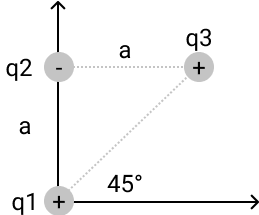
\includegraphics[width=0.3\textwidth]{fe1.png}}
		\caption{Cargas en el espacio}
		\label{fe1}
	\end{figure}
\end{example}

\textit{ Sol. }

\begin{align*}
	F_{23}  & = 9\times 10^9\frac{2\times10^{-6}\cdot 5\times10^{-6}}{(0.1)^2 } = 9N, & F_{13}  & = 9\times 10^9\frac{5\times10^{-6}\cdot 5\times10^{-6}}{(0{.}14)^2 } = 11{.}47N \\
	Fx_{13} & = 11{.}7(\cos(45^{\circ}))= 8{.}11N                                     & Fy_{13} & = 11{.}47N(Sin(45^{\circ}))= 8.11N                                              \\
	F_{x}   & = 8{.}11N -9N = -0{.}89N                                                & F_{y}   & = 8{.}11 +0 = 8{.}11N                                                           \\
	F_{r}   & = 8{.}.11i - 0{.}89j
\end{align*}

\begin{example}
	Tres cargas puntuales se encuentran sobre el eje $x$, la carga positiva $q_{1}=15\mu C$ y está a
	$x=2m$, la carga positiva $1_{2}=6\mu C$ y está en el origen; La fuerza neta que actúa sobre $q_{3}$
	es $0$, ¿Cuál es la coordenada $x$ de $q_{3}$ en la figura\ref{fe2}?
	\begin{figure}[h!]
		\centerline{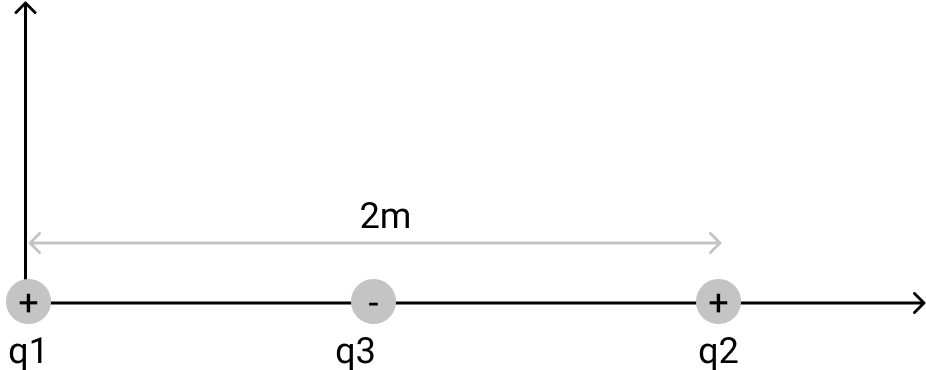
\includegraphics[width=0.7\textwidth]{fe2.png}}
		\caption{Cargas en el eje $x$}
		\label{fe2}
	\end{figure}
\end{example}

\textit{ Sol. }

\begin{align*}
	F_{23}= k \frac{q_{1}q_{2}}{(2)^2 },  F_{31} & = k \frac{q_{1}q_{2}}{(2-x)^2 } & 0     & = 9\mu C x^2  + 24\mu C x -24\mu C                                            \\
	F_{r}=0=F_{23}                               & =F_{31}                         & x     & = \frac{-24\pm \sqrt{(24)^2 -4(9)(24)} }{2(9)}= \frac{-24\pm \sqrt{1440}}{18} \\
	k \frac{q_{1}q_{2}}{(2)^2 }                  & =k \frac{q_{1}q_{2}}{(2-x)^2 }  & x_1& = \frac{-24+37{.}95}{18}=0{.}7748m                                            \\
	\frac{q_{2}}{x^2 }                           & =\frac{q_{1}}{(2-x)^2}          & x_{2} & = \frac{-24-37{.}95}{18}=-3{.}44m                                             \\
	(6 \mu C)(4-4x+x{2})                         & =(15\mu C)(x^2 )                &       & Coordenada (x,y)= (0{.}7748 , 0)
\end{align*}

\begin{example}
	Dos esferas idénticas cargadas cada una en una masa de $3 \times 10^{-2}Kg$
	cuelgan en equilibrio. La longitud L de las cuerdas es de $0.15m$
	y el ángulo es de $\theta =5$ Encuentre la magnitud de la carga en cada esfera.
	\begin{figure}[h!]
		\centerline{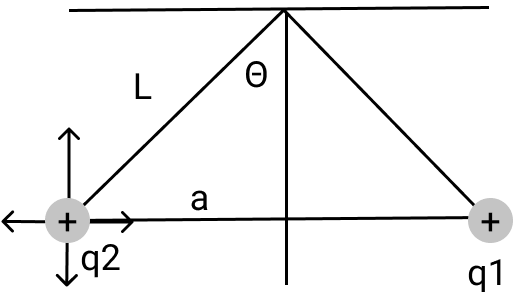
\includegraphics[width=0.6\textwidth]{fe3.png}}
		\caption{Encontrar la magnitud de las cargas}
		\label{fe3}
	\end{figure}
\end{example}

\textit{ Sol. }

Dibujando un diagrama de cuerpo libre en cualquiera de las cargas, debemos tener en cuenta cómo calcular las fuerzas en $T_{x}, T_{y}, P, F_{r}$ y $T$,
donde $T_{x}$ y $T_{y}$ es la tensión en el eje $x$ y $y$ respectivamente, $P$ es el peso ($P=mg$), representado en el eje negativo de las ordenadas, $F_{r}$ es la resistencia del eje $x$
y finalmente $T$ es la fuerza eléctrica en la cuerda. La carga al estar en equilibrio, podemos plantear lo siguiente:

El peso será igual a $p=(3 \times 10^-{2} Kg)(9.81 m/s^2)=0.294N$ y además:
\begin{align*}
	T_{x}-F_{r} & =0 \\
	T_{y}-P     & =0
\end{align*}

Haciendo uso de la trigonometría, si el ángulo interno mide 5$^{\circ}$ quiere decir que sus otros dos ángulos son 90$^{\circ}$ y 85$^{\circ}$,
entonces dentro del diagrama de cuerpo libre se nos forma un triángulo con esos mismo ángulos. Teniendo los datos de las fuerzas
como los catetos e hipotenusa, se plantea:
\begin{align*}
	T_{x}                    & = T \cos 5^{\circ} & \frac{T}{\sin 85^{\circ}}      & = T_{y}  \\
	(0.295N)\cos(85^{\circ}) & = 0.025N           & \frac{0.294N}{\sin 85^{\circ}} & = 0.295N
\end{align*}


El otro dato que nos falta encontrar es la separación entre las dos cargas, como usaremos solo la mitad de la base del triángulo, decimos que $a=\frac{d}{2}$
usando la propiedad de los triángulos rectángulos: $d=2(0.15m)\sin (5^{\circ})=0.026$; Ahora despejamos la carga de la fórmula \eqref{eqCoulomb}:
\begin{align*}
	T & = k \frac{q^2 }{(d)^2}                       \\
	q & = \frac{\sqrt{(0.025N)(0.026m)^2 }}{9x10^9C} \\
	q & = 4.33x10^{-8}C
\end{align*}

Finalmente, la magnitud de la fuerza de las dos cargas es $4.33x10^{-8}C$


\subsubsection{Corriente eléctrica}

Es la carga total que pasa a través del área de una sección transversal por unidad de tiempo

\begin{figure}[h!]
	\centerline{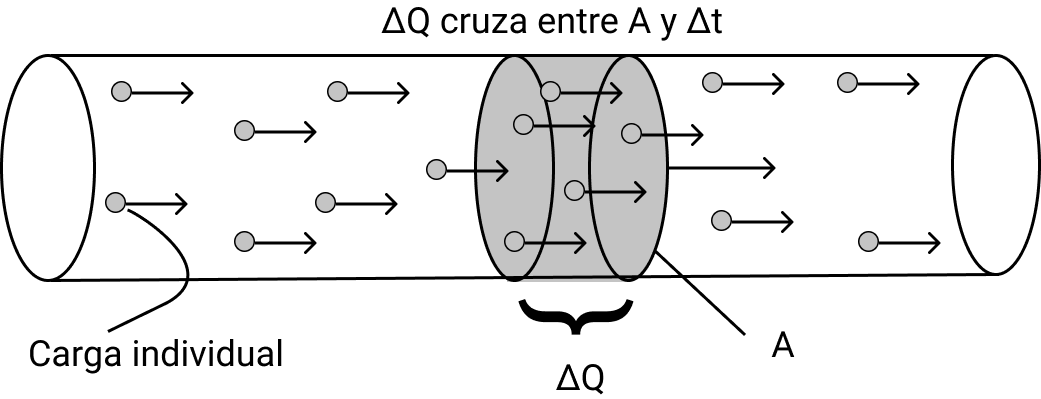
\includegraphics[width=0.7\textwidth]{fe4.png}}
	\caption{Representación gráfica de una corriente eléctrica}
	\label{fe4}
\end{figure}


\begin{equation}
	I= \lim_{\Delta  \to 0} \frac{\Delta Q}{\Delta t} = \frac{dQ}{dt}\left[\frac{C}{s} = A\right]
\end{equation}

Si la corriente no cambia con el tiempo y permanece constante, la llamamos corriente directa
por ejemplo una computadora o celular son de corriente directa.

\begin{figure}[h!]
	\centerline{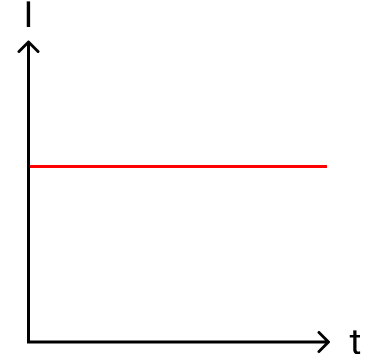
\includegraphics[width=0.2\textwidth]{fe5.png}}
	\caption{Función constante}
	\label{fe5}
\end{figure}

\begin{definition}[Ley de Ohm]
	Establece que la diferencia de potencial $V$ que aplicamos entre los extremos de un conductor determinado es directamente proporcional a la intensidad de la corriente $I$ que circula por el citado conductor. Ohm completó la ley introduciendo la noción de resistencia eléctrica $R$;
\end{definition}

\begin{equation}
	V=R \cdot I
	\label{ohm}
\end{equation}

La corriente alterna es una corriente que varía sinusoidalmente con el tiempo.

\begin{figure}[h!]
	\centerline{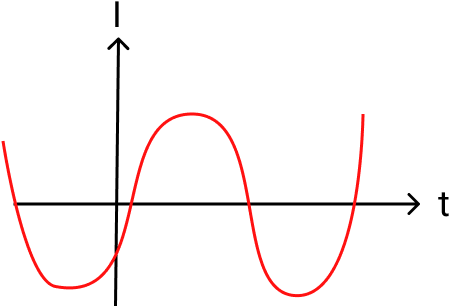
\includegraphics[width=0.4\textwidth]{fe6.png}}
	\caption{Función sinusoidal}
	\label{fe6}
\end{figure}


\begin{definition}[Voltaje]
	Es el trabajo que se debe realizar para mover una carga entre dos puntos de un circuito.
	\begin{equation}
		v_{ab}= \frac{dw}{dq}
	\end{equation}
	donde $w$ es la energía en $j$ (Joules) y $q$ es la carga en $c$ (Coulomb)
\end{definition}

\begin{definition}[Potencia]
	Otra forma de definir el voltaje es con la potencia. La potencia representa cuánta energía por segundo se utiliza para
	alimentar un circuito
\end{definition}

\begin{equation}
	W= \frac{J}{s}
\end{equation}

\begin{equation*}
	P= \frac{dw}{dt} =\frac{dw}{dq} \cdot \frac{dq}{dt} = VI
\end{equation*}

\begin{example} Calcular la potencia en el siguiente circuito:
	\begin{center}
		\begin{circuitikz}[american]
			\centering
			\draw (0,0) to [V=5v] (0,3) to [,R=$220\Omega$] (2,3) ;
			\draw (2,3) to (4,3);
			\draw (4,3) to (6,3) to [D, l=$25mA$](6,0) to (3,0) to (0,0);
		\end{circuitikz}
	\end{center}

	\begin{align*}
		 & P=VI &  & (5v)(25mA)=125Wh
	\end{align*}

\end{example}

\begin{definition}[Potencia disipada]
	Es cuánta potencia disipa por calor por la potencia, se refiere más a calor
	\begin{align*}
		 & P=I \times V &  & P=I^2  \times R &  & P=\frac{V^2 }{R}
	\end{align*}
\end{definition}

\begin{definition}[Resistencia]
	Los materiales en general tienen un comportamiento de resistirse al flujo de carga eléctrica.
	Esta propiedad física, o capacidad para resistirse a la corriente, es conocido como resistencia
	y está representado por la letra $\Omega$.
	\begin{center}
		\begin{circuitikz}[american]
			\draw (0,0)  to [short,  o-o, R=$+v-$] (3,0);
		\end{circuitikz}
	\end{center}
\end{definition}

\begin{figure}[h!]
	\centerline{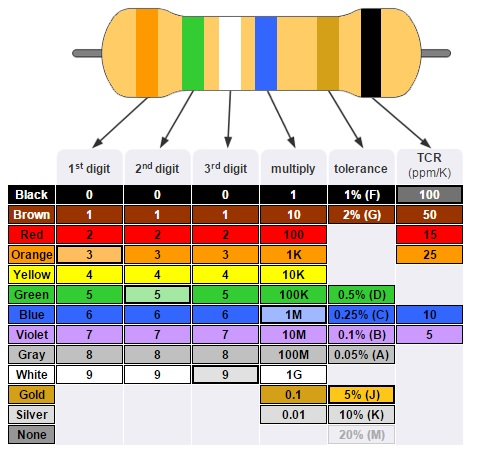
\includegraphics[width=0.7\textwidth]{fe7.jpg}}
	\caption{tabla de códigos de colores estándar EIA}
	\label{fe7}
\end{figure}

\subsubsection{Simbología}
\begin{circuitikz}[american]
	\draw (0,0) to [R=R] (3,0);
	\draw (5,0) to [european resistor] (8,0);
\end{circuitikz}

Existen diferentes tipos de resistencia:
\begin{itemize}
	\item Común
	\item Alta potencia
	\item LDR
	\item variable
	\item Potenciómetro
	\item Termistor
\end{itemize}


\section{Circuitos en serie y paralelo}

En un circuito en serie, la corriente es la misma y fluye por donde haya menos resistencia.

\begin{center}
	\begin{tikzpicture}[american]
		\draw (0,0) to [battery1] (0,3) to (2,3);
		\draw (2,3) to [R=$R_{1}$](4,3);
		\draw (4,3) to (6,3) to [R=$R_{2}$](6,0) to [R=$R_{3}$](0,0);
		\draw [->,>= stealth](7, 1.5) to (9,1.5);
		\draw (10,0) to [battery1] (10,3) to  (13,3);
		\draw (13,3)to [R=$R_{eq}$](13,0) to(10,0);
	\end{tikzpicture}
\end{center}

\begin{center}
	\begin{tikzpicture}[american]
		\draw (0,0) to [battery1](0,3) -- (2,3) to[R=$R_1$] (2,0) -- (0,0);
		\draw (2,3) -- (4,3) to[R=$R_2$](4,0) -- (2,0);
		\draw (4,3) to (6,3) to [R=$R_3$](6,0) to (4,0);
		\draw [->, >= stealth](7, 1.5) to (9, 1.5);
		\draw (10,0) to [battery1] (10,3) to (13,3);
		\draw (13,3) to [R=$R_{eq}$](13,0) to (10,0);
	\end{tikzpicture}
\end{center}

\begin{center}
	\begin{tikzpicture}[american]
		\draw (0,0) to [battery1](0,3) to [R=$R_2$](2,3);
		\draw (2,3) -- (4,3) to [R=$R_2$](4,0);
		\draw (4,3) to (6,3) to [R=$R_3$](6,0) to (0,0);
		\draw [->, >= stealth](7, 1.5) to (9, 1.5);
		\draw (10,0) to [battery1] (10,3) to (13,3);
		\draw (13,3)to [R=$R_{eq}$](13,0) to (10,0);
	\end{tikzpicture}
\end{center}

\subsection{Circuito en serie}

La tensión total de los elementos conectados en serie es la suma de cada una de las tensiones en cada elemento:
\begin{equation}
	V=V_{1}+V_{2}+V_{3}
\end{equation}
La ley de Ohm funciona de la siguiente manera:
\begin{equation}
	V= R_{1}I+ R_{2}I+R_{3}I = (R_{1}+ R_{2}+ R_{3})I = RI
\end{equation}
La resistencia total de todos los receptores conectados en serie en la suma de la resistencia de cada receptor.
\begin{equation}
	R=R_{1}+ R_{2}+ R_{3}
\end{equation}
La corriente es la misma en todo el circuito
\begin{equation}
	I=I_1= I_{2} = I_{3}
\end{equation}

\begin{example}
	la corriente en la figura es de $0.125 A$ en la dirección mostrada.
	Para cada uno de los siguientes pares de puntos ¿Cuál es la diferencia de potencial y cuál punto está al mayor potencial?
	Siendo $A$ donde inicia el circuito y $E$ el final. 1) $\overline{AB}$; 2) $\overline{BC}$; 3) $\overline{CD}$; 4) $\overline{DE}$; 5) $\overline{CE}$; 6)$\overline{EC}$
\end{example}

\begin{center}
	\begin{circuitikz}[american]
		\draw (0,0) to [R=$3\Omega$] (0,3) to [,R=$10\Omega$] (2,3) ;
		\draw (2,3) to (4,3);
		\draw (4,3) to [V=$9V$](6,3) to [R=$5 \Omega $](6,0) to [R=$6\Omega$](3,0) to [V=$12V$,i=$0.125A$](0,0);
	\end{circuitikz}
\end{center}

\begin{enumerate}
	\item $V_{AB} = IR= (0.125A)(10\Omega)=-1.25v$
	\item $V_{BC}=-9v$ Es caída de potencial (potencial negativo) pues va de más a menos.
	\item $V_{CD}$: $(-0.125A)(5\Omega +6\Omega)=(0.125A)(11\Omega)=-1.38v$
	\item $V_{DE}=12v$, su signo es positivo pues su dirección es de menos a más.
	\item $V_{CE}=-1.375v+12v= 10.625v$
	\item $V_{EC}= (-0.125A)(3\Omega)-(0.125A)(10 \Omega)-9V=-10.625v$.
\end{enumerate}

\subsection{Divisor de voltaje}

\begin{center}
	\begin{tikzpicture}[american]
		\draw (1,0) to [open, v=$v_{in}$] (1,3) -- (2,3);
		\draw [short, -*](2,3) to [short, -*] (4,3) to[R=$R_1$](4,1.5) to [ R=$R_2$](4,0);
		\draw (4,3) -- (6,3) to [open, v=$v_{1}$](6,1.5) to [open, v=$v_{out}$](6,0) -- (1,0);
		\draw (6,1.5) -- (4,1.5);
	\end{tikzpicture}
\end{center}

\begin{align*}
	V_1& =V_{in} \frac{R_{1}}{R_{1}+R_{2}} & V_{2} & =V_{out} \frac{R_{2}}{R_{1}+R_{2}} \\
\end{align*}

\subsection{Divisor de corriente}

\begin{center}
	\begin{tikzpicture}[american]
		\draw (0,0) to[open] (0,3) to [I=$I_{in}$](4,3);
		\draw (2,3) to [short, -*](4,3) to[R=$R_1$,-*,i=$I_{1}$] (4,0);
		\draw(4,3) to (6,3) to[R=$R_2$, i=$I_{2}$] (6,0) to (0,0);
	\end{tikzpicture}
\end{center}

\begin{equation}
	I_{1}= \frac{R_{2}}{R_{1}+R_{2}} \cdot I
\end{equation}

\begin{example}
	Una corriente de $3A$ fluye a través de un alambre, como se muestra ¿Cuál será la lectura en un voltímetro cuando se conecta de $AB$, de $AC$ y de $AD$?

	\begin{circuitikz}[american]
		\draw (0,0) to [,R=$6 \Omega$,i=$3A$] (3,0);
		\draw (3,0) to [V=8V](6,0);
		\draw(6,0) to [R=$3\Omega$] (9,0);
		\draw (9,0) to [V=7V](12,0);
	\end{circuitikz}

	\textit{ Sol. }

	\begin{enumerate}
		\item $V_{AB}= -3(6)= -18$
		\item $V_{AC}=-18v-8v-(3A)(3\Omega)=-35v$
		\item $V_{AD}=-18v-8v-9v+7v=-28v$
	\end{enumerate}
\end{example}

\begin{example}
	Una batería con resistencia de $1\Omega$ se conecta en serie con dos resistores. Calcule la corriente del circuito

	\begin{center}
		\begin{tikzpicture}[american]
			\draw (0,0) to (0,3) to  [V=18V](2,3) ;
			\draw (2,3) to (4,3);
			\draw (6,0) to [I=$I$](6,3);
			\draw (4,3) to [R=$1\Omega$](6,3) to (6,0) to [R=$5\Omega$](3,0) to [R= $12\Omega$](0,0);
		\end{tikzpicture}
	\end{center}

\end{example}

\textit{ Sol. }

\begin{equation*}
	R_{eq}= 5\Omega + 12\Omega+1\Omega=18\Omega
\end{equation*}
Al aplicar la ley \ref{ohm} (ley de ohm), se tiene
$I= \frac{V}{R}= \frac{18V}{18\Omega}= 1A$

\subsection{Circuitos en paralelo}
La tensión total es a la suma de todas las fuentes conectadas en paralelo:
\begin{equation}
	I=I_{1}+I_{2}+ \ldots +I_{n}
\end{equation}
\begin{equation}
	I= \frac{V}{R_{1}}+\frac{V}{R_{2}}+ \ldots +\frac{V}{R_{n}}= \left(\frac{1}{R_{1}}+\frac{1}{R_{2}}+ \ldots +\frac{1}{R_{n}}\right)V =\frac{V}{R}
\end{equation}
La resistencia total es la suma de la inversa todas las resistencias.
\begin{equation}
	\frac{1}{R}=\frac{1}{R_{1}}+\frac{1}{R_{2}}+ \ldots +\frac{1}{R_{N}}
\end{equation}
La fuerza generada por el voltaje, llega por igual a todos los elementos.
\begin{equation}
	V= V_{1}=V_{2}=V_{n}
\end{equation}

\begin{example}
	Determine las lecturas del amperímetro y del voltímetro en el circuito

	\begin{center}
		\begin{circuitikz}[american]
			\draw (0,0) to [ammeter] (0,3);
			\draw (0,3) to [V=$6V$] (2,3);
			\draw (5,3) to [voltmeter](3,0);
			\draw (2,3) to [R=$3\Omega$](4,3) to (6,3);
			\draw (9,3) to [V=$6V$](6,3);
			\draw (9,3) to [V=$8V$, i=$I$](9,0);
			\draw (9,0) to [R=$9\Omega$](6,0) to (3,0);
			\draw (3,0) to [R=$4\Omega$](0,0);
		\end{circuitikz}
	\end{center}
\end{example}

\textit{ Sol. }

Para el amperímetro, usamos la fórmula \ref{ohm} que dice $I=\frac{V}{R}$, reemplazamos los datos
$I=\frac{8v+6v-6v}{9\Omega+4\Omega+3\Omega} = \frac{8V}{16\Omega}=0.5A$.
En el voltímetro ideal, es decir en un circuito abierto, el amperímetro ideal (que tenga el mismo potencial eléctrico),
se encuentra la diferencia entre $\left\lvert \sqrt{A}B \right\rvert$,
es decir $-6v+8V-(9\times 0.5)=-2.5V$. Así que el voltímetro marca $2.5v$

\begin{example}[Corriente, resistencia y ley de Ohm]
	Se sabe que la diferencia de potencial a través de la resistencia de $6\Omega$ en la figura,
	es de $48V$ Determine la corriente $I$ que entra, la diferencia de potencial en la resistencia de
	$8\Omega$, la diferencia de potencial a través de la resistencia de $10\Omega$ y la diferencia de
	potencial de $a$ a $b$.
	\begin{center}
		\begin{circuitikz}[american]
			\draw (0,0) to [R=$8\Omega$](3,0);
			\draw (3,0) to (3,1);
			\draw (1,1) to (5,1);
			\draw (1,3) to (5,3);
			\draw (3,3) to [R=$15\Omega$](3,1);
			\draw (1,1) to [R=$30\Omega$](1,3);
			\draw (1,3) to [R= $12\Omega$](1,5);
			\draw (1,5) to (5,5);
			\draw (5,5) to [R=$6\Omega$, I=$48V$](5,3);
			\draw (5,5) to (5,3);
			\draw (5,3) to [R=$10\Omega$](5,1);
			\draw (3,5) to (3,6);
			\draw (0,6) to [I=$I$](3,6);
		\end{circuitikz}
	\end{center}
\end{example}


\textit{ Sol. }

Para encontrar cuánta corriente pasa, aplicamos ley de Ohm:
$V=RI$, despejando nos dá $I_{1}= \frac{48\Omega}{6v}=8A$ e
$I_{2}= \frac{48\Omega}{12v}=4A$. La suma total de la corriente es $I=8A+4A=12A$,
La resistencia equivalente del circuito en paralelo será $R_{e1}= \frac{1}{6}+ \frac{1}{12}=4\Omega$ y $R_{e2}= \frac{1}{30}+\frac{1}{15}+\frac{1}{10}=5\Omega$.
Finalmente se suman las resistencias equivalentes: $R_{e}=8\Omega+5\Omega+4\Omega=17\Omega$ y además el voltaje total es $V=(17\Omega)(12A)=204v$

Ahora se calcula la diferencia de potencial. al sumar los voltajes debería dar igual a 204$v$.
\begin{itemize}
	\item $V_{1}=(4\Omega)(12A)=48v$
	\item $V_{2}=(8\Omega)(12A)=96v$
	\item $V_{3}=(5\Omega)(12A)=60v$
\end{itemize}
Se comprueba que 48$v$+96$v$+60$v$=204$v$

\subsection{Análisis de circuitos de corriente directa}

\begin{align*}
	 & \textbf{Corriente eléctrica} &  & \textbf{Capacitancia}               &  & \textbf{Inductancia} \\
	 & V=RI                         &  & Q=CV,\frac{dq}{dt}=C, \frac{dv}{dt} &  & v=l\frac{di}{dt}     \\
	 & \begin{circuitikz}[american]
		   \draw (0,0) to [R] (3,0);
	   \end{circuitikz} &  & \begin{circuitikz}[american]
		                         \draw (0,0) to [capacitor] (3,0);
	                         \end{circuitikz}   &  & \begin{circuitikz}[american]
		                                                 \draw (0,0) to [L](3,0);
	                                                 \end{circuitikz}
\end{align*}

\subsubsection{Redes en serie}

Sólo cuentan con una terminal en común, es decir una terminal de un elemento se encuentra conectada solamente a una terminal del otro elemento.
El punto común entre los dos elementos no se encuentra conectado en otro elemento que transporta corriente.

\begin{center}
	\begin{tikzpicture}[american]
		\draw (0,0) to [battery1,  *-*] (0,3) to (2,3) ;
		\draw (2,3) to [,R=$R_{1}$](4,3);
		\draw (4,3) to (6,3) to [R=$R_{2}$,  *-*](6,0) to (0,0);
	\end{tikzpicture}
\end{center}


\begin{equation}
	R_{T}= \frac{R_{1}R_{2}}{R_{1}+R_{2}}
\end{equation}


\begin{definition}[Nodo]
	Es un elemento del circuito que une dos o más ramas: $\cdot$
\end{definition}

\begin{definition}[Rama]
	Es un elemento del circuito que contiene una resistencia, un capacitor, una batería, etc.
	\begin{circuitikz}
		\draw (0,0) to[R, *-*] (2,0);
	\end{circuitikz}
\end{definition}

\begin{definition}[Malla]
	Es una trayectoria cerrada en un circuito compuesto por nodos y ramas.

	\begin{center}
		\begin{tikzpicture}[american]
			\draw (0,0) to [R=$R_{1}$,*-*](0,3) to (4,3);
			\draw (2,3) to [R=$R_2$, *-*](2,0);
			\draw (4,3) to[R=$R_3$,*-*] (4,0);
			\draw(4,3) to (6,3) to [R=$R_4$,*-*](6,0) to (0,0);
		\end{tikzpicture}
	\end{center}
\end{definition}

\section{Leyes de Kirchhoff}

\begin{definition}[Primera ley de Kirchhoff, Regla de los nodos]
	La suma de las corrientes que entran a un nodo es igual a la suma de las corrientes que salen de él.

	\begin{equation}
		\sum I_{in}= \sum I_{out}
	\end{equation}
\end{definition}

\begin{definition}[Segunda ley de Kirchhoff, Regla de las mallas]
	La suma de elevaciones y caídas de voltaje dentro de una malla es igual a cero

	\begin{equation}
		\sum v=0
	\end{equation}
\end{definition}

\begin{definition}[Ley de los voltajes de Kirchhoff]
	\begin{equation}
		\sum \Delta V=0
	\end{equation}
\end{definition}

\begin{center}
	\begin{circuitikz}
		\draw (0,0) to [V=$5V$] (0,3) to [R=$R_{1}$] (2,3) ;
		\draw (2,3) to (4,3);
		\draw (4,3) to [V=$4V$](6,3) to [R=$R_{2}$](6,0) to [V=$3V$](3,0) to [R=$R_{3}$](0,0);
	\end{circuitikz}
\end{center}

La caída de potencial es $5V-IR_{1}+4V-IR_{2}-3V-IR_{3}=0$

\begin{center}
	\begin{circuitikz}[
			bigR/.style={R, bipoles/length=3cm}
		]
		\draw (0,2) to [R=$R$, *-*] ++ (4,0)[label=B];
	\end{circuitikz}
\end{center}

\begin{center}
	\begin{equation}
		\Delta V_{ab}=-IR
	\end{equation}
\end{center}

\begin{center}
	\begin{circuitikz}
		\draw (0,0) to [battery=$3V$, *-*](4,0);
	\end{circuitikz}
\end{center}

\begin{center}
	\begin{equation*}
		\Delta V_{ab}=V_{b}-V_{a}=+3V
	\end{equation*}
\end{center}

véase a continuación un circuito como ejemplo:

\begin{center}
	\begin{circuitikz}
		\draw (0,0) to[R=$R_2{=}8k\Omega$] (0,3) to [R=$R_1{=}4k\Omega$](2,3) to[R=$R_4{=}24k\Omega$] (2,0) to [R=$R_3{=}12k\Omega$] (0,0);
		\draw (2,3) to (5,3);
		\draw (5.5,0) to [R=$R_5{=}12k\Omega$](1.5,0);
		\draw (5.5,0) to [battery1=$72V$](5.5,3);
		\draw(5,3) to [R=$R_6{=}12k\Omega$](9,3) to[R=$R_7{=}9k\Omega$] (7,0) to (5.5,0);
		\draw (9,3) to [R=$R_8{=}3k\Omega$](12,0);
		\draw (12,0) to [R=$R_9{=}6k\Omega$](7,0);
	\end{circuitikz}
\end{center}

\begin{align*}
&I_{5}=\frac{E}{R_{1,2,3,4}+R_{5}}=\frac{72V}{24k\Omega}=3mA\\
&V_{7}=\frac{R_{7,8,9}\cdot E}{R_{7,8,9}+R_{6}}=\frac{4.5k\Omega \cdot 72V}{4.5k\Omega+12k\Omega}=\frac{324V}{16.5}=19.6V\\
&I_{7}=\frac{V_{7}}{R_{7,8,9}}=\frac{19.6V}{4.5k\Omega}=4.35mA\\
&I_{6}= \frac{72V}{16.5k\Omega}=4.3mA \\
&I_{4}=I_{5}+I_{6}=3mA+4.3mA = 7.3mA
\end{align*}

%%%%%%%%%%%%%%%%%%%%% PENDIENTE URGENTE

Ahora véase un clásico, encontrar las correntes del siguiente circuito:

\begin{center}
	\begin{circuitikz}
		\draw (0,0) to [battery=$V_{0}$](0,6);
		\draw (0,6) to [R=$R_{1}$, I=$I_{1}$](5,6);
		\draw (0,0) to (5,0);
		\draw (5,6) to (5,5);
		\draw (5,5) to [R=$R_{2}$, I=$I_{2}$](3,3);
		\draw (5,5) to [R=$R_{3}$, I=$I_{3}$](7,3);
		\draw (3,3) to [R=$R_{5}$, I=$I_{5}$](5,1);
		\draw (7,3) to [R=$R_{6}$, I=$I_{6}$](5,1);
		\draw (3,3) to [R=$R_{4}$, I=$I_{4}$](7,3);
		\draw (5,0) to (5,1);
	\end{circuitikz}
\end{center}

Las ecuaciones resultantes son obtenidas de las leyes de la corriente de Kirchhoff:

\begin{align*}
	 & I_{1}=I_{2}+I_{3} \\
	 & I_{2}=I_{5}+I_{4} \\
	 & I_{6}=I_{3}+I_{4}
\end{align*}
Las ecuaciones resultantes son resultado de aplicar las leyes del voltaje de Kirchhoff
\begin{align*}
	 & V_{0}-I_{1}R_{2}-I_{1}R_{2}-I_{5}R_{5}=0 \\
	 & -I_{3}R_{3}+I_{4}R_{4}+I_{3}R_{3}=0      \\
	 & -I_{6}R_{6}+I_{5}R_{5}-I_{3}R_{3}=0
\end{align*}

Usando este circuito podemos hacer un ejemplo teniendo las resistencias $R_{1}=1,R_{2}=2\ldots R_{6}=6$ y el voltaje inicial $V_{0}=10V$,
encontrar $I_{1}$ a $I_{6}$ y $V_{1}$ a $V_{6}$.

\begin{example}
	Encuentre las corrientes si el interruptor está abierto y cuando está cerrado:
	\begin{center}
		\begin{tikzpicture}[american]
			\draw (0,0) to [I=$I_{1}$](0,3);
			\draw (2,3) to [battery1=$12v$](0,3);
			\draw (2,3) to (4,3);
			\draw (3,3) to (3,2.5);
			\draw (3,0) to [R=$4\Omega $, I=$I_{3}$](3,1.5);
			\draw (3,1.5) to (3.5,2.5);
			\draw (6,3) to [I=$I_{2}$](6,0);
			\draw (4,3) to [battery1=$9V$](6,3) to (6,0) to [R=$8\Omega$](3,0) to [R= $7\Omega$](0,0);
		\end{tikzpicture}

	\end{center}
\end{example}

\textit{ Sol. }

Se debe resolver un sistema de ecuaciones con las ecuaciones obtenidas:

\begin{align*}
	 & -I_{1}+I_{2}-I_{3}    & =0    \\
	 & 0I_{1}-8I_{2}-4I_{3}  & =9V   \\
	 & -7I_{1}+0I_{2}+4I_{3} & =-12V
\end{align*}
\begin{align*}
	\Delta       & = \begin{bmatrix}
		                 -1 & 1  & -1 \\
		                 0  & -8 & -4 \\
		                 -7 & 0  & 4
	                 \end{bmatrix}=116 & \Delta x_1& = \begin{bmatrix}
		                                                      0  & 1  & -1 \\
		                                                      8  & -8 & -4 \\
		                                                      12 & 0  & 4
	                                                      \end{bmatrix}=108  \\
	\Delta x_{2} & = \begin{bmatrix}
		                 -1 & 0   & -1 \\
		                 0  & 9   & -4 \\
		                 7  & -12 & 4
	                 \end{bmatrix}=-51 & \Delta x_{3} & = \begin{bmatrix}
		                                                      -1 & 1  & 0   \\
		                                                      0  & -8 & 9   \\
		                                                      7  & 0  & -12
	                                                      \end{bmatrix}=-159
\end{align*}

Una $v$, es calculada de las matrices, para encontrar las tres variables de la corriente y evitar hacer el método de eliminación,
se usó un método sencillo llamado determinantes:

\begin{align*}
	 & I_{1}=\frac{\Delta x_{1}}{\Delta}=\frac{108}{116}=0.93A   &
	 & I_{2}=\frac{\Delta x_{2}}{\Delta}=\frac{-51}{116}=-0.43A  &
	 & I_{3}=\frac{\Delta x_{3}}{\Delta}=\frac{-159}{116}=-1.37A
\end{align*}

\begin{example}
	Usando la ley de Kirchhoff, podemos resolver el siguiente circuito:
	\begin{center}
		\begin{tikzpicture}
			\draw (0,0) to [V=$V_{s}$] (0,6) to  [I=$i$](2,6);
			\draw (2,6) to [R=$R$](2,3) to [cute inductor=$L$,*-*](2,0) to(0,0); \hspace{3cm} $V_{s}-iR-L \frac{di}{d}=0$
		\end{tikzpicture}
	\end{center}

	Si $V_{s}=V=\text{Constante}$, entonces:
	\begin{align*}
		\frac{di}{dt}+\frac{R}{L}u=\frac{V}{L} &  & \int e^{\frac{R}{L}} dt= \frac{V}{R} \left( 1-e^{-R/L} \right) \\
	\end{align*}
\end{example}

\begin{center}
	\textbf{Fuentes de voltajes DC}

	\begin{circuitikz}

		\draw (0,0) to [american voltage source, label=ideal $Vs$] (2,0) ;
		\draw (2.5,0) to [battery, label=batería](4.5,0);
	\end{circuitikz}
\end{center}

\begin{center}
	\textbf{Fuentes de corriente DC}

	\begin{circuitikz}
		\draw (0,0) to [american current source, label=ideal $Is$] (2,0) ;
	\end{circuitikz}
\end{center}


La transformación de fuentes es el proceso de reemplazar una fuente de voltaje en serie $V_{s}$ con un resistor $R$ por una corriente $I_{s}$ en paralelo con una resistencia $R$ o viceversa

\begin{center}
	\begin{circuitikz}
		\draw (0,0) to [V=$V_{s}$] (0,3) to [R=$R$] (2,3) ;
		\draw (2,3) to (3,3);
		\draw (3,0) to (0,0);
		\draw [<->,>=stealth] (4,1.5) -- (5,1.5);
		\draw (7,0) to [I=$i_{s}$] (7,3) to (9,3) ;
		\draw(9,3) to [R=$R$](9,0);
		\draw (9,3) to (10,3);
		\draw (10,0) to (7,0);
	\end{circuitikz}
\end{center}

\begin{equation}
	v_{s}=i_{s}R
\end{equation}

\begin{definition}[Fuentes de corriente en paralelo]
	Si dos o más fuentes de corriente están en paralelo, todas pueden ser reemplazadas por una fuente de corriente que tenga la magnitud y dirección de la resultante.
\end{definition}
\
\begin{definition}[Fuentes de voltaje en paralelo]
	Si dos o más fuentes de voltaje están en paralelo, todas pueden ser reemplazadas por una fuente de voltaje resultante.
\end{definition}

\begin{example}
	Usa la transformación de fuentes para encontrar $v_{0}$, donde está la resistencia de $8\Omega$:
	\begin{center}
		\begin{tikzpicture}[american]
			\draw (0,0) to [R=$4\Omega$](0,3);
			\draw (2,3) to [I=$3A$](2,0);
			\draw (0,3) to (2,3);
			\draw (2,3) to [R=$2\Omega$](4,3) to[R=$8\Omega$] (4,0);
			\draw(4,3) to [R=$3\Omega$](6,3) to [V=$12V$](6,0) to (0,0);
		\end{tikzpicture}
	\end{center}

	Primero se transforman las fuentes de voltaje, se combina el resistor $4$ y $6\Omega$
	y transformando la fuente de 12V obtenemos:
	\begin{center}
		\begin{tikzpicture}[american]
			\draw (0,0) to [V=$12V$](0,3);
			\draw (0,3) to [R=$4\Omega$](2,3);
			\draw (2,3) to [R=$2\Omega$](4,3) to [R=$8\Omega$] (4,0);
			\draw(4,3) to (6,3) to [R=$3\Omega$](6,0) to (0,0);
			\draw (6,3) to (9,3) to [I=$4A$](9,0) to (6,0);
		\end{tikzpicture}
	\end{center}
	\vspace{1cm}
	\begin{center}
		\begin{tikzpicture}[american]
			\draw (4,3) to (0,3) to [I=$2A$](0,0);
			\draw (2,3) to [R=$6\Omega$](2,0);
			\draw (0,3) to (2,3);
			\draw (2,3) to (4,3) to [R=$8\Omega$] (4,0);
			\draw(4,3) to(6,3) to [R=$3\Omega$](6,0) to (0,0);
			\draw (6,3) to (9,3);
			\draw (6,0) to (9,0) to [I=$4A$](9,3);
		\end{tikzpicture}
	\end{center}

	Ahora obtenemos las resistencias de 3 y 6 Ohms en paralelo, también combinamos las fuentes de corriente de $2A$ y $4A$.
	\begin{center}
		\begin{tikzpicture}[american]
			\draw (4,3) to (0,3) to [R=$8\Omega$, I=$i$](0,0);
			\draw (2,3) to [R=$2\Omega$](2,0);
			\draw (0,3) to (2,3);
			\draw (2,3) to (4,3);
			\draw (0,0) to (4,0) to [I=$2A$](4,3);
		\end{tikzpicture}
	\end{center}
	Y utilizando divisor de corriente:
	\begin{center}
		\begin{align*}
			 & i=\frac{2V}{2\Omega +8\Omega}\cdot 2=0.4A \\
			 & v_{0}=8i=9(0.4)=3.2V
		\end{align*}
	\end{center}
\end{example}

\section{Teorema de Thevenin}

\begin{theorem}[Thevenin]
	Cualquier red de corriente directa lineal bilateral de dos terminales puede ser reemplazada por un circuito equivalente que consiste de una fuente de voltaje y un resistor en serie
	\begin{center}
		\begin{circuitikz}
			\draw (0,0) to [battery1=$E_{Th}$] (0,3) to [R=$R_{Th}$] (2,3) ;
			\draw (2,3) to (3,3);
			\draw (3,0) to (0,0);
			\draw [<->,>=stealth] (4,1.5) -- (5,1.5);
			\draw (7,0) to [R=$R_{Th1}$] (7,3) to (9,3);
			\draw (9.5,3) to [battery1=$E_{Th2}$](9,3);
			\draw (9.5,3)to [R=$R_{Th2}$](11,3);
			\draw (11,0) to [battery1=$E_{Th1}$] (7,0);
		\end{circuitikz}
	\end{center}
\end{theorem}

Sustitución del circuito de Thévenin equivalente para una red compleja

\begin{center}
	\begin{tikzpicture}[american]
		\draw (0,0) to[battery1=$E$] (0,3) to
		(2,3) to[R=$R_1$] (2,0) to (0,0);
		\draw (4,0) to [R=$R_3$](4,3);
		\draw (2,3) to [R=$R_2$](4,3);
		\draw (4,0) to (2,0);
		\draw(4,3) to (6,3) to[I=$I_{L}$, vR=$R_L$] (6,0) to (4,0);
		\draw [->,>=stealth] (7,1.5) -- (9,1.5);
		\draw (13,3) to [R=$R_{Th}$](10,3) to [battery1=$E_{Th}$] (10,0);
		\draw (13,3) to [I=$I_{L}$, vR=$R_L$](13,0) to (10,0);
	\end{tikzpicture}
\end{center}

\begin{enumerate}
	\item Retire aquella porción de la red a través de la cual el circuito equivalente de Thévenin va a ser encontrado. En La figura, requiere que el resistor de la carga $RL$ sea temporalmente retirado de la red
	\item Marque las terminales de la restante red de dos terminales.
	\item Calcule $RTh$ estableciendo primero todas las fuentes en cero (Las fuentes por voltaje son reemplazadas por cortocircuitos, y las fuentes de corriente por circuitos abiertos) y encontrando luego la resistencia resultante entre las dos terminales marcadas. (Si la resistencia interna de las fuentes de voltaje y/o corriente es incluida en la red original, debe permanecer cuando las fuentes son puestas en cero).
	\item Calcule $ETg$ devolviendo primero todas las fuentes a sus posiciones originales y encontrando el voltaje de circuito abierto entre las terminales marcadas (Este paso es el que invariablemente conducirá a los mayores errores y confusión. En todos los casos, recuerde que el potencial de circuito abierto entre las dos terminales marcadas en el paso 2).
	\item Trace el circuito equivalente de Thévenin con la porción del circuito previamente retirado reemplazado entre las terminales del circuito equivalente. Este paso está indicado por la colocación del resistor RL entre las terminales del circuito Thévenin equivalente.
\end{enumerate}

\begin{example}
	Encuentre el circuito equivalente de Thévenin para la red ubicada en el área sombreada del circuito y luego encuentre la corriente a través de $R_{L}$ para valores de $2\Omega $, $10\Omega $ y $100\Omega$.
	\begin{tikzpicture}[american]
		\draw (0,3) to[battery1=$9v$, l_=$E_{1}$](0,0);
		\draw (0,3) to [R=$R_1{=}3\Omega$](4,3);
		\draw (3,3) to[R=$R_2{=}6\Omega$](3,0);
		\draw (5.9,3) to [short, l=a](6,3);
		\draw(4,3) to (6,3) to[vR=$R_L$, *-*] (6,0) to (0,0);
		\draw (6,0) to [short, l=b](5.9,0);
	\end{tikzpicture}

	\textit{ Sol. }

	Los pasos 1 y 2 producen el siguiente circuito:

	\begin{equation*}
		E_{th}=\frac{R_{2}E_{1}}{R_{2}+R_{1}}=\frac{(6\Omega)(9V)}{(3\Omega)+(6\Omega)}=\frac{54V}{9}=6V
	\end{equation*}
	\begin{center}
		\begin{tikzpicture}[american]
			\draw (0,3) to [battery1=$E_{1}{=}9V$](0,0);
			\draw (2,3) to [R=$R_{2}{=}6\Omega$](2,0);
			\draw (0,3) to [R=$R_{1}{=}3\Omega$](2,3);
			\draw (2,3) to (4,3);
			\draw (0,0) to (4,0) to [open, *-*](4,3);
		\end{tikzpicture}
	\end{center}

	Reemplazando la fuente de voltaje $E_{I}$ con un corto circuito equivalente se obtiene:

	\begin{equation*}
		R_{th}= R_{1}||R_{2}= \frac{(30\Omega)(6\Omega)}{(30\Omega)+(6\Omega)}=2\Omega
	\end{equation*}
	\begin{center}
		\begin{tikzpicture}[american]
			\draw (2,3) to (0,3) to [battery1=$E_{Th} {=} 6V$] (0,0);
			\draw (2,3) to [R=$R_{Th} {=}2\Omega$](4,3);
			\draw (4,3) to (6,3) to [I=$I_{L}$,vR=$R_{L}$, *-*](6,0) to (0,0);
			\draw (6,0) to [short, l=b](5.9,0);
			\draw (5.9,3) to [short, l=a](6,3);
		\end{tikzpicture}
	\end{center}

	\begin{align*}
		 & I_{L}                  & =\frac{E_{Th}}{R_{Th}+R_{L}}           \\
		 & R_{L}=2\Omega, I_{L}   & =\frac{6V}{2\Omega + 2\Omega}=1.5A     \\
		 & R_{L}=10\Omega, I_{L}  & =\frac{6V}{2\Omega + 10\Omega}=0.5A    \\
		 & R_{L}=100\Omega, I_{L} & =\frac{6V}{2\Omega + 100\Omega}=0.059A
	\end{align*}
\end{example}
\newpage
\section{Teorema de Norton}

\begin{theorem}[Norton]
	Cualquier red de cd lineal bilateral de dos terminales pueden ser reemplazada por un circuito equivalente que consista de una fuente de corriente y un resistor en paralelo:
	\begin{center}
		\begin{circuitikz}
			\draw (0,0) to [I=$I_{N}$] (0,3) to (2,3);
			\draw (2,3) to (3,3);
			\draw (3,3) to [R=$R_{N}$](3,0);
			\draw (0,0) to (3,0);
			\draw (3,0) to [short, -*,label=$a$](5,0);
			\draw (3,3) to [short, -*, label=$b$](5,3);

		\end{circuitikz}
	\end{center}
\end{theorem}

\begin{enumerate}
	\item Retire aquella porción de la red a través de la ual se encuentra el circuito equivalente de Norton
	\item Marque las terminales de la red de dos terminales restantes
	\item Calcule $R_{N}$ estableciendo primero todas las fuentes en cero (las fuentes de voltaje son reemplazadas por cortocircuitos, y las fuentes de corriente por circuitos abiertos) y encontrando entonces la resistencia resultante entre las dos terminales marcadas. (Si la resistencia interna de las fuentes de voltaje y/o corriente se incluye en la red original, debe permanecer cuando las fuentes se establecen en cero). Como $R_{N}=RTh$, el procedimiento y el valor obtenido usando el enfoque descrito por el teorema de Thévenin determinará el valor apropiado de $R_{N}$.
	\item Calcule $I_{N}$ devolviendo primero todas las fuentes a su posición original y encontrando entonces la corriente en cortocircuito entre las terminales marcadas. Es la misma corriente que sería medida por un amperímetro colocado entre las terminales marcadas.
	\item Trace el circuito equivalente de Norton con la posición del circuito previamente retirado, reemplazada entre las terminales del circuito equivalente.
\end{enumerate}

\begin{center}
	\begin{circuitikz}
		\draw (0,0) to [battery1, l=$E_{Th}{=} I_{N}R_{N}$](0,3);
		\draw (0,0) to [battery1](0,3);
		\draw (0,3) to [R, l_=$R_{Th} {=} R_{N}$](3,3);
		\draw (3,0) to (0,0);
		\draw [<->,>=stealth] (4,1.5) -- (5,1.5);
		\draw (7,0) to [I=$I_{N}{=}\frac{E_{Th}}{R_{Th}}$] (7,3) to (9,3) ;
		\draw(9,3) to [R=$R_{N}{=}R_{Th}$](9,0);
		\draw (9,3) to (10,3);
		\draw (10,0) to (7,0);
	\end{circuitikz}
\end{center}

\begin{example}
	Encuentre el circuito equivalente de Norton para la red externa al resistor de $9\Omega$ en la figura:
	\begin{center}
		\begin{tikzpicture}[american]
			\draw (0,0) to [R, l_=$R_{2}{=}4\Omega$] (0,3) to  (2,3) ;
			\draw (2,4) to [R, l_=$R_{1}{=}5\Omega$](4,4);
			\draw (4,4) to (4,2);
			\draw (2,2) to [I, l_=$I{=}10A$](4,2);
			\draw (2,2) to (2,4);
			\draw (4,3) to (5,3) to [short, l=$a$,-*](6,3) to [R=$R_{L}{=}9\Omega$](6,0);
			\draw (0,0) to (5,0) to [short, l=$b$,-*](6,0);
		\end{tikzpicture}
	\end{center}

	\textit{ Sol. }

	Planteamos la Resistencia de nortón:
	\begin{equation*}
		R_{N}=R_{1}+R_{2}=5\Omega + 4\Omega = 9\Omega
	\end{equation*}
	La corriente Norton es la misma que la corriente a través del resistor de $4\Omega$. Aplicando la regla del divisor de corriente:
	\begin{equation*}
		I_{N}=\frac{R_{1}I}{R_{1}+R_{2}}=\frac{(5\Omega)(10A)}{5\Omega + 4\Omega}=5{.}556A
	\end{equation*}
	\begin{center}
		\begin{tikzpicture}[american]
			\draw (0,0) to [R, l_=$R_{2}{=}4\Omega$] (0,3) to  (2,3) ;
			\draw (2,4) to [R, l_=$R_{1}{=}5\Omega$](4,4);
			\draw (4,4) to (4,2);
			\draw (2,2) to [I, l_=$I{=}10A$](4,2);
			\draw (2,2) to (2,4);
			\draw (4,3) to (5,3) to [short, l=$a$,-*](6,3) to [R=$R_{L}{=}9\Omega$](6,0);
			\draw (0,0) to (5,0) to [short, l=$b$,-*](6,0);
			\draw [->,>=stealth] (8,1.5) -- (9,1.5);
			\draw (10,0) to [R, l_=$R_{2}{=}4\Omega$] (10,3) to (12,3) ;
			\draw(12,3) to [I=$10A$](12,0);
			\draw (12,3) to (14,3) to [R, l_=$R_{1}{=}5\Omega$](14,0);
			\draw (14,0) to [short,-*](12,0) to (11,0) to [short, l_=$b$, -*](10,0);
			\draw (10,0) to [short, l=$a$](13,0);
		\end{tikzpicture}
	\end{center}
\end{example}

\subsection{Capacitores}

\textbf{Capacitor}
\begin{center}
	\begin{align*}
		 & Q=CV                         &
		 & \frac{dq}{dt}=C\frac{dv}{dt} &
		\frac{dq}{dt}=i=C\frac{dv}{dt}
	\end{align*}
	\begin{circuitikz}[american]
		\draw (0,0) to [capacitor] (3,0);
	\end{circuitikz}
\end{center}

\textbf{Inductor}
\begin{center}
	\begin{align}
		 & V=L\frac{di}{dt} & \begin{circuitikz}[american]
			                      \draw (0,0) to [cute inductor] (3,0);
		                      \end{circuitikz}
	\end{align}
\end{center}

\begin{definition}[Capacitor]
	Es un elemento pasivo diseñado para almacenar energía en us campo eléctrico. Los condensadires se utilizan ampliamente en la electrónica, las comunicaciones, las computadoras y los sistemas de energía.
	Consiste en dos placas conductoras separadas por un aislante (o dieléctrico).
\end{definition}

Cuando se conecta una fuente de tensión al condensador, la fuente deposita una carga positiva $q$ en un placa y una carga negativa $-q$ en la otra. Se dice que el condensador almacenada, representada por $q$, es directamente proporcional al voltaje aplicado, por lo que
\begin{equation}
	Q=CV
\end{equation}
Donde $Q$ es la constante de proporcionalidad; es la capacitancia en (Faradios [F]), $q$ es la carga en Coulombs.
\begin{equation}
	C=\in \frac{A}{d}
\end{equation}
Donde $\in$ es la permitividad del dieléctrico. El vacío vale 1.0, el aire 1.0006 y el agua destilada 80.

\begin{figure}[h!]
	\centerline{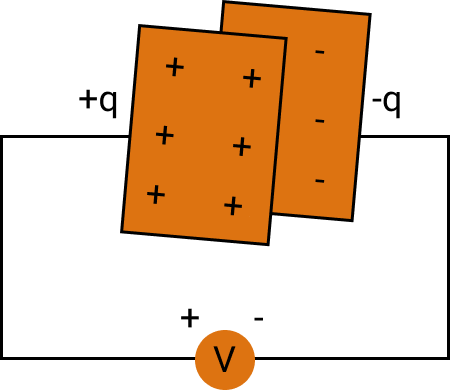
\includegraphics[width=0.25\textwidth]{fe8.png}}
	\caption{Un capacitor en el circuito.}
	\label{fe8}
\end{figure}

Hay dos tipos, los electrolíticos y los variables, consulte la tabla \ref{tabelec2}:
\begin{table}[h!]
	\centering
	\begin{tabular}{|c|c|c|}
		\hline
		Capacitores          & \textbf{Electrolítico}                                                                                                               & \textbf{Variable}                                                                                                      \\ \hline
		Valores típicos      & 0.1 $\mu F$ a 15,000 $\mu F$                                                                                                         & 1.5$pF$ a 600$puF$                                                                                                     \\ \hline
		Intervalo de voltaje & $5V$ a $450V$                                                                                                                        & $5V$ a $100V$                                                                                                          \\ \hline
		Tolerancia           & $\pm 20\%$                                                                                                                           & $\pm 10\%$                                                                                                             \\ \hline
		Aplicaciones         & \begin{tabular}[c]{@{}c@{}}Polarizado, utilizado en\\ fuentes de alimentación de cd,\\ filtros de paso y bloqueo de cd.\end{tabular} & \begin{tabular}[c]{@{}c@{}}No polarizado; utilizado\\ en osciladores, circuitos\\ de sincronización, etc.\end{tabular} \\ \hline
	\end{tabular}
	\caption{Tipos de capacitores}
	\label{tabelec2}
\end{table}


\subsection{Capacitores en paralelo}
\begin{center}
	\begin{tikzpicture}[american]
		\draw (0,0) to[V, l_=$V$] (0,3) --
		(2,3) to[capacitor=$C_{1}$] (2,0) -- (0,0);
		\draw (3,0) to [short, l_=$V_{1}$](3,3);
		\draw (2,3) -- (4,3) to[capacitor=$C_{2}$](4,0) -- (2,0);
		\draw (5,0) to [short, l_=$V_{1}$](5,3);
		\draw(4,3) to (6,3) to[short, l=$V_{2}$] (6,0) to (4,0);
		\draw (6,0) to (8,0) to [capacitor=$C_{3}$](8,3) to (6,3);
	\end{tikzpicture}
\end{center}

\begin{align}
	q      & =q_{1}+q_{2}+q_{3}  \\
	V      & =V_{1}=V_{2}=V_{3}  \\
	C_{eq} & = C_{1}+C_{2}+C_{3}
\end{align}

\subsection{Capacitores en serie}
\begin{center}
	\begin{tikzpicture}[american]
		\draw (0,0) to [V=$V$] (0,3) to  [capacitor=$C_{1}$](2,3) ;
		\draw (0.5,3) to (0.5,1) to  [short, l=$V_{1}$](1.5,1) to (1.5,3);
		\draw (2,3) to [capacitor=$C_{2}$](4,3);
		\draw (2.5,3) to (2.5,1) to  [short, l=$V_{2}$](3.5,1) to (3.5,3);
		\draw (4,3) to [capacitor=$C_{3}$](6,3) to (6,0) to (0,0);
		\draw (4.5,3) to (4.5,1) to  [short, l=$V_{3}$](6,1);
	\end{tikzpicture}
\end{center}

\begin{align}
	 & q                & =q_{1}=q_{2}=q_{3}                                 \\
	 & V                & =V_{1}+V_{2}+V_{3}                                 \\
	 & \frac{1}{C_{eq}} & = \frac{1}{C_{1}}+ \frac{1}{C_{2}}+\frac{1}{C_{3}}
\end{align}

\begin{example}
	Determine la capacitancia equivalente entre los puntos a y b para el grupo de capacitores conectados que se muestran a continuación. Utilice los valores $C_{1}=5\mu F$,
	$C_{2}=10\mu F$  y $C_{3}=2\mu F$
\end{example}

\begin{center}
	\begin{circuitikz}
		\draw (3,3) to [short,  l_=$a$, -*](3,4);
		\draw (0,0) to (0,3) to [capacitor=$C_{1}$] (2,3) ;
		\draw (2,3) to (4,3);
		\draw (4,3) to [capacitor=$C_{1}$](6,3) to (6,0) to [capacitor=$C_{2}$](3,0) to [capacitor=$C_{2}$](0,0);
		\draw (3,3) to (3,-2);
		\draw (3,3) to [capacitor=$C_{3}$](3,0);
		\draw (1,-4) to [capacitor=$C_{2}$](1,-2) to (5,-2) to [capacitor=$C_{2}$](5,-4) to (1,-4);
		\draw (3,-4) to [short,  l_=$b$,-*](3,-5);
	\end{circuitikz}
\end{center}

Se suma en serie $C_{1}$ y $C_{2}$

\begin{align*}
	C_{A}= \frac{5\cdot 10}{5+10} = \frac{10}{3}\mu F &  & C_{B}= \frac{5\cdot 10}{5+10} = \frac{10}{3}\mu F \\
\end{align*}

Se suma a continuación en paralelo $C_{A}$, $C_{B}$ y $C_{3}$, luego se sumará en serie los nuevos $C_{C}$ con $C_{D}$

\begin{align*}
	C_{C} & =\frac{10}{3}\mu F +\frac{10}{3}\mu F+ 2\mu F=8.66 \mu F & C_{D} & =10\mu F+10\mu F=20\mu F \\
\end{align*}

Finalmente se obtiene:

\begin{equation*}
	C=\frac{20\cdot 8.66}{20+ 8.66}= 6.05 \mu F
\end{equation*}

\section{Circuitos RC}

En $t=0$ el interruptor se coloca en la posición 1 y se
considera que el capacitor está descargado.

\begin{center}
	\begin{tikzpicture}[american]
		\draw (0,3) to [battery1=$E$](0,0);
		\draw (2,3) to [short, *-, l_=$1$](0,3);
		\draw (3,3) to [short, *-](4,3);
		\draw (3,3) to (2,4);
		\draw (3,0) to [short, -*, l_=$2$] (3,1.5);
		\draw (6,3) to (6,0);
		\draw (4,3) to [R=$R$, v=$v_R$](6,3) to [curved capacitor=$C$,v=$v_C$ ](6,0) to (3,0) to (0,0);
	\end{tikzpicture}
\end{center}

\begin{align*}
	 & V_{r}+V_{c}=E                                           &  & e^{\int \frac{1}{RC}} dt=e^{\frac{t}{RC}}                                                                                                                                                \\
	 & R\cdot I+V_{C}=E                                        &  & e^{\frac{t}{RC}}\cdot \frac{dv}{dt}+e^{\frac{t}{RC}}\cdot \frac{V_{C}}{RC}=e^{\frac{t}{RC}}\cdot \frac{E}{RC}                                                                            \\
	 & I=i_{R}=I_{C}=C\frac{dv}{dt}                            &  & \frac{d}{dt} \left( Ve^{\frac{t}{RC}} \right )= e^{\frac{t}{RC}}\cdot \frac{e}{RC} \implies \int \frac{d}{dt} \left( Ve^{\frac{t}{RC}} \right )= \int e^{\frac{t}{RC}}\cdot \frac{E}{RC} \\
	 & R\cdot C \frac{dv}{dt}+V_{C}=E                          &  & Ve^{\frac{t}{RC}}= \frac{e^{\frac{t}{RC}}}{\frac{1}{RC}\cdot \frac{E}{RC}} \implies Ve^{\frac{t}{RC}}=E\cdot e^{\frac{t}{RC}}+K                                                          \\
	 & \frac{dv}{dt}+\frac{V_{C}}{R\cdot C}=\frac{E}{R\cdot C} &  & V=E+Ke^{\frac{-t}{RC}}; t=0 \implies V(t)=0 \implies E+k=0                                                                                                                               \\
	 & \frac{dv}{dt}+\frac{V_{C}}{R\cdot C}=\frac{E}{R\cdot C} &  & V=E-Ee^{\frac{-t}{RC}}
\end{align*}

\begin{equation}
	V=E \left( 1-e^{\frac{-t}{RC}} \right )
\end{equation}


la corriente es $i=C \frac{dv}{dt}$

\begin{align*}
	 & \frac{dv}{dt}=\frac{d}{dt} \left( E^{-e^\frac{-t}{RC}} \right)                                                               \\
	 & \frac{dv}{dt}=\frac{-E\cdot e^{\frac{-t}{RC}}}{-RC} \implies i=\frac{-CEe^{\frac{-t}{RC}}}{-RC}=\frac{Ee^{\frac{-t}{RC}}}{R}
\end{align*}

Cuando el voltaje en el capacitor es igual de la batería, la transferencia de electrones cesará y las placas tendrán una carga neta determinada por $Q=CV=CE$

\begin{figure}[h!]
	\centering
	\begin{subfigure}[b]{0.4\linewidth}
		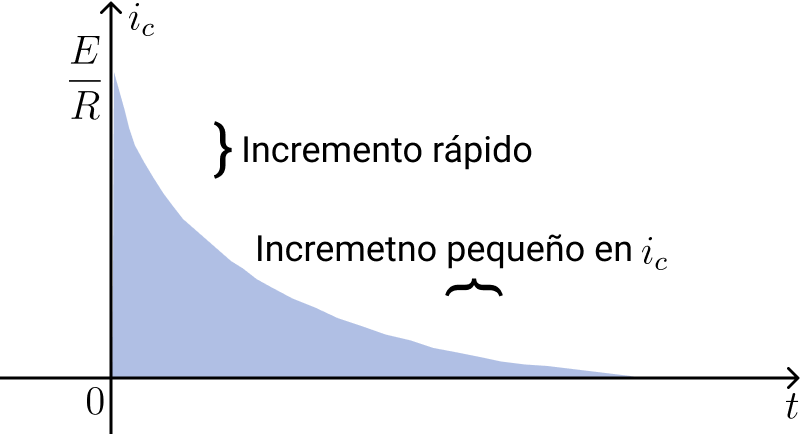
\includegraphics[width=\linewidth]{fe9.png}
		\caption{$i_{c}$ durante la fase de carga.}
		\label{fe9}
	\end{subfigure}
	\begin{subfigure}[b]{0.4\linewidth}
		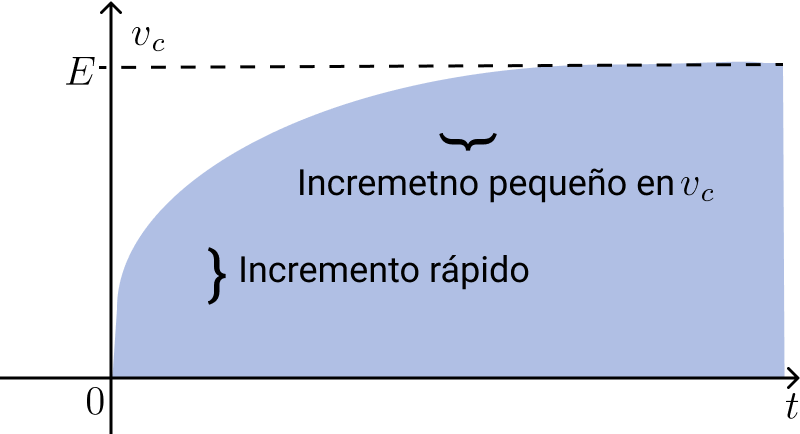
\includegraphics[width=\linewidth]{fe10.png}
		\caption{$v_{c}$ durante la fase de carga.}
		\label{fe10}
	\end{subfigure}
	\caption{Corriente y voltaje de los capacitores}
	\label{fig9-10}
\end{figure}


Un capacitor, se puede sustituir con un equivalente de circuito abierto una vez que ha pasado la fase de carga

\begin{center}
	\begin{circuitikz}[american]
		\draw (0,3) to [battery1=$E$](0,0);
		\draw (0,3) to [R=$R$, l_=$V_{R}{=}0V$](2,3);
		\draw (2,3) to (4,3);
		\draw (4,3) to [I, l_=$i_{C}{=}0A$, -*](6,3) to [open, v=$V_{C}{=}E$, -*](6,0) to (3,0) to [V<=12V,i=$0.125A$](0,0);
	\end{circuitikz}
\end{center}

Un capacitor es equivalente a un cortocircuito en $t=0$, cuando el interruptor esta en la posición número uno.

\begin{center}
	\begin{circuitikz}[american]
		\draw (0,3) to [battery1=$E$](0,0);
		\draw (0,3) to [R=$R$, l_=$V_{R}{=}E^{-}$](2,3);
		\draw (2,3) to (4,3);
		\draw (4,3) to [I, l_=$i_{R}{=}\frac{E}{R}$, -*](6,3) to [open, v=$V_{C}{=}0$, -*](6,0) to (3,0) to (0,0);
	\end{circuitikz}
\end{center}

El factor $e^{\frac{-t}{RC}}$ es una función exponencial de la forma $e^{-x}$, donde $x=\frac{-t}{RC}$ y $e=2.728281$,
El factor $RC$ en la ecuación se denomina constante de tiempo, su simbolo es $\tau$ (tau) y su unidad de medida es el segundo $s$
\begin{equation}
	\tau = RC
\end{equation}

\section{Fase de descarga en capacitores}

\begin{tikzpicture}[american]
	\draw (0,3) to [battery1=$E$](0,0);
	\draw (2,3) to [short, *-, l_=$1$](0,3);
	\draw (3,3) to [short, *-](4,3);
	\draw (3,3) to (2,4);
	\draw (3,0) to [short, -*, l_=$2$] (3,1.5);
	\draw (6,3) to (6,0);
	\draw (4,3) to [R=$R$, v=$v_{R}{=} 0$](6,3) to [curved capacitor=$E$,v=$v_C$ ](6,0) to (3,0) to (0,0);
	\draw [->,>=stealth] (8,1.5) -- (9,1.5);
	\draw (10,0) to [short, -*, l_=2](10,2);
	\draw (10,3)to [R=$R$, I=$i{=}0$, *-](12,3);
	\draw (10,3) to (9,4);
	\draw(12,3) to [curved capacitor=$V_{c}$](12,0);
	\draw (12,0) to (10,0);
\end{tikzpicture}

Para encontrar el voltaje en el capacitor de descarga:

\begin{align*}
	 & V_{c}=-V_{R}                              &  & \ln (V_{c})= \frac{t}{-RC}+K                                     \\
	 & V_{c}=-R\cdot C \frac{dv}{dt}             &  & e^{ln(V_{c})}=e^{\frac{t}{-RC}+k}=e^{\frac{t}{-RC}+k}\cdot e^{k} \\
	 & \frac{dv}{vc}=\frac{dt}{-R\cdot C}        &  & V_{c}=ke^{\frac{t}{-RC}}; t=0, V_{c}=E                           \\
	 & \int \frac{dv}{v_{c}}=\int \frac{dt}{-RC} &  & V_{c}=Ee^{\frac{-t}{RC}}
\end{align*}

Y luego para encontrar el voltaje se deriva:
\begin{align*}
	 & V_{c} & =Ee^{\frac{-t}{RC}} & i_{c} & = \frac{E}{R} e^{\frac{-t}{RC}} \\
	 & V_{c} & =-V_{r}
\end{align*}

\begin{figure}[h!]
	\centerline{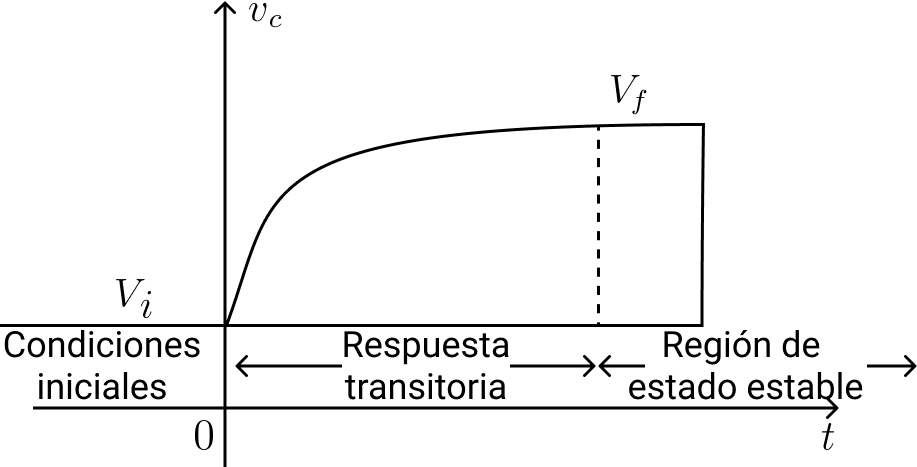
\includegraphics[width=0.7\textwidth]{fe13.png}}
	\caption{Valores iniciales}
	\label{fe13}
\end{figure}

\begin{equation}
	\text{Valores iniciales } V_{c}=V_{f}+\left( V_{i}-V_{f} \right) e^{- \frac{t}{\tau}}
\end{equation}

\subsection{Expresión matemática para la corriente}

La corriente pico resultante es:

\begin{equation}
	I_{m}=\frac{E-V_{c}}{R_{1}+R_{2}}
\end{equation}

\subsection{Inductores}

\begin{definition}[Inductores]
	Son bobinas de dimensiones diversas diseñadas par aintroducir cantidades especificas de inductancia dentro de un circuito. La inductancia de una bobina varia directamente con las propiedades magnéticas de esta
	\begin{equation}
		L=\frac{N^2 \mu A}{l}
	\end{equation}
	Donde $N$ representa el numero de vieltas, $\mu$ la permeabilidad del núcleo, $A$ el área del núcleo en metros cuadrados y $l$ la longitud media del núcleo en metros
\end{definition}

\begin{figure}[h!]
	\centerline{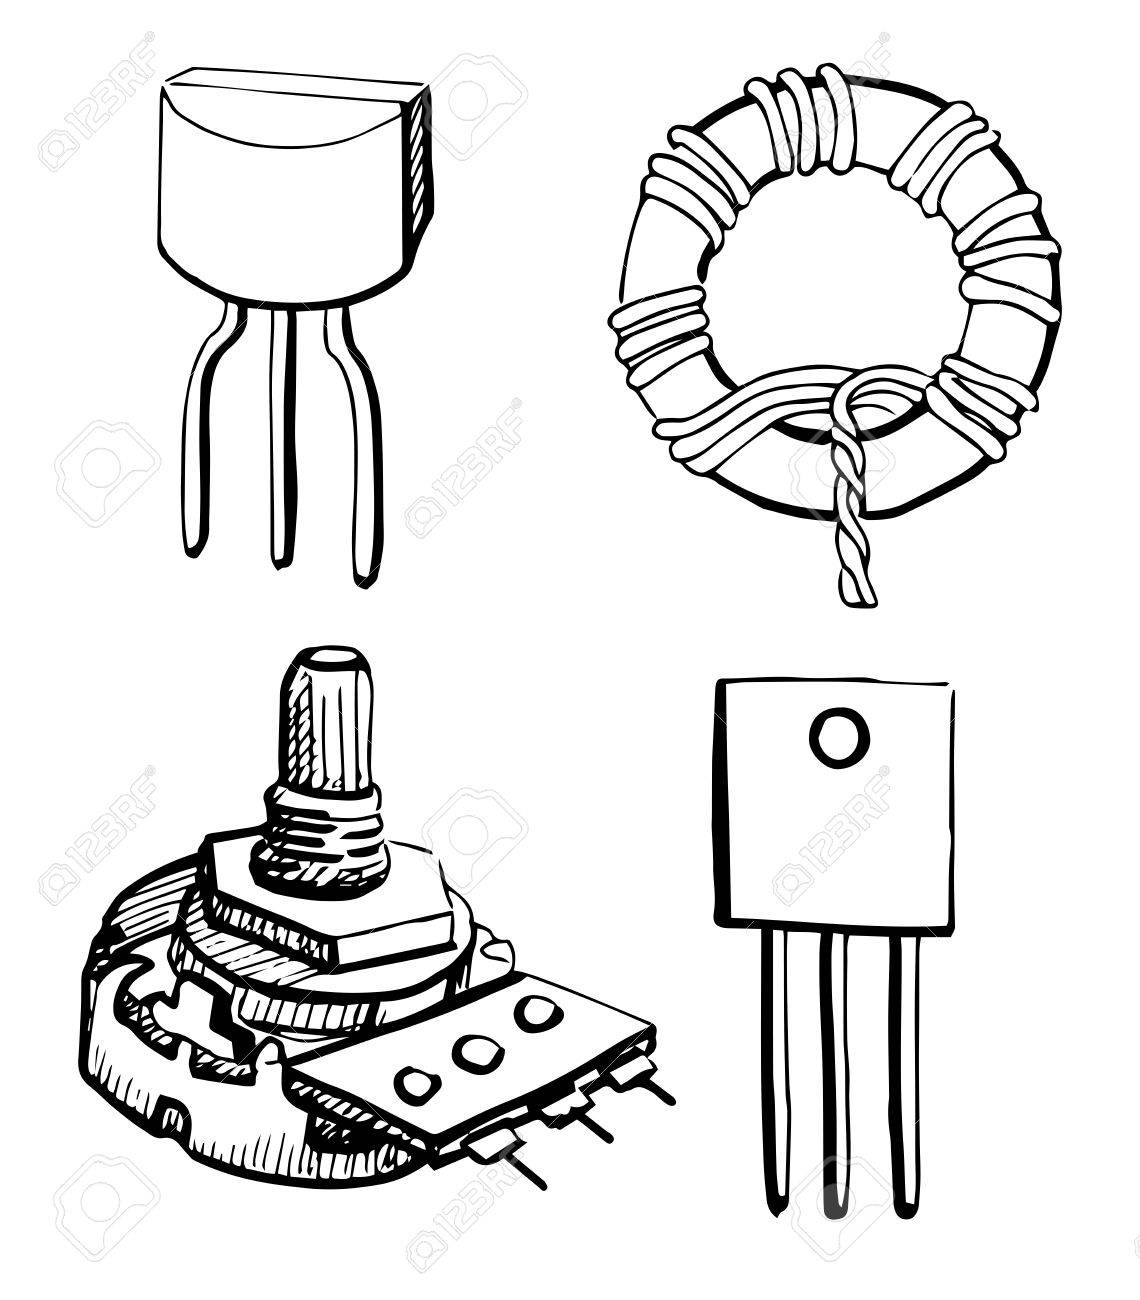
\includegraphics[width=0.25\textwidth]{fe11.jpg}}
	\caption{Inductores.}
	\label{fe11}
\end{figure}

%%%%%%%%%%%%%%%%%%%%circuito aquí casi listo ?

\section{Circuitos RL}

\begin{center}
	\begin{tikzpicture}[american]
		\draw (0,3) to [battery1=$E$](0,0);
		\draw (2,3) to (0,3);
		\draw (4,3) to [opening switch](2,3);
		\draw (4,3) to [R=$v_{R}$, v=$R$](6,3) to [cute inductor=$v_L$,v=$L$ ](6,0) to (3,0) to (0,0);
	\end{tikzpicture}
\end{center}

Deducción de la formula:
\begin{align*}
	 & V_{R}+V_{L}=E                          \\
	 & Ri+L \frac{di}{dt}=E                   \\
	 & \frac{di}{dt}+\frac{Ri}{L}=\frac{E}{L}
\end{align*}

Factor integrador

\begin{align*}
	 & e^{\int \frac{R}{L}dt}=e^{\frac{R}{L}t}                                                  &  & i=\frac{E}{R}+Ke^{\frac{-R}{L}t}; t=0, i=0                                                     \\
	 & e^{\frac{R}{L}t}+\frac{di}{dt}+^{\frac{R}{L}t} \frac{Ei}{L}=e^{\frac{R}{L}t} \frac{E}{L} &  & 0=\frac{E}{R}+Ke^{\frac{-R}{L}0}\implies k= -\frac{E}{R}                                       \\
	 & \frac{d}{dt}i\cdot e^{\frac{R}{L}t}=e^{\frac{R}{L}t}\frac{E}{L}                          &  & i=\frac{E}{R}-\frac{E}{r}e^{\frac{-R}{L}0}=\frac{E}{R}\left( 1-e^{\frac{-R}{L}t} \right)       \\
	 & \int \frac{d}{dt}i\cdot e^{\frac{R}{L}t}= \int e^{\frac{R}{L}t} \frac{E}{L} dt           &  & V_{r}=iR=R \frac{E}{R} \left( 1-e^{\frac{-R}{L}t} \right)=E \left( 1-e^{\frac{-R}{L}t} \right) \\
	 & i\cdot e^{\frac{R}{L}t}=e^{\frac{R}{L}t}\frac{E}{R}+K                                    &  & V_{L}=L \frac{di}{dt}=E\left(e^{\frac{-R}{L}t} \right)
\end{align*}

\subsubsection{Voltaje inducido y trnasistor RL: ciclo de almacenamiento}

\begin{equation}
	v_{L}=L \frac{di}{dt}
\end{equation}

Al instante que el circuito cierra el interruptor, entonces:

\begin{center}
	\begin{tikzpicture}[american]
		\draw (0,3) to [battery1=$E$](0,0);
		\draw (0,3) to [R=$R$, v=$v_{R}{=}iR{=}0R{=}0V$](3,3);
		\draw (3,3) to [I=$i_L{=}0A$](6,3) to [open, *-*, v=$V_L{=}E$](6,0) to (3,0) to (0,0);
	\end{tikzpicture}
\end{center}

Bajo condiciones estables:

\begin{center}
	\begin{tikzpicture}[american]
		\draw (0,3) to [battery1=$E$, i=$i$](0,0);
		\draw (0,3) to [R=$v_{R}{=}iR{=}\frac{E}{R}{=}E$, v=$R$](3,3);
		\draw (3,3) to [I=$i_L{=}\frac{E}{R}$](6,3) to [short,*-*, V=$V_L{=}0V$](6,0) to (3,0) to (0,0);
	\end{tikzpicture}
\end{center}

\subsection{Fase de caída}

\begin{center}
	\begin{tikzpicture}[american]
		\draw (0,3) to [battery1, l_=$E{=}50v$](0,0);
		\draw (2,3) to [short, *-](0,3);
		\draw (3,3) to [short, *-](4,3);
		\draw (3,3) to (2,4);
		\draw (3,0) to [short, -*, R=$R_{2}{=}3k\Omega$] (3,3);
		\draw (4,3) to [R=$R_{2}{=}3k\Omega$](6,3) to [cute inductor=$L$,v=$4H$ ](6,0) to (3,0) to (0,0);
	\end{tikzpicture}
\end{center}

\begin{align*}
	 & V_{L}+V_{R}=0 \implies L\frac{di}{dt}+iR=0                                  &  & \ln \left\lvert i \right\rvert  = -\frac{R}{L}t+C \implies i=Ce^{-\frac{R}{L}t}i(0)=i_{0}   \\
	 & \frac{di}{i}=-\frac{R}{i}dt \implies \int \frac{di}{i}=-\frac{R}{L} \int dt &  & \therefore i=i_{0}e^{-\frac{R}{L}t}, V_{L}=V_{0}e^{-\frac{R}{L}t}, V_{R}=Ee^{-\frac{R}{L}t}
\end{align*}

\begin{enumerate}
	\item Encuentre las expresiones matemáticas para $i_{L},V_{L},V_{R1}, V_{R2}$ para cinco constantes de tiempo de la fase de almacenamiento.
	\item Encuentre las expresiones matemáticas para $i_{L},V_{L},V_{R1}, V_{R2}$ si el interruptor se abre después de cinco constantes de tiempo de la dase de almacenamiento.
\end{enumerate}

\textit{ Sol. }

\begin{enumerate}
	\item
	      \begin{align*}
		       & v_{L}=Ee^{\frac{-t}{\tau}}                       &  & I_{m}=\frac{E}{R_{1}}=\frac{50V}{2k\Omega}=25mA                        \\
		       & v_{L}=50e^{\frac{-t}{\tau} \times 10^{-3}}       &  & I_{L}= 25\times 10^{-3} \left( 1-e^{\frac{-t}{2\times10^{-3}}} \right) \\
		       & i_{L}=I_{m} \left( 1-e^{\frac{-t}{\tau}} \right) &  & V_{R_{1}}=E \left( 1-e^{\frac{-t}{\tau}} \right)                       \\
		       &                                                  &  & V_{R_{2}}=50V
	      \end{align*}

	\item \begin{align*}
		       & v_{L}=- \left( V_{R_{1}}+V_{R_{2}} \right)=-\left( i_{1}R_{1}+i_{2}R_{2} \right)                                                        \\
		       & =-i_{L}\left( R_{1}+R_{2} \right)=-\frac{E}{R_{1}} \left( R_{1}+R_{2} \right)=- \left( \frac{R_{1}}{R_{1}}+\frac{R_{2}}{R_{1}} \right)E \\
	      \end{align*}

	      \begin{equation}
		      v_{L}= -\left( 1+ \frac{R_{2}}{R_{1}}\right)E
	      \end{equation}

	      \begin{align*}
		       & \tau'= \frac{L}{R_{1}+R_{2}}E=                                      &  & i_{L}= \left(25\times 10^{-3}\right)2e^{\frac{-t}{0.8\times10{-3}}}              \\
		       & \left(1+\frac{3k\Omega}{2k\Omega}\right)50v=125v                    &  & v_{R1}=Ee^{\frac{-t}{\tau'}}=50e^{\frac{-t}{0.8\times10{-3}}}                    \\
		       & v_{L}=-V_{i}e^{-\frac{t}{\tau'}}=-125e^{\frac{-t}{0.8\times10{-3}}} &  & V_{R2}=-\frac{R_{2}}{R_{1}}Ee^{\frac{-t}{\tau'}}=                                \\
		       & I_{i}=I_{m}=\frac{E}{R_{1}}=\frac{50v}{2k\Omega}=25mA               &  & \frac{-3}{2}\left(50V\right)e^{\frac{t}{\tau'}}-75e^{\frac{-t}{0.8\times10{-3}}}
	      \end{align*}
\end{enumerate}

\begin{figure}[h!]
	\centerline{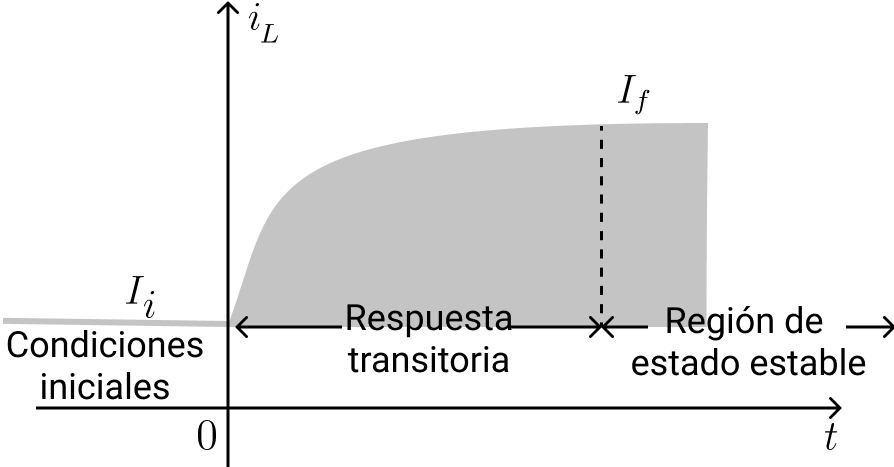
\includegraphics[width=0.7\textwidth]{fe12.png}}
	\caption{Valores iniciales}
	\label{fe12}
\end{figure}


\begin{equation}
	i_{L}=I-{f}+\left(I_{i}-I_{f}\right)e^{\frac{t}{\tau}}
\end{equation}


\begin{problem}[Encuentre las expresiones matemáticas] para el comportamiento transitorio de $i_{L}$ y $v_{L}$ para el circuito de la figura después de cerrar el interruptor.
\begin{center}
	\begin{tikzpicture}[american]
		\draw (0,3) to [battery1, l_=$E{=}50v$](0,0);
		\draw (2,3) to [short, *-](0,3);
		\draw (3,3) to [short, *-](4,3);
		\draw (3,3) to (2,4);
		\draw (4,3) to [R=$R_{1}{=}2k\Omega$](6,3) to [cute inductor=$L$,v=$4H$ ](6,0) to (3,0) to (0,0);
	\end{tikzpicture}
\end{center}

\textit{ Sol. }

Resolvemos la parte inicial:
\begin{align*}
	 & \tau=\frac{L}{R_{1}}=\frac{4H}{2k\Omega}=2ms                    &  & i_{L}=\left(25\times 10^{-3}\right)\left(1-e^{\frac{-t}{2\times 10{-3}}}\right) \\
	 & I_{m}=\frac{E}{R_{1}}=\frac{50}{2k\Omega}=25\times10^{-3}A=25mA &  & v_{L}=50e^{\frac{-t}{2\times 10^{-3}}}                                          \\
	 & i_{L}= \left(25.10^{-3}A\right)=25mA
\end{align*}
\end{problem}

\begin{problem}[El indcutor] de la figura tiene un nivel inicial de corriente de 4mA en la dirección mostrada
\begin{enumerate}
	\item Encuentre la expresión matemática para la corriente a través de la bobina una vez que se cierra el interruptor
	\item Encuentre la expresión matemática para el voltaje en la bobina nte el mismo periodo transitorio
\end{enumerate}
\begin{tikzpicture}[american]
	\draw (0,3) to [battery1, l_=$E{=}50v$](0,0);
	\draw (2,3) to [short, *-](0,3);
	\draw (3,3) to [short, *-](4,3);
	\draw (3,3) to (2,4);
	\draw (4,3) to [R=$R_{1}{=}2{.}2k\Omega$](6,3) to [cute inductor=$L{=}100mH$,v=$4H$ ](6,0) to (3,0) to [R=$R_{2}{=}6{.}8k\Omega$](0,0);
\end{tikzpicture}
\end{problem}

\textit{ Sol. }

\begin{equation*}
	I_{f}=\frac{E}{R_{1}+R_{2}}=\frac{16V}{2.2k\Omega+6.8k\Omega}= \frac{16V}{9k\Omega}=1.78mA
\end{equation*}
La constante de tiempo está determinada por:
\begin{align*}
	 & \tau=\frac{L}{R_{T}}=\frac{100mH}{2.2k\Omega+6.8k\Omega}=\frac{100mH}{9k\Omega}=11.11\mu s \\
	 & i_{L}=I_{f}+\left(I_{i}-I_{f}\right)e^{\frac{-t}{11.11\mu s}}                              \\
	 & =1.78mA+2.22mAe^{\frac{-t}{11.11\mu s}}
\end{align*}

como la corriente a través del inductor es de 4ma antes del cierre del interruptor, el voltaje (cuyo nivel es sensible solo a cambios en la corriente a través de la bobina) debe tener un valor inicial de $0V$. Al momento en que el interruptor se cierra, la corriente a través de la bobina no puede cambiar instantaneamente, por lo que la corriente de los elementos resistivos será de 4mA. EL voltaje pico resultante en $t=0s$ puede entonces encontrarse usando la ley de voltaje de Kirchhoff como sigue:
\begin{align*}
	 & V_{m}=E-V_{R1}-V_{R2}                                                                  \\
	 & =16V-\left(4mA\right)\left(2.2k\Omega\right)- \left(4mA\right)\left(6.78k\Omega\right) \\
	 & =16V-8.8V-27.2V=16V-36V                                                                \\
	 & =-20V
\end{align*}
La ecuación para $V_{L}$ por lo tanto: $v_{L}=-20e^{\frac{-t}{11.11 \mu S}}$


\begin{problem}[Encontrar $i_{0}, V_{0, i}$] para todo momento. Asuma que el interruptor estuvo abierto por mucho tiempo

\begin{tikzpicture}[american]
	\draw (0,0) to[V=$10V$] (0,3) to
		[R=$2\Omega$](2,3) to[short,l_=$t{=}0$](2,1.5);
	\draw (2,1.5) to (1,1);
	\draw (2,0) to (2, 1);
	\draw (2,0) to (0,0);
	\draw (2,3) to [R=$3\Omega$, v=$v_{0}$](4,3) to[R=$6\Omega$,i=$i_{0}$](4,0) -- (2,0);
	\draw(4,3) to [I=$i$](6,3) to[cute inductor=$2H$] (6,0) to (4,0);
\end{tikzpicture}
\end{problem}

\textit{ Sol. }

Es mejor calcular primero $i$ y luego las otras cantiades. Para $i<0$, el interruptor está abierto. EL inductor actúa como un cortocircuito en corriente directa, el resistor de $6\Omega$ está en ocorto y queda el circuito siguiente:
\begin{align*}
	 & \therefore i_{0}=0                           \\
	 & i(t)=\frac{v}{R}=\frac{10V}{5\Omega}=2A, t<0
\end{align*}

Para $t>0$ el interruptor se cierra, por lo que la fuente de voltaje queda en cortocircuito. Por lo que se tiene un circuito RL sin fuente como a continuación:
\begin{center}
	\begin{tikzpicture}[american]
		\draw (0,0) to[battery1] (0,3) to [R=$3\Omega$, v=$V_{0}$](2,3);
		\draw (2,3) -- (4,3) to[R=$6\Omega$, i=$I_{0}$](4,0);
		\draw(4,3) to [I=$i$](6,3) to[cute inductor=$2H$, v=$v_{L}$] (6,0) to (0,0);
	\end{tikzpicture}
\end{center}
Calculamos la resistencia equivalente de Thevein en las terminales del inductor.
$R_{th}= 3 \mid \mid 6=2\Omega$ por lo que la constante del tiempo es $\tau=\frac{L}{R_{th}}=1s$
Por lo tanto $i(t)=i(0)e^{\frac{-t}{\tau}}=2e^{-t}$
Puesto que el inductor está en paralelo con las resistencias de $6\Omega$ y $3\Omega$
\begin{align*}
	 & i(t)=i(0)e^{\frac{-t}{\tau}}=2e^{-t}                                       \\
	 & v_{0}(t)=-v_{L}=-L\frac{di}{dt}=-2\left(-2e^{-t}\right)=4e^{-t}            \\
	 & i_{0}(t)= \frac{V_{L}}{6\Omega}=\frac{4e^{-t}}{6\Omega}=-\frac{2}{3}e^{-t}
\end{align*}

Por lo tanto, para cualquier momento:

\begin{align*}
	 & \schema{\schemabox{$i_{0}(t)$}}{\schemabox{$0A$ \\ $-\frac{2}{3}e^{-t}A$}} &&
	\schema{\schemabox{$t>0$                           \\ $t<0$}}{} && \schema{\schemabox{$v_{0}(t)$}}{\schemabox{$6V$ \\ $4e^{-t}V$}} && &&
	\schema{ \schemabox{$t>0$                          \\ $t<0$}}{} \\
	\schema{\schemabox{$i(t)$}} {\schemabox{$2A$       \\ $2e^{-t}A$}} &&
	\schema{\schemabox{$t>0$                           \\ $t\geq0$}}{}
\end{align*}

\subsection{Inductores en serie y paralelo}

\subsubsection{Serie}

\begin{tikzpicture}[american]
	\draw (0,0) to[short, open, *-*, v=$v$] (0,3) to [cute inductor=$L_1$, v=$v_1$](2,3);
	\draw (2,3) to [cute inductor=$L_2$, v=$v_2$](4,3);
	\draw(4,3) to [cute inductor=$L_N$, v=$v_N$](6,3) to(6,0) to (0,0);
\end{tikzpicture}

\begin{equation}
	v=v_{1}+v_{2}+v_{3}+\dots +v_{n}
\end{equation}

\begin{equation}
	\left(L_{1}+L_{2}+L_{3}+\dots +L_{N}\right)\frac{di}{dt}
\end{equation}

\begin{equation}
	\left(\sum_{k=1}^{N}\frac{di}{dt}\right)=L_{eq}\frac{di}{dt}
\end{equation}

\begin{equation}
	L_{eq}=L_{1}+L_{2}+L_{3}+\dots+ L_{N}
\end{equation}

\subsubsection{Paralelo}

\begin{center}
	\begin{tikzpicture}[american]
		\draw (0,3) to[short, open, v=$v$, *-*] (0,0);
		\draw (0,3) to [I=$i$](2,3) to[cute inductor =$L_{1}$, i=$i_{1}$] (2,0) -- (0,0);
		\draw (2,3) to [I=$i_{2}$](4,3) to[cute inductor=$L_{2}$](4,0) to (2,0);
		\draw(4,3) to [I=$i_{3}$](6,3) to[cute inductor=$L_{3}$](6,0) to (4,0);
		\draw (6,3) to [I=$i_{N}$](9,3) to [cute inductor=$L_{N}$](9,0) to (6,0);
	\end{tikzpicture}
\end{center}

\begin{align*}
	 & i=i_{1}+i_{2}+i_{3}\dots i_{N}                                                                                                                                                                        \\
	 & i_{k}=\frac{L}{L_{1}}\int_{t_{0}}^{t}v dt +i_{i}\left(t_{0}\right)+\frac{1}{L_{2}}\int_{t_{0}}^{t}v dt + i_{2}\left(t_{0}\right)+\dots +\frac{1}{L_{N}}\int_{t_{0}}^{t}v dt + i_{N}\left(t_{0}\right) \\
	 & =\left(\frac{1}{L_{1}}+\frac{1}{L_{2}}+\dots \frac{1}{L_{N}}\right)\int_{t_{0}}^{t}v dt + i_{1}\left(t_{0}\right)+i_{2}\left(t_{0}\right)+i_{N}\left(t_{0}\right)                                     \\
	 & \left(\sum_{K=1}^{N} \frac{1}{L_{k}} \right)\int_{t_{0}}^{t}v dt+\sum_{K=1}^{N} i_{K}\left(t_{0}\right)=\frac{1}{L_{eq}}\int_{t_{0}}^{t}v dt+i\left(t_{0}\right)
\end{align*}


\begin{equation}
	\frac{1}{L_{eq}}=\frac{1}{L_{1}}+\frac{1}{L_{2}}+\frac{1}{L_{3}}+ dots +\frac{1}{L}
\end{equation}


\begin{example}
	Para el circuito mostrado a continuación $i(t)=4(2-e^{-10t})mA$ si $i_{2}(0)=-mA$ Encontrar $i_{1}(0), v(t), v_{1}(t),v_{2}(t), i_{1}(t),i_{2}(t)$
\end{example}
\begin{tikzpicture}[american]
	\draw (0,3) to[short,open, *-*, v=$v$] (0,0);
	\draw (0,3)to [I=$i$](2,3) to [cute inductor =$2H$,v=$v_{1}$](4,3);
	\draw (2,3) to [short, -*](4,3) to[cute inductor =$4H$,-*,i=$i_{1}$, ] (4,0);
	\draw(4,3) to (6,3) to[cute inductor =$12H$, i=$i_{2}$, v=$v_{2}$] (6,0) to (0,0);
\end{tikzpicture}
\textit{ Sol. }

\begin{align*}
	 & V_{R}=i_{R}               &  & V_{1}=2\left(40e^{-10t}\right)=80e^{-10t}                   \\
	 & i=8-4e^{-10t}             &  & V_{2}=V-V_{1}=120e^{-10t}                                   \\
	 & E-V_{a}-V_{b}=0           &  & v=L \frac{di}{dt}                                           \\
	 & E_iR-L \frac{di}{dt}=0    &  & \int \frac{di}{dt}                                          \\
	 & V_{L}=L_{eq}\frac{di}{dt} &  & \int di=\frac{120}{4}\int e^{-10t}dt+5H                     \\
	 & i_{1}=i-i_1            &  & -3e^{-10t} \left.\begin{matrix} t\\ 0 \end{matrix}\right|+5 \\
	 & i(0)=4-(-1)=5mA           &  & -3e^{-10t}-(-3)+5                                           \\
	 & L_{eq}=5H                 &  & 8-3e^{-10t}                                                 \\
\end{align*}

\begin{example}
	Para el circuito mostrado a continuación $i_{1}(t)=0.6e^{-2t}A$ si $i(0)=1.4A$, encontrar $i_{2}(0), i_{2}(t), i(t)$ y $v_{1}(t),v_{2}(t),v(t)$
	\begin{tikzpicture}[american]
		\draw (0,3) to [open, *-*,v=$v$](0,0);
		\draw (0,3) to [I=$i$](2,3);
		\draw (2,4) to [cute inductor=$3H$,i=$i_{2}$, v=$v_{1}$](4,4);
		\draw (4,4) to (4,2);
		\draw (2,2) to [cute inductor=$6H$, i=$i_{1}$](4,2);
		\draw (2,2) to (2,4);
		\draw (4,3) to (5,3) to (6,3) to [cute inductor=$8H$, v=$v_{2}$](6,0);
		\draw (0,0) to (5,0) to (6,0);
	\end{tikzpicture}
\end{example}

\textit{ Sol. }
%%%%%%%%%%%%%%%%%%%%%%%%%%%%%%%%%%%%%%%%%%%%%%%%%

\begin{problem}
El interruptor en el circuito ha estado cerrado por mucho tiempo.
En $t=0$ el interruptor se abre. Calcule $i(t)$ para $t>0$\\
\begin{tikzpicture}[american]
	\draw (-1,0) to[battery1=$40V$] (-1,3) to [R=$2\Omega$](1,3) to
	[opening switch](3,3);
	\draw (2,3) to[R=$12\Omega$](2,0) -- (-1,0);
	\draw (3,3)to [R=$4\Omega$](5,3) to[R=$16\Omega$](5,0) -- (2,0);
	\draw(5,3) to (7,3) to[cute inductor=$2H$, i=$i_{t}$] (7,0) to (5,0);
\end{tikzpicture}
\end{problem}
\textit{ Sol. }
%%%%%%%%%%%%%%%%%%%%%%%%%%%%%%%%%%%%%%%%%%%%%

\section{Corriente alterna}

Los voltajes senoidales de $ca$ están disponibles a partir de una diversidad de fuentes.

\begin{definition}[Amplitud pico]
	Valor máximo de una fomra de onda medido a aprtir de su valor promedio o medio, denotado por letras mayúsculas (como $E_{m}$ para fuentes de voltaje y $V_{m}$ para la caída de voltaje en la carga).
	Para la forma de onda de la figura anterior, el valor promedio es cero volts, y $E_{m}$ es como lo define la figura.
\end{definition}

\begin{definition}[Forma de onda periódica]
	Es la forma de onda que se repite continuamente después del mismo intervalo de tiempo
\end{definition}

\begin{definition}[Periodo $T$]
	Inervalo de tiempo entre repeticiones sucesivas de una forma de onda periódica (el periodo $T_{1}=T_{2}=T_{3}$ en la figura ), siempre que puntos similares sucesivos de la forma de onda periódica se utilicen para determinar $T$.
\end{definition}

\begin{definition}[Ciclo]
	Parte de una forma de onda contenida en un periodo
\end{definition}

\begin{definition}[Frecuencia ($f$)]
	Número de ciclos que suceden en un segundo
\end{definition}
La unidad de medición para la frecuencia es el Hertz $(Hz)=1$ ciclo por segundo $c/s$
\begin{equation}
	f=\frac{1}{T}
\end{equation}
Donde $f=Hz$ y Y $T=\text{segundos}(s)$

\begin{example}
	Encuentre el periodo de una forma de onde periódica con una frecuencia de 60$Hz$ y $100Hz$
	\textit{ Sol. }

	\begin{enumerate}
		\item $T=\frac{1}{f}=\frac{1}{60Hz}=16.36ms$
		\item $T=\frac{1}{f}=\frac{1}{1000Hz}=0.001s$
	\end{enumerate}
\end{example}

La onda senoidal es la única forma de onda alterna cuyo aspecti no se ve afectado por las características de un resistor, inductor o capacitor puro.
\begin{equation}
	\text{Radianes}= \frac{\pi}{180^{\circ}}\times \text{grados}
\end{equation}

\begin{equation}
	\text{Velocidad angular}= \frac{\text{Distancia (ágnulo)}}{\text{Tiempo (segundos)}}
\end{equation}

%%%%%%%%%%%%%%%%%%%%%%%%%%%%%%%%%%%%%%%%%%%%%%%%%



\begin{definition}[Fase de una corriente eléctrica]

\end{definition}

\begin{definition}[Mediciones RMS]

\end{definition}

%%%%%%%%%%%%%%%%%%%%%%%MUCHAS GRAFICAS DESPUéS

\subsection{Valores efectivos (rms)}

Relacionan las cantidades de $cd$ y $ca$ con la potencia entregada a una carga. SIe el interruptor dos, se
cierra y el interruptor uno se mantiene abierto, la corriente de $ca$ a través del resitor tendrá un valor pico de $Im$.
La temperatura alcanzada entonces por el agua es determinada por la potencia de $ca$ disipada en forma de claor por el resistor.

%%%%%%%%%%%%circuito complejo aquí

\begin{align*}
	P_{ca}=\left(i{ca}\right)^2R=\left(I_{m}\sin{\omega t} \right)R       \\
	\sin^2{\omega t}=\frac{1}{2}\left(1-\cos{2\omega t}\right)            \\
	P_{ca}=I_{m}^2\left(\frac{1}{2}\left(1-\cos{2\omega t}\right)\right)R \\
	P_{ca}=\frac{I_{m}^2R}{2}-\frac{I_{m}^2}{2}\cos{2\omega t}
\end{align*}

La potencia promedio entregada por la fuente de ca es únicamente el primer término:

\begin{align*}
	 & P_{\text{promedio (ca)}}=P_{cd}                   \\
	 & \frac{I^2_{m}R}{2}=I^2{cd}R, I_{m}=\sqrt{2I_{cd}} \\
	 & I_{cd}=\frac{I_{m}}{\sqrt{2}}=0.707I_{m}
\end{align*}

el valor equivalente de $cd$ de una corriente o un voltaje senoidales es $\frac{1}{\sqrt{2}}$ o 0.707 de su valor
máximo. El valor de $cd$ equivalente se denomina valor efectivo de la cantidad senoidal.

\begin{equation}
	I_{ec(cd)}=I_{efectivo}=0.0707I_{m}
\end{equation}

\begin{equation}
	I_{m}=\sqrt{2I{efectivo}}=1.414I_{efectivo}
\end{equation}

\subsubsection{Mediciones RMS}

Valor \textbf{RMS}. La cantidad de corriente alterna y voltajes (cuando son alternos) se
expresan de forma común por su valor efectivo o \textbf{RMS} (Root Mean Square - Raíz media cuadrática).
CUando se dice que en nuestras casas tenemos 120 o 220 voltios, éstos son valores RMS o eficaces.

\subsection{Respuesta de los elementos básicos E,L,C a un voltaje o una corriente senoidal}

\textbf{Resistor}

\begin{tikzpicture}
	\draw (0,0) to [short, open, *-*] (0,3) to [I=$i$](2,3);
	\draw (2,3)to [R=$R_{1}$, v=$v$](2,0) to (0,0);
\end{tikzpicture}

\begin{align*}
	 & i=\frac{v}{R}=\frac{V_{m} \sin(\omega t)}{R}=VI_{m} \sin(\omega t) &  & v=iR= I_{m}\sin(\omega t)R = I_{m} \sin(\omega t)=V_{m} \sin(\omega t) \\
	 & I_{m}=\frac{V_{m}}{R}                                              &  & V_{m}=I_{m}R
\end{align*}

Para un elemento puramente resistivo, el voltaje y la corriente a través del elemento se encuentran en fase, con sus valores pico relacionados mediante la ley de Ohm.

\begin{equation}
	v_{L}=L \frac{di_{L}}{dt}
\end{equation}

y al aplicar diferenciación:

\begin{align*}
	 & \frac{di_{L}}{dt}=\frac{d}{dt}\left(I_{m}\sin{\omega t}\right)=\omega I_{m}\cos{\omega t}     \\
	 & v_{L}=L\frac{di_{L}}{dt}=L\left(\omega I_{m}\cos{\omega t}\right)=\omega LI_{m}\cos{\omega t} \\
	 & v_{L}=V_{m}\sin{\omega t+ 90^{\circ}}                                                         \\
	 & v_{m}=\omega LI_{m}                                                                           \\
\end{align*}

Para un inductor, $v_{L}$ adelanta a $i_{L}$ por $90^{\circ}$, o está retrasada con respecto a $v_{L}$
por $90^{\circ}$.

Si un ángulo de fase está incluido en la expresión senoidal de $I_{L}$, tal como:

\begin{align*}
	 & i_{L}=I_{m}\sin{\omega t \pm \theta}                      \\
	 & v_{L}=\omega LI_{m}\sin{\omega t \pm  \theta 90^{\circ}+}
\end{align*}

\subsubsection{Reactancia}

\begin{equation}
	X_{L}=\omega L
\end{equation}

\begin{equation}
	X_{L}=\frac{V_{m}}{I_{m}}
\end{equation}

\textbf{Capacior}

\begin{equation}
	i_{c}=C \frac{dv_{c}}{dt}
\end{equation}

Al aplicar diferenciación:

\begin{align*}
	 & \frac{dv_{c}}{dt}=\frac{d}{dt}\left( V_{m}\sin{\omega t} \right)=\omega V_{m}\cos{\omega t} \\
	 & i_{C}=C\frac{dv_{c}}{dt}=C\left( \omega V_{m}\cos{\omega t} \right)
\end{align*}


Para un capacitor en donde $i_{c}$ sobrepasa a $v_{c}$ por $90^{\circ}$ o $v_{c}$ se retrasa
por $90^{\circ}$ con respecto a $i_{c}$

La corriente de un elemento puramente capacitivo adelanta al voltaje en el elemento por $90^{\circ}$.

La cantidad $\frac{1}{\omega C}$, denominada la \textbf{reactancia} de un capacitor, se representa simbólicamente por $X_{C}$ y puede medirse en Ohms.

%OTRA GRAFICAAAAAAAAAAAA

\begin{equation}
	X_{C}=\frac{1}{\omega C}
\end{equation}

En formato de la ley de Ohm, su magnitud puede determinarse
\begin{equation}
	X_{C}=\frac{V_{m}}{I_{m}}
\end{equation}

\subsection{Vectores}

Forma rectangular:
%%%%%%%%%GRAFICAAAAAAAAAAAAAA
\begin{align}
	 & C=A+jB                                     \\
	 & \left\lvert C \right\rvert =\sqrt{A^2+B^2} \\
	 & \theta=\tan^{-1} \left( \frac{B}{A}\right)
\end{align}

Forma polar:

\begin{align*}
	 & C=\left\lvert C \right\rvert <\theta          \\
	 & A=C\times\cos{\theta} \times B=C \sin{\theta}
\end{align*}

\begin{example}
	\begin{equation*}
		C=\left\lvert 10 \right\rvert
	\end{equation*}
\end{example}

\textit{Sol. }
\begin{align*}
	 & A=10\cos{45}B=10\sin{45} \\
	 & C=7{.}07+j7{.}07
\end{align*}

\begin{example}
	\begin{equation*}
		C=-6+j3
	\end{equation*}
\end{example}

\textit{Sol. }

\begin{equation*}
	C=\left\lvert 6{.}7 \right\rvert  <
\end{equation*}

\begin{equation}
	C=-Z< \theta =Z< \theta \pm 180^{\circ}
\end{equation}

%%%%%%%%%%%%%GRAFICAAAAAAAAAAAAA

\begin{align}
	 & V=V_{m}<\phi &  & I_{m}<-\theta
\end{align}

\subsubsection{Suma}

\begin{enumerate}
	\item $C_{1}=2+4j4; + C_{2}=3+j1$
	\item $C_{1}=3+j6; + C_{2}=-6+j3$
\end{enumerate}

\textit{Sol. }

\begin{align*}
	 & C_{1}+C_{2}=\left(2+3\right)+j\left(4+1\right)=5+j5  \\
	 & C_{1}+C_{2}=\left(3-6\right)+j\left(6+3\right)=-3+j9
\end{align*}

\subsubsection{Resta}

\begin{equation}
	C_{1}-C_{2}=1\pm x_{2}-\left(\pm x_{2}\right)+j\left(\pm y_{1}-\left(\pm y_{2}\right)\right)
\end{equation}

\begin{enumerate}
	\item $C_{2}=2+j4; C_{1}=4+j6$
	\item $C_{2}=-2+j6; C_{1}=3+j3$
\end{enumerate}

\textit{Sol. }

\begin{align*}
	 & C_{1}-C_{2}=\left(4-1\right)+j\left(6-4\right)=3+j2 \\
	 & C_{1}-C_{2}=\left(3+2\right)+j\left(3-5\right)=5+j2
\end{align*}

La suma o la resta no podrá realizarse en forma polar a menos que los números complejos tengan el mismo ángulo o a menos que éstos difieran sólo por múltiplos de 180$^{\circ}$

\subsubsection{Multiplicación}

\begin{equation*}
	C_{1}=x_{1}+jy_{1}; C_{2}=x_{2}+jy_{2}
\end{equation*}

\begin{align*}
	 & C_{1}\cdot C_{2}=                                                  \\
	 & x_{1}+jy_{1}\cdot x_{2}+jy_{2}=                                    \\
	 & jx_{1}y_{2} \cdot j^2y_{1}y_{2}=                                   \\
	 & x_{1}x_{2}+j\left(x_{1}y_{1}x_{2}\right)+y_{1}y_{2}\left(-1\right)
\end{align*}

\begin{equation}
	C_{1}\cdot C_{2}=\left(x_{1}x_{2}-y_{1}y_{2}\right)+j\left(y_{1}x_{2}+x_{1}y_{2}\right)
\end{equation}

\subsubsection{Multiplicación polar}

En forma polar, las magnitudes se multiplican y los ángulos se suman de forma algebraica.

\begin{equation*}
	C_{1}=Z_{1}<\theta_{1}; C_{2}=Z_{2}<\theta_{2}
\end{equation*}
\begin{equation}
	C_{1}\cdot C_{2}=Z_{1}Z_{2}<\theta_{1}+\theta_{2}
\end{equation}

\subsubsection{División}
\begin{equation*}
	C_{1}=x_{1}+y_{2}; C_{2}=x_{2}+jy_{2}
\end{equation*}

\begin{equation}
	\frac{C_1}{C_2}=\frac{x_{1}x_{2}+y_{1}y_{2}}{x_{2}^2+y_{2}^2}+j \frac{x_{2}y_{1}-x_{1}y_{2}}{x_{2}^2+y_{2}^2}
\end{equation}

\subsubsection{División polar}

En forma polar, la división se logra dividiendo la magnitud del numerador entre la magnitud del denominador y restando el ángulo de denominador del ángulo del numerador:

\begin{equation*}
	C_{1}=Z_{1}<\theta_{1}; C_{2}=Z_{2}<\theta_{2}
\end{equation*}

\begin{equation}
	\frac{C_{1}}{C_{2}}=\frac{Z_{1}}{Z_{2}}<\theta_{1}-\theta_{2}
\end{equation}

\begin{table}[h!]
	\centering
	\begin{tabular}{|c|c|}
		\hline
		\textbf{Dominio del tiempo}   & \textbf{Dominio del Fasor} \\ \hline
		$V_{m}\cos(\omega t+\phi)$    & $V_{m}<\phi$               \\ \hline
		$V_{m}\sin(\omega t+\phi)-90$ & $V_{m}<\phi-90$            \\ \hline
		$I_{m}\cos(\omega t+\phi)$    & $I_{m}<\theta$             \\ \hline
		$I_{m}\sin(\omega t+\phi)-90$ & $I_{m}<\theta-90$          \\ \hline
	\end{tabular}
	\caption{Fasores, donde $\omega=2\pi f$}
	\label{tabelec3}
\end{table}

\subsection{Circuitos de ca en serie y en paralelo}

En forma fasorial

\begin{equation}
	v=V_{m}\sin (\omega t)\implies V=v<0
\end{equation}

Donde $V=0.707V_{m}$

Al aplicar la ley de Ohm y utilizar el álgebra fasorial, tenemos:

\begin{equation}
	I?\frac{V<0}{R<\theta_{R}}=\frac{V}{R}<0-\theta_{R}
\end{equation}

Dado que $i$ y $v$ están en fase, el ángulo asociado con $i$ también deberá ser 0. Para satisfacer esta condición, $\theta_{R}$
debe ser iguala  0. Al sustituir $\theta_{R}=0$, observamos:

\begin{equation}
	I=\frac{V<0}{R<0}=\frac{V}{R}<0-0=\frac{V}{R}<0
\end{equation}

Por lo que en el dominio del tiempo:

\begin{equation}
	i=\sqrt{2}\left(\frac{V}{R} \right)\sin(\omega t)
\end{equation}

\begin{equation}
	\text{Impedancia }Z_{R}=R<0
\end{equation}

Utilizando álgebra compleja, encuentre el voltaje para el circuito

\begin{center}
	\begin{tikzpicture}[american]
		\draw (0,0) to[open, *-*] (0,3) to [I=$I_{in}$, l_=$i{=}4\sin(\omega t+30)$](4,3);
		\draw (2,3) to [short, -*](4,3) to[R=$2\Omega$,-*,v=$v$] (4,0) to (0,0);
	\end{tikzpicture}
\end{center}

\begin{align*}
	 & i=4\sin(\omega t+30)\implies \text{Forma fasorial } I=2.82A<30 \\
	 & V=IZ_{R}=(I<\theta)(R<0)=(2.8228A<30)(2\Omega<0)=5.656V<30     \\
	 & v=\sqrt{2}(5.656)\sin(\omega t+30)=8\sin(\omega t +30)
\end{align*}

\subsection{Reactancia inductiva}

\begin{center}
	\begin{tikzpicture}[american]
		\draw (0,0) to[open, *-*] (0,3) to [I=$i$](4,3);
		\draw (2,3) to [short, -*](4,3) to[cute inductor=$X_{L}{=}\omega L$,-*,v=$v{=}V_{M}$] (4,0) to (0,0);
	\end{tikzpicture}
\end{center}

\begin{equation*}
	v=V_{M}\sin(\omega t)\implies \text{Forma fasorial } V=v<0
\end{equation*}

Mediante la ley de Ohm:

\begin{equation}
	I=\frac{V<0}{X_{L}<\theta_{L}}=\frac{V}{X_{L}}<0-\theta_{L}
\end{equation}

Dado que $v$ adelanta a $i$ por 90, $i$ debe tener un ángulo asociado de -90. Para satisfacer esta condición, $\theta_{L}$ deberá ser igual a 90. Al sustituir $\theta_L=90$, obtenemos:

\begin{equation*}
	I=\frac{V<0}{X_{L}<90}=\frac{V}{X_{L}}<0-90
\end{equation*}

Por lo que, en el dominio del tiempo

\begin{equation*}
	i=\sqrt{2}\left(\frac{V}{X_{L}} \right)\sin(\omega t-90)
\end{equation*}

El hecho de que $\theta_L=90$ se empleará en el siguiente formato de coordenadas polares de reactancia para asegurar la adecuada relación de dase entre el voltaje y la corriente de un inductor:

\begin{equation}
	Z_L=X_L<90
\end{equation}

%%%%%%%%%%%%%%%%%%%%%%%%%%%%%%%%%% OTRO PARECIDOOOOOOOOOOO

\subsection{Circuitos de ca en serie}

Para la configuración de un circuito de ca en seria, la corriente es la misma a través de cada elemento:

\begin{align*}
	 & Z_T=Z_{1}+Z_{2}   &  & V_{1}=IZ_1 &  & E=V_{1}-V_{2}=0 \\
	 & I=\frac{E}{Z_{T}} &  & V_{2}=IZ_2 &  & E=V_{1}+V_{2}
\end{align*}

La potencia al circuito se puede determinar mediante:

\begin{center}
	\begin{tikzpicture}[american]
		\draw (0,0) to [sV=$E$, l_=$Z_{T}$] (0,3) to  (2,3) ;
		\draw (2,3) to [european resistor=$Z_{1}$, v=$V_{1}$](4,3);
		\draw (4,3) to (6,3) to [european resistor=$Z_{2}$, v=$V_{2}$](6,0) to (0,0);
	\end{tikzpicture}
\end{center}

\begin{equation}
	P=EI\cos(\theta_{T})
\end{equation}


En notación fasorial tenemos que:

\begin{equation*}
	e=141.4\sin(\omega t)\implies E=100V<0
\end{equation*}


\begin{example}
	Calcular $V_{R}, V_{L}, ci$ para el siguiente circuito:

	\begin{center}
		\begin{circuitikz}[american]
			\draw (0,0) to [sV=$e{=}141.4\sin(\omega t)$](0,3) to [R=$3\Omega$, v=$v_R$] (2,3) ;
			\draw (2,3) to (4,3);
			\draw (4,3) to [cute inductor=$X_L{=}4\Omega$, v=$v_L$](6,3) to [I=$i$](6,0) to (0,0);
		\end{circuitikz}
	\end{center}

\end{example}

Para calcular $Z_T$:
\begin{align*}
	 & Z_T=Z_1+Z_2=3\Omega<0+4\Omega<90=3\Omega+j4\Omega       \\
	 & Z_T=5\Omega <53.13                                      \\
	 & I=\frac{E}{Z_T}=\frac{100V0}{5\Omega 53.13}=20A< -53.13
\end{align*}


\textit{Sol. }

para encontrar $V_R$ y $V_L$ se aplica:

\textbf{Ley de Ohm}

\begin{align*}
	 & V_R=IZ_R=\left(20A < -53.13\right)\left(3\Omega <0\right)  \\
	 & =60V < -53.13                                              \\
	 & V_L=IZ_L=\left(20A < -53.13\right)\left(4\Omega <90\right) \\
	 & =80V<36.87
\end{align*}

\textbf{Ley de voltaje de Kirchhoff}

\begin{align*}
	 & \sum V=E-V_R-V_L=0       \\
	 & E=V_0+V_1                \\
	 & V_R=60V< -53.13=36V-j48V \\
	 & V_L=80V<+36.87=64V+j48V
\end{align*}

\begin{equation*}
	E=V_R+V_L=\left(36V-j48V\right)+\left(64V+j48V\right)=100V+j0=100V<0
\end{equation*}


\begin{problem}[Calcular $V_R$ y $V_C$]
\begin{center}
	\begin{circuitikz}[american]
		\draw (0,0) to [I, l_=$i{=}7.07\sin(\omega t+53.13)$](0,3) to [R=$R{=}6\Omega$, v=$v_R$] (2,3) ;
		\draw (2,3) to (4,3);
		\draw (4,3) to [curved capacitor=$X_C{=}8\Omega$, v=$v_C$](6,3) to [I=$i$](6,0) to (0,0);
	\end{circuitikz}
\end{center}
\end{problem}


\textit{Sol. }

Se obtiene la notación fasorial:

\begin{equation*}
	i=7.97\sin(\omega t +53.13)\implies I=5A<53.13
\end{equation*}

\begin{center}
	\begin{circuitikz}[american]
		\draw (0,0) to [I=$E$, l_=$I{=}5<53.13$](0,3) to [R=$R{=}6\Omega$, v=$v_R$] (2,3) ;
		\draw (2,3) to (4,3);
		\draw (4,3) to [curved capacitor=$X_C{=}8\Omega$, v=$v_C$](6,3) to [I=$Z_T$](6,0) to (0,0);
	\end{circuitikz}
\end{center}

Se calcula $Z_T$
\begin{align*}
	 & Z_T=Z_1+Z_2=6\Omega<0+8\Omega< -90=6\Omega-j8\Omega \\
	 & Z_T-10\Omega< -53.13
\end{align*}

Para calcular $E$:
\begin{equation*}
	E=IZ_T=\left(5Az53.13\right)\left(10\Omega < -53.13\right)=50V <0
\end{equation*}

Para calcular $V_R,V_C$:

\begin{align*}
	 & V_R=IZ_R=(I<\theta)(R<0)=(5A<53.13)(6\Omega <0)      \\
	 & =30V<53.13                                           \\
	 & V_C=IZ_C=(I<\theta)(X_C<-90)=(5A<53.13)(8\Omega -90) \\
	 & =40V<-36.87
\end{align*}

Ley de Kirchhoff:

\begin{align*}
	 & \sum V=E-V_R-V_C=0 \\
	 & E=V_R+V_C
\end{align*}

Dominio del tiempo:

\begin{align*}
	 & e=\sqrt{2}(50)\sin(\omega t)=70.70\sin(\omega t)               \\
	 & V_R=\sqrt{2}(30)\sin(\omega t+53.13)=42.42\sin(\omega t+53.13) \\
	 & V_C=\sqrt{2}(40)\sin(\omega t+36.87)=56.56\sin(\omega t-36.87)
\end{align*}

Potencia: La potencia total en watts entregada al circuito es:

\begin{align*}
	 & P_T=EI\cos(\theta_T)=(50V)(5A)\cos(53.13)                                   \\
	 & =(250)(0.6)=150W                                                            \\
	 & \text{O bien } P_T=I^2R=\left(5A\right)^2 \left(6\Omega\right)=(25)(6)=150W
\end{align*}


\begin{problem}[Calcular $V_R$ y $V_C$]
\begin{center}
	\begin{circuitikz}[american]
		\draw (0,0) to [sV=$70.7\sin(\omega t)$] (0,3) to [R=$3\Omega$, v=$v_R$] (2,3) ;
		\draw (2,3) to [cute inductor=$X_L{=}7\Omega$, v=$V_L$](4,3);
		\draw (4,3) to [curved capacitor=$X_C{=}3\Omega$, v=$V_C$](6,3) to [I=$i$](6,0) to (3,0) to (0,0);
	\end{circuitikz}
\end{center}
\end{problem}

\textit{Sol. }

\textbf{Se obtiene la notación fasorial:}

\begin{center}
	\begin{circuitikz}[american]
		\draw (0,0) to [sV=$E{=}50V<0$] (0,3) to [R=$3\Omega$, v=$v_R$] (2,3) ;
		\draw (2,3) to [cute inductor=$X_L{=}7\Omega$, v=$V_L$](4,3);
		\draw (4,3) to [curved capacitor=$X_C{=}3\Omega$, v=$V_C$](6,3) to [I=$I$](6,0) to (3,0) to (0,0);
	\end{circuitikz}
\end{center}

\textbf{Se resuelve $Z_T$:}

\begin{align*}
	 & Z_T= Z_1+Z_2+Z_3=R<0+X_L<90+X_C<-90         \\
	 & =3\Omega+j7\Omega-j3\Omega=3\Omega+j4\Omega \\
	 & Z_T=5\Omega<53.13
\end{align*}

\textbf{Calculamos la corriente:}

\begin{equation*}
	I=\frac{E}{Z_T}=\frac{50V<0}{5\Omega < 53.13}=10A< -53.13
\end{equation*}

\textbf{Obtenemos los voltajes $V_R,V_L,V_C$}

\begin{align*}
	 & V_R=IZ_R=(I<\theta)(R<0)=(10A< -53.13)(3\Omega <0)     \\
	 & =30V<-53.13                                            \\
	 & V_L=IZ_L=(I<\theta)(X_L<90)=(10A<-53.13)(7\Omega<90)   \\
	 & =70V<36.87                                             \\
	 & V_C=IZ_C=(I<\theta)(X_C<-90)=(10A<-53.13)(3\Omega<-90) \\
	 & =30V<-143.13
\end{align*}

\textbf{Ley de volraje de Kirchhoff:}
\begin{equation*}
	\sum V=E-V_R-V_L-V_C=0
\end{equation*}

\textbf{Dominio del tiempo:}

\begin{align*}
	 & i=\sqrt{2}(10)\sin(\omega t-53.13) = 14.14\sin(\omega t-53.13)    \\
	 & V_R=\sqrt{2}(30)\sin(\omega t-53.13) =42.42\sin(\omega t-53.13)   \\
	 & V_L=\sqrt{2}(70)\sin(\omega t+36.87) =98.98\sin(\omega t+36.87)   \\
	 & V_C=\sqrt{2}(30)\sin(\omega t-143.13) =42.42\sin(\omega t-143.13)
\end{align*}

\textbf{Potencia:} La potencia total en watts entregada al circuito es:

\begin{align*}
	 & P_T=E I\cos(\theta_T)=(50V)(10A)\cos(53.13)=(500)(0.6)=300W  \\
	 & \text{O bien } P_T=I^2R=(10A)^2(3\Omega)=(100)(3)=300W       \\
	 & \text{O bien } P_T=P_R+P_L+P_C                               \\
	 & =V_R I\cos(\theta_R)+V_L I\cos(\theta_L)+V_C I\cos(\theta_C) \\
	 & =(30V)(10A)\cos(0)+(70V)(10A)\cos(90)+(30V)(10A)\cos(90)     \\
	 & =(30V)(10A)+0+0=300W
\end{align*}

El factor potencia: El factor de potencia del circuito es:
\begin{equation*}
	F_p=\cos(\theta_T)=\cos(53.13)=0.6 \text{ Atrasado}
\end{equation*}

\subsubsection{Divisor de voltaje}

En circuitos de $ca$, el formato básico para la regla del divisor de voltaje es
exactamente el mismo que para circuitos de $cd$:

\begin{equation}
	V_x=\frac{Z_xE}{Z_T}
\end{equation}

\begin{example}
	Urtilizando la regla del divisor de voltaje, encuentre el voltaje en cada elemento del
	circuito.
	\begin{center}
		\begin{circuitikz}[american]
			\draw (0,0) to [sV=$100V<0$] (0,3) to [R=$3\Omega$, v=$V_R$] (2,3) ;
			\draw (2,3) to (4,3);
			\draw (4,3) to [curved capacitor=$X_C{=}4\Omega$, v=$V_C$](6,3) to (6,0) to (3,0) to (0,0);
		\end{circuitikz}
	\end{center}
\end{example}

\textit{ Sol. }

\begin{align*}
	 & Z_1=3<0=3+j0                                                                                      \\
	 & Z_2=4< -90=0-j                                                                                    \\
	 & V_C=\frac{Z_CE}{Z_C+Z_R}=\frac{(4\Omega<-90)(100V<0)}{4\Omega<-90+e\Omega<0}=\frac{400<-90}{3-j4} \\
	 & =\frac{400<90}{5<-53.13}=80V<-36.87                                                               \\
	 & V_R=\frac{Z_RE}{Z_C+Z_R}=\frac{(3\Omega<0)(100V<0)}{5\Omega<-53.13}=\frac{300<0}{5z-53.13}        \\
	 & =60V<-53.13
\end{align*}

\begin{example}
	Para el circuito:
	\begin{center}
		\begin{tikzpicture}[american]
			\draw (0,0) to [sV, l_=$e{=}\sqrt{2}(20)\sin(377t)$](0,3);
			\draw (0,3) to [R=$R_1{=}6\Omega$](2,3);
			\draw (2,3) to [R=$R_2{=}4\Omega$](4,3);
			\draw(4,3) to [cute inductor=$L_1{=}0.05H$](6,3);
			\draw (6,3) to [cute inductor=$L_2{=}0.05H$](8,3);
			\draw (8,3) to [curved capacitor=$C_1{=}200\mu F$](10,3) to [curved capacitor=$C_2{=}200\mu F$](12,3) to [I=$i$](12,0) to (0,0);
		\end{tikzpicture}
	\end{center}

	Calcular $I,V_R,V_L$ y $V_C$ en forma fasorial, la potencia promedio entregada al circuito, la suma fasorial de $V_R,V_L$ y $V_C$, muestre que es igual al voltaje de entrada $E$; Encuentre $V_R$ y $V_C$ utilizando la regla del divisor de voltaje.
\end{example}

\textit{ Sol. }

%%%%%%%%%%%%%Sol

\subsubsection{Circuitos de ca en paralelo}

Admitancia (Y) es igual a $\frac{1}{z}$

\begin{equation}
	Y_T=Y_1+Y_2+Y_3+\dots+Y_N
\end{equation}

o, dado que $Z=\frac{1}{Y}$

\begin{equation}
	\frac{1}{Z_T}=\frac{1}{Z_1}+\frac{1}{Z_2}+\frac{1}{Z_3}+\dots+\frac{1}{Z_N}
\end{equation}

\begin{equation*}
	Z_T?\frac{Z_1Z_2}{Z_1+Z_2}
\end{equation*}

\begin{equation}
	Z_T=\frac{Z_1Z_2Z_3}{Z_1Z_2+Z_2Z_3+Z_1Z_3}
\end{equation}

\begin{equation}
	Y_R=\frac{1}{Z_R}=\frac{1}{R<0}=G<0
\end{equation}

\begin{align*}
	 & Y_L=\frac{1}{Z_L}=\frac{1}{X_L<90}=\frac{1}{X_L}< -90 &  & Y_C=\frac{1}{Z_C}=\frac{1}{X_C<-90}=\frac{1}{X_C}< 90 \\
	 & B_L=\frac{1}{X_L}\text{ (siemens, S)}                 &  & B_C=\frac{1}{X_C}                                     \\
	 & Y_L=B_L<-90                                           &  & Y_C=B_C<90
\end{align*}

Donde $G$ es la conductancia, $Y_R$ admitancia, $B_L, B_C$ son la suceptancia y $Z_R$ la Impedancia.

\begin{example}
	Encuentre la admitancia de cada rama paralela. determine la admitancia de entrada, impedancia de entrada y trace el diagrama de admitancia.
	\begin{center}
		\begin{tikzpicture}[american]
			\draw (0,0) to[open, l_=$Z_T$] (0,1.5) to [open, l_=$Y_T$](0,3) to (4,3);
			\draw (2,3) to (4,3) to[R=$R{=}20\Omega$] (4,0);
			\draw(4,3) to (6,3) to[cute inductor=$X_L{=}10\Omega$] (6,0) to (0,0);
		\end{tikzpicture}
	\end{center}
\end{example}

\textit{ Sol. }

\begin{align*}
	 & Y_R=G<0=\frac{1}{R}<0=\frac{1}{20\Omega}<0                      \\
	 & =0.05S<0=0.05S+j0                                               \\
	 & Y_L=B_L<-90=\frac{1}{X_L}<-90=\frac{1}{10\Omega}<-90            \\
	 & =0.1S<-90=0-j0.1S                                               \\
	 & Y_T=Y_R+Y_L=(0.05S+j0)+(0-j0.1S)                                \\
	 & =0.05S-j0.1S=G_jB_L                                             \\
	 & Z_T=\frac{1}{Y_T}=\frac{1}{0.05S-j0.1S}=\frac{1}{0.111S<-63.43} \\
	 & =8.93\Omega <63.43
\end{align*}

\begin{problem}[Repita el ejemplo anterior]
\end{problem}
\begin{tikzpicture}[american]
	\draw (0,0) to [open, l_=$Z_T$](0,1.5) to [open, l_=$Y_T$](0,3) to (4,3);
	\draw (4,3) to[R=$R{=}20\Omega$] (4,0);
	\draw (4,3) to (6,3) to [cute inductor=$X_L{=}10\Omega$] (6,0);
	\draw (6,3) to (9,3) to [curved capacitor=$20\Omega$](9,0) to (0,0);
\end{tikzpicture}

\textit{ Sol. }
\begin{equation*}
	Y_L=B_L-90=\frac{1}{X_L}<-90=<-90
\end{equation*}

\subsubsection{Redes en paralelo}

\begin{tikzpicture}[american]
	\draw (0,0) to [sV=$E{=}Z_TY_T$](0,3) to(4,3);
	\draw (2,3) to [european resistor=$Z_1$](2,0);
	\draw (0,3) to (2,3);
	\draw (2,3) to (4,3) to [european resistor=$Z_1$](4,0) to (0,0);
\end{tikzpicture}

\begin{align}
	 & I=\frac{E}{Z_T}=EY_T   \\
	 & I_1=\frac{E}{Z_1}=EY_1 \\
	 & I_2=\frac{E}{Z_2}=EY_2 \\
	 & I=I_1+I_2
\end{align}

La potencia entregada a la red puede determinarse mediante:

\begin{equation}
	P=EI\cos(\theta_T)
\end{equation}

\begin{center}
	\begin{tikzpicture}
		\draw (0,0) to [I=$I_T$] (0,3) to [I=$I_1$,european resistor=$Z_1$](3,3);
		\draw (3,3) to [I=$I_T$](3,0) to [european resistor=$Z_2$,I=$I_1$,](0,0);
	\end{tikzpicture}
\end{center}

\begin{align}
	 & I=\frac{Z_2I_T}{Z_1+Z_2} &  & I_2=\frac{Z_1I_T}{Z_1+Z_2}
\end{align}

\begin{center}
	\begin{tikzpicture}[american]
		\draw (0,0) to [V=$e$, i=$i$](0,3) to (4,3);
		\draw (3.5,3) to (3.5,2.5);
		\draw (3.5,0) to (3.5,0.5);
		\draw (2,2.5) to (5,2.5) to [R=$40\Omega$](5,0.5) to (2,0.5) to [R=$10\Omega$](2,2.5);
		\draw (4,3) to (8,3);
		\draw (8,3) to (8,2.5);
		\draw (8,0) to (8,0.5);
		\draw (7,2.5) to (7,2.5) to [cute inductor=$6mH$](7,0.5) to (9,0.5) to [cute inductor, l_=$12 Hm$](9,2.5);
		\draw (7,2.5) to (9,2.5);
		\draw (8,3) to (12,3) to (12,2.5);
		\draw (12,0.5) to (12,0);
		\draw (11,2.5) to (11,2.5) to [curved capacitor=$C_1{=}80\mu F$](11,0.5) to (13,0.5) to [curved capacitor, l_=$C_2{=}20\mu F$](13,2.5);
		\draw (11,2.5) to (13,2.5);
		\draw (12,0) to (0,0);
	\end{tikzpicture}
\end{center}

\textit{ Sol. }

Calculamos las equivalentes:

\begin{align*}
	 & R_e=\frac{400}{50}=8        \\
	 & L_e=\frac{72}{18}=4mH       \\
	 & C= 80\mu F+20\mu F=100\mu F
\end{align*}

\begin{align*}
	 & X_l=\omega L=100(4mH \times 10^{-3}rad/s)=4\Omega              \\
	 & X_C=\frac{1}{\Omega C}\frac{1}{(1000rad/s)(100\mu F)}=10\Omega
\end{align*}

La red se vuelve a trazar con notación fasorial. La admitancia total es:

\begin{align*}
	 & Y_T=Y_R+Y_L+Y_C                                                   \\
	 & =G<0+B_L<-90+B_C<+90                                              \\
	 & =\frac{1}{8\Omega}<0+\frac{1}{4\Omega}<-90+\frac{1}{10\Omega}<+90 \\
	 & =0.125S<0+0.25S<-90+0.1S<-90                                      \\
	 & =0.125S-j0.25S+j.01S                                              \\
	 & =0.125S-j0.15S=0.195S<-50.194
\end{align*}

\begin{align*}
	 & E=IZ_T=\frac{1}{Y_T}=\frac{12A<0}{0.195S<-50.194}=61.538V<50.194                   \\
	 & I_L=\frac{V_L}{Z_L}=\frac{E}{Z_L}=\frac{61.538V<50.194}{4\Omega<90}=15.385A<-39.81
\end{align*}

\begin{equation*}
	P=EI\cos(\theta)=(61.538V)(12A)\cos(50.194)=472.75W
\end{equation*}

\begin{align*}
	 & Z_T=\frac{1}{Y_T}=\frac{1}{0.195S<-50.194}=5.128\Omega+50.194 \\
	 & =3.283\Omega+j3.939\Omega=R+jX_L
\end{align*}

\begin{align*}
	 & Z_R=8<10=Y_R=0.125<0   \\
	 & Z_2=4<90, Y_L=0.25L-   \\
	 & Z_C=10<-90, Y_C=0.1<90
\end{align*}

\begin{equation*}
	\therefore Y_T=Y_1+Y_2+Y_L=0.125-j0.15
\end{equation*}

\begin{align*}
	 & I=12<0           \\
	 & Y_T=0.195<-50319 \\
	 & E=61.53<50.19
\end{align*}

\begin{problem}[Cacular $Z_T,I_s,V_R,V_C,I_C$, la potencia entrefada y la $Fp$ de la red]

\begin{center}
	\begin{tikzpicture}[american]
		\draw (0,3) to [sV, l_=$E{=}120V<0$, i=$Z_T$] (0,0);
		\draw (0,3) to  [R=$R{=}1\Omega$,v=$V_R$](2,3) ;
		\draw (2,4) to [curved capacitor=$X_C{=}2\Omega$, v=$V_c$](4,4);
		\draw (4,4) to (4,2);
		\draw (2,2) to [cute inductor, l_=$X_L{=}3\Omega$](4,2);
		\draw (2,2) to (2,4);
		\draw (4,3) to (5,3) to (6,3) to (6,0);
		\draw (0,0) to (5,0) to (6,0);
	\end{tikzpicture}
\end{center}
\end{problem}

\textit{ Sol. }

\begin{enumerate}
	\item La impedancia total se define mediante: $Z_T=Z_1+Z_2$
	      con:
	      \begin{align*}
		       & Z_1=R<0=1\Omega<0                                                                                     \\
		       & Z_1=Z_C\mid\mid Z_L= \frac{()()}{-jX_C+jX_L}=\frac{(2\Omega<-90)(3\Omega <90)}{-j2\Omega + j3\Omega}= \\
		       & \frac{6\Omega 0}{j1}=\frac{6\Omega<0}{1<90}=6\Omega-90                                                \\
		       & Z_T=Z_1+Z_2=1\Omega-j6\Omega=6.09\Omega< -80.54
	      \end{align*}

	\item $I_s=\frac{E}{Z_T}=\frac{120V<0}{6.08\Omega -80.54}=19.74A<80.54$
	\item Con referencia al circuito, evmos que tanto $V_R$ como $V_C$ pueden calcularse mediante una aplicación directa de la ley de Ohm:
	      \begin{align*}
		       & V_R=I_sZ_1=(19.74A<80.54)(1\Omega<0)=19.74V<80.54 \\
		       & V_C=I_sZ_2=(19.74A<80.54)(6\Omega <-90)           \\
		       & =118.44V<-9.46
	      \end{align*}
	\item Ahora que se conoce $V_C$, también se podrá encontrar la corriente $I_C$ utilizando la ley de Ohm:
	      \begin{equation*}
		      I_C=\frac{V_C}{Z_C}=\frac{118.44V<-9.46}{2\Omega<-90}=59.22A<80.54
	      \end{equation*}
	\item $P_{del}=I_s^2R=(19.74A)^2(1\Omega)=389.67W$
\end{enumerate}

\begin{problem}[Determinar la corriente y el voltaje del circuito]

\begin{center}
	\begin{tikzpicture}[american]
		\draw (0,0) to [I=$I_1{=}6mA<20$](0,3) to (4,3);
		\draw (2,3) to [R=$R_1{=}2k\Omega$](2,0);
		\draw (0,3) to (2,3);
		\draw (2,3) to (4,3) to [R=$8\Omega$] (4,1.5) to [curved capacitor=$20k\Omega$](4,0);
		\draw(4,3) to(6,3) to [I=$I_2{=}4mA<0$](6,0) to (0,0);
		\draw (6,3) to (9,3);
		\draw (6,0) to (9,0) to [R=$R_3{=}6.8k\Omega$, v=$V$](9,3);
	\end{tikzpicture}
\end{center}
\end{problem}

\textit{ Sol. }

Obtenemos un circuito equivalente con las impedancias:

\begin{center}
	\begin{tikzpicture}[american]
		\draw (0,0) to [I=$I_T{=}2.626mA<51.402$](0,3) to (4,3);
		\draw (0,3) to (2,3) to (4,3);
		\draw(4,3) to(6,3) to [european resistor=$Z_1$](6,0) to (0,0);
		\draw (6,3) to [I=$I$](9,3);
		\draw (6,0) to (9,0) to [european resistor=$Z_2$, v=$V$](9,3);
	\end{tikzpicture}
\end{center}

Se suma la corriente

\begin{align*}
	 & I_T=6<20-4<0          \\
	 & =(5.63+j2.052)-(4+j0) \\
	 & =1.63+j2.052          \\
	 & I_T=2.626<51.5
\end{align*}

Para calcular $Z_1$

\begin{align*}
	 & Z_1=2.11Z_3                                      \\
	 & Z_1=\frac{(2<0)(6.8<0)}{(2+j0)+(6.8+j0)}=1.545<0 \\
	 & Z_2=10-j20=22.36<-63.43                          \\
	 & Z_T=Z_1+Z_2=(1.545+j0)(10+j20)=11.545-j20
\end{align*}

Si usamos divisor de corriente, usamos la primera ley de Kirchhoff:

\begin{align*}
	 & I=\frac{I_T Z_1}{Z_1+Z_2}=\frac{4.057<51}{k} \\
	 & I=0.176mA<111.6
\end{align*}

Finalmente se calcula el voltaje:

\begin{align*}
	 & V=IZ_2                                 \\
	 & =(0.176mA<111.6)(22.36k\Omega < -63.4) \\
\end{align*}

\begin{problem}
Calcule $I,I_1,I_2,I_3$ verifique la corriente de Kirchhoff demostrando que
$I=I_1+I_2+I_3$ y encuentre la impedancia total
\end{problem}

\begin{center}
	\begin{tikzpicture}[american]
		\draw (0,1.5) to [short, i=$Z_T$](0,3);
		\draw (0,1) to [short, i=$Y_T$](0,0);
		\draw (4,3) to (0,3) to [sV, l_=$E{=}200V<0$](0,0);
		\draw (2,3) to [R=$R_1{=}10\Omega$, i=$I_1$](2,0);
		\draw (0,3) to [I=$I$](2,3);
		\draw (2,3) to (4,3) to [R=$R_2{=}3\Omega$, i=$I_2$] (4,1.5) to [cute inductor=$X_{L1}{=}4\Omega$](4,0);
		\draw(4,3) to [R=$R_3{=}8\Omega$, i=$I_3$](6,3);
		\draw (6,0) to (0,0);
		\draw (6,3) to [cute inductor=$X_{L2}{=}3\Omega$](9,3);
		\draw (9,3) to [curved capacitor=$X_C{=}9\Omega$](9,0) to (6,0);
	\end{tikzpicture}
\end{center}

\textit{ Sol. }

La admitancia total es
\begin{align*}
	 & Y_T=Y_1+Y_2+Y_3                                                                                                     \\
	 & =\frac{1}{Z_1}+\frac{1}{Z_2}+\frac{1}{Z_3}=\frac{1}{10\Omega}+\frac{1}{3\Omega+j4\Omega}+\frac{1}{8\Omega-j6\Omega} \\
	 & =0.1S+\frac{1}{5\Omega<53}
\end{align*}
%%%%%%%%%%%%%%%%%%%%%%%%%%%%%%%%%%%%%%

La corriente $I$

\begin{align*}
	 & I=EY_T=(200V<0)(0.316S<-18.435) \\
	 & =63.2A
\end{align*}

Dado que el voltaje es el mismo en las ramas paralelas:

\begin{align*}
	 & I_1=\frac{E}{Z_1}=\frac{200V<0}{10\Omega <0}=20A<0         \\
	 & I_2=\frac{E}{Z_2}=\frac{200V<0}{5\Omega<53.13}=40A<-53.13  \\
	 & I_3=\frac{E}{Z_3}=\frac{200V<0}{10\Omega<-36.87}=20A<36.87
\end{align*}

Para las corrientes:

\begin{align*}
	 & I=I_1+I_2+I_3                  \\
	 & 60-j20=20<0+40<-53.13+20<36.87 \\
	 & 60-j20=60-j20
\end{align*}

finalmente para la impedancia:

\begin{equation*}
	Z_T=\frac{1}{Y_T}=\frac{1}{0.316A<-18.435}=3.165\Omega <18.435
\end{equation*}

\begin{problem}[Calcule la impedancia total $Z_T$, la corriente en $I,I_1,I_2$, encuentre el factor de potencia total y la potencia promedio entregada al circuito.]

\end{problem}

\subsubsection{Potencia}


\begin{align*}
	 & p=vi                                        \\
	 & v=V_m\sin(\omega t +\theta)                 \\
	 & i=I_m\sin(\omega t)                         \\
	 & p=V_mI_m\sin(\omega t)\sin(\omega t+\theta)
\end{align*}

\begin{equation}
	p=VI\cos(\theta)\left(1-\cos(2\omega t)\right)+VI\sin(\theta)\left(\sin2\omega t\right)
\end{equation}


\begin{definition}[Transformador]
	se constituye de dos bobinas de manera que el flujo variable desarrollado por una bobina enlazará a la otra. Esto resultará en un voltaje inducido en cada bobina.
	\begin{equation}
		e_p=N_p \frac{d\phi_p}{dt}
	\end{equation}

	\begin{equation}
		e_p=L_p \frac{di_p}{d}
	\end{equation}

\end{definition}

\begin{figure}[h!]
	\centerline{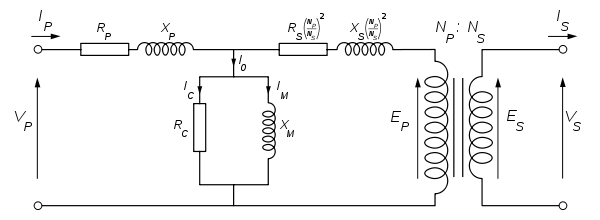
\includegraphics[width=0.7\textwidth]{fe14.png}}
	\caption{ejemplo de un Transformador en el circuito}
	\label{fe14}
\end{figure}

Hay tres tipos:

\begin{align*}
	 & \text{Núcleo de aire }                                     &  & \text{Núcleo de hierro }                  &  & \text{Núcleo variable} \\
	 & \begin{circuitikz}
		   \draw (0,0) node[ground](GND){} to [sV] ++(0,2) -- ++(1,0)
		   node[transformer, circuitikz/inductors/coils=6,
			   anchor=A1](T){};
		   \draw (T.A2) to[short, -*] (T.A2-|GND);
		   \draw (T-L2.midtap) to[short, *-o] (T.B1 |- T-L2.midtap);
		   \node [ocirc] at (T.B1){}; \node [ocirc] at (T.B2){};
	   \end{circuitikz} &  & \begin{circuitikz}
		                         \ctikzset{transformer L1/.style={inductors/width=1.8,
					                         inductors/coils=13}}
		                         % too small!
		                         \draw (0,0) node[transformer core](T1){};
	                         \end{circuitikz} &  & \begin{circuitikz}
		                                               \ctikzset{transformer L1/.style={inductors/width=1.8,
					                                               inductors/coils=13}}
		                                               % too small!
		                                               \draw (0,0) node[transformer core](T1){};
	                                               \end{circuitikz}
\end{align*}

Las fuentes de energía primaria, renovables y no renovables,
se aprovechan para producir energía
eléctrica en centrales que suelen
tener una estructura común, compuesta por calderas, turbinas generadores y refirgeradores.
Por lo tanto \textbf{la energía}

\smartdiagram[priority descriptive diagram]{
	Presenta incovenientes,
	Es la demandada del mundo,
	Dependemos de ella de muchas cosas,
	Se produce a partir de fuentes de energía,
	No se puede almacenar}


Cómo son las centrales de producción de energía eléctrica.
La térmica, nuclerar hidroeléctrica, geotérmica, solar térmica,
solar térmica, solar fotovoltaica, eólica y
maremotriz.


\section{Motores eléctricos}

\begin{equation}
	VI=Q+\tau\omega
\end{equation}

\begin{equation}
	VI\backsimeq I^2R+\tau\omega
\end{equation}

donde $tau$ es el toque, $\omega$ la velocidad angular y $Q$ el calor de salida


\subsection{Motor CD}

Un motor de corriente directa es un dispositivo simple de dos conductores, controlado eléctricamente que viene con un eje giratorio en el que se pueden montar ruedas, engranajes, hélices, etc\dots

La mayoría de los motores de corriente directa proporcionan velocidades de rotación entre 30000 y 8000 rpm a una tensión de un funcionamiento
normalmente entre 1.5 y 24V.

La tensión real aplicada a un motor puede ser ligeramente inferior para que el motor sea más lento o puede ser elevada para que el motor sea más rápido.

Cuando la tensión aplicada cae por debajo del 50\% de la tensión de funcionamiento especificada, el motor suele dejar de girar. Por el contrario, si la tensión aplicada supera la tensión de funcionamiento en un 30 \%, existe la posibilidad de que el motor se sobrecaliente y se dañe.

\begin{center}
	\begin{circuitikz}
		\draw (2,0) node[elmech](motor){M};
		\draw (motor.north) |-(0,2) to [R] ++(0,-2) to[
				dcvsource]++(0,-2) -| (motor.bottom);
		\draw[thick,->>](motor.right)--++(1,0)node[midway,
			above]{$\omega$};
	\end{circuitikz}
\end{center}

\subsubsection{Relevador}
El relé es un dispositivo electromagnético que funciona como un interruptor, el cual es controlado por un circuito
eléctrico compuesto de una bobina. Al inducir corriente sobre la bobina se genera un electroimán, con el cual se acciona
un juego de uno o varios contactos que permiten abrir o cerrar otros circuitos eléctricos independientes.

\begin{center}
	\begin{circuitikz}
		\draw
		(0,0) to[C] (1,0) to[toggle switch , n=Sw] (2.5,0)
		-- (2.5,-1) to[battery1] (1.5,-1) to[R] (0,-1) -| (0,0)
		(Sw.out 2) -| (2.5, 1) to[R] (0,1) -- (0,0);
	\end{circuitikz}
\end{center}

\begin{figure}[h!]
	\centering
	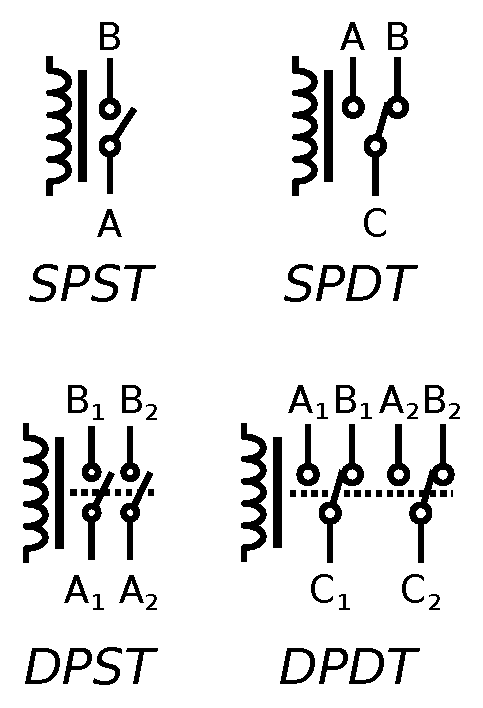
\includegraphics{fe15.pdf}
	\caption{Relevador}
\end{figure}

\subsubsection{Control direccional de los motores de CD}

Otro circuito muy popular utilizado para controlar la dirección de un motor (véase la figura \ref{fe15}), así como la velocidad es el puente $H$.

\begin{figure}[h!]
	\centerline{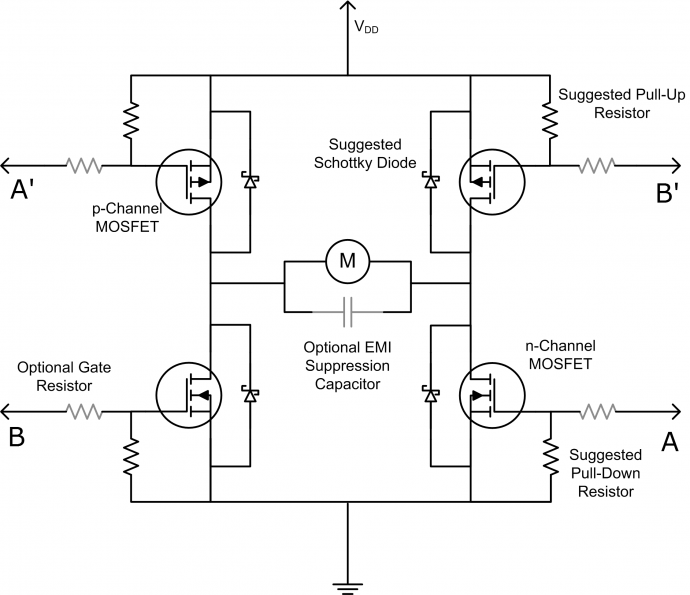
\includegraphics[width=0.3\textwidth]{fe15.png}}
	\caption{Puente mosfet h}
	\label{fe15}
\end{figure}

\begin{tikzpicture}[american]
	\draw (0,3) to [V=$v$](0,0);
	\draw (0,3) to (2,3);
	\draw (2,4) to (4,4);
	\draw (4,4) to (4,2);
	\draw (2,2) to (4,2);
	\draw (2,2) to (2,4);
	\draw (4,3) to (5,3) to (6,3) to (6,0);
	\draw (0,0) to (5,0) to (6,0);
\end{tikzpicture}


\subsection{Relevadores}

Es un interruptor eléctrico que permite el paso de la corriente eléctrica cuando está cerrado e interrumpirla cuando está abierto, pero que es accionado eléctricamente, no manualmente.

El relé está compuesto de una bobina conectada a una corriente. Cuando la bobina se activa produce un campo electromagnético que hace que el contacto del relé que está normalmente abierto se cierre y permita el paso de la corriente por un circuito para, por ejemplo, encender una lámpara o arrancar un motor. Cuando dejamos de suministrar corriente a la bobina, el campo electromagnético desaparece y el contacto del relé se vuelve a abrir, dejando sin corriente el circuito eléctrico que iba a esa lámpara o motor.

Los relés sirven para activar un circuito que tiene un consumo considerable de electricidad mediante un circuito de pequeña potencia -de 12 o 24 voltios- que imanta la bobina. Supongamos que queremos motorizar una puerta de un garaje o de la entrada de una finca. Para ello necesitaremos un mando a distancia que consigue activar a través de un receptor esa pequeña carga de potencia que pone en marcha el funcionamiento del relé: la bobina se imantará y cerrará el circuito eléctrico que alimenta el motor que sirve para abrir la puerta. También lo podremos utilizar para encender máquinas y motores, sistemas de alumbrado, etc.

En ocasiones, nos encontramos con circuitos de alumbrado que necesitan una gran potencia para su funcionamiento. Al activarlos y desactivarlos indirectamente, mediante el empleo de relés que funcionan con poca potencia, prevenimos posibles riesgos y accidentes.

%\begin{figure}[h!]
%	\centerline{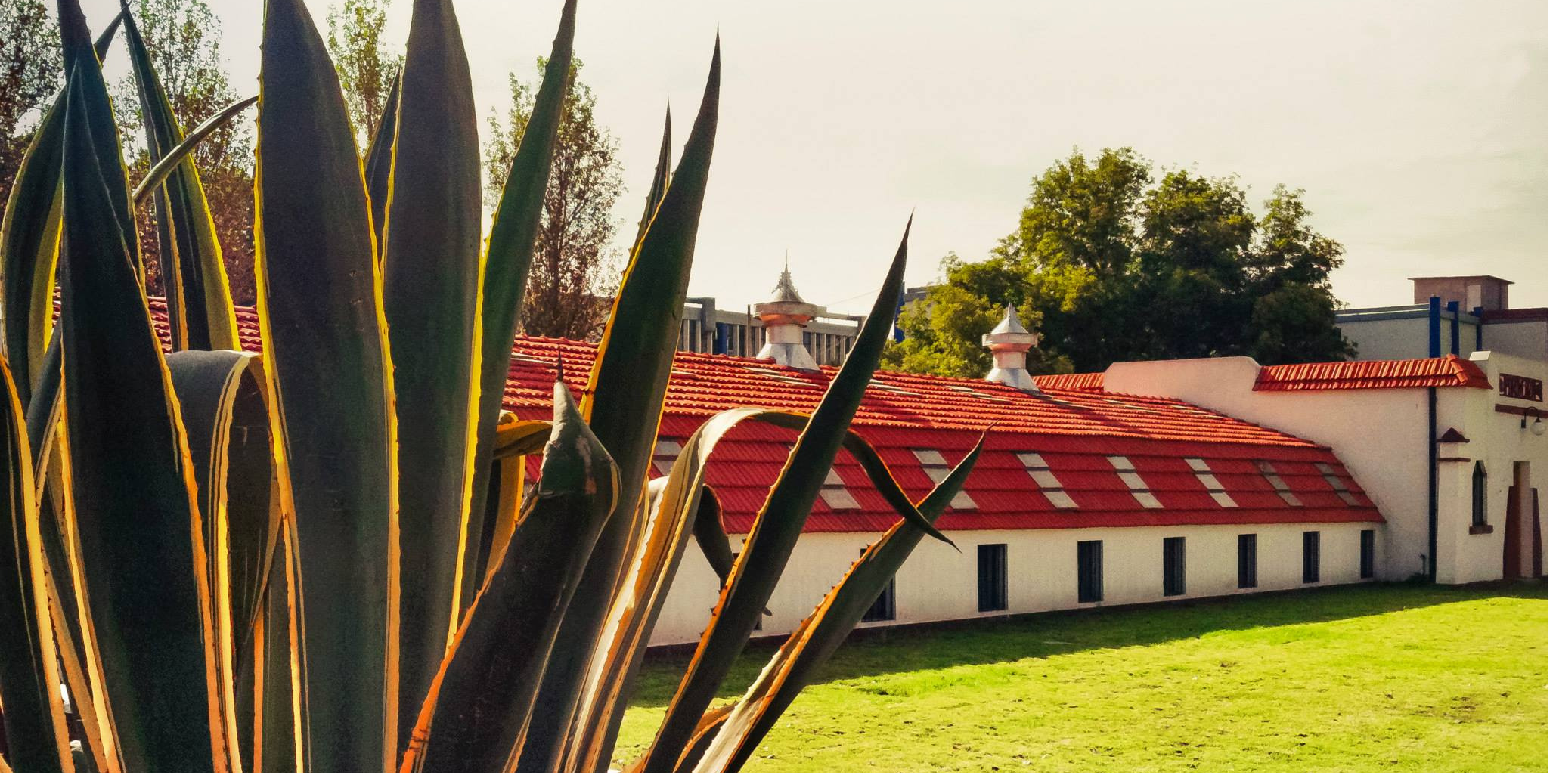
\includegraphics[width=0.7\textwidth]{1.jpg}}
%	\caption{Relevador}
%	\label{1}
%\end{figure}


\subsection{Motor Monofásico}

En los motores monofásicos (a diferencia de los trifásicos) el estator produce un campo magnético estacionario pulsante  que no es capaz por sí mismo de provocar un par de arranque Para generar ese par de arranque  el motor necesita de un devanado auxiliar desfasado $90^{\circ}$ respecto del devanado principal.

Esta característica se debe a que existe la necesidad de crear un campo bifásico partiendo de uno monofásico. Las diferentes disposiciones de estos devanados dictaminan la tipología del motor monofásico.

Pese a que pueden existir muchos tipos de motores monofásicos, habitualmente se les divide en dos grandes categorías. Son las siguientes: motor monofásico de fase partida, y de espira en cortocircuito o de sombra.

%\begin{figure}[h!]
%	\centerline{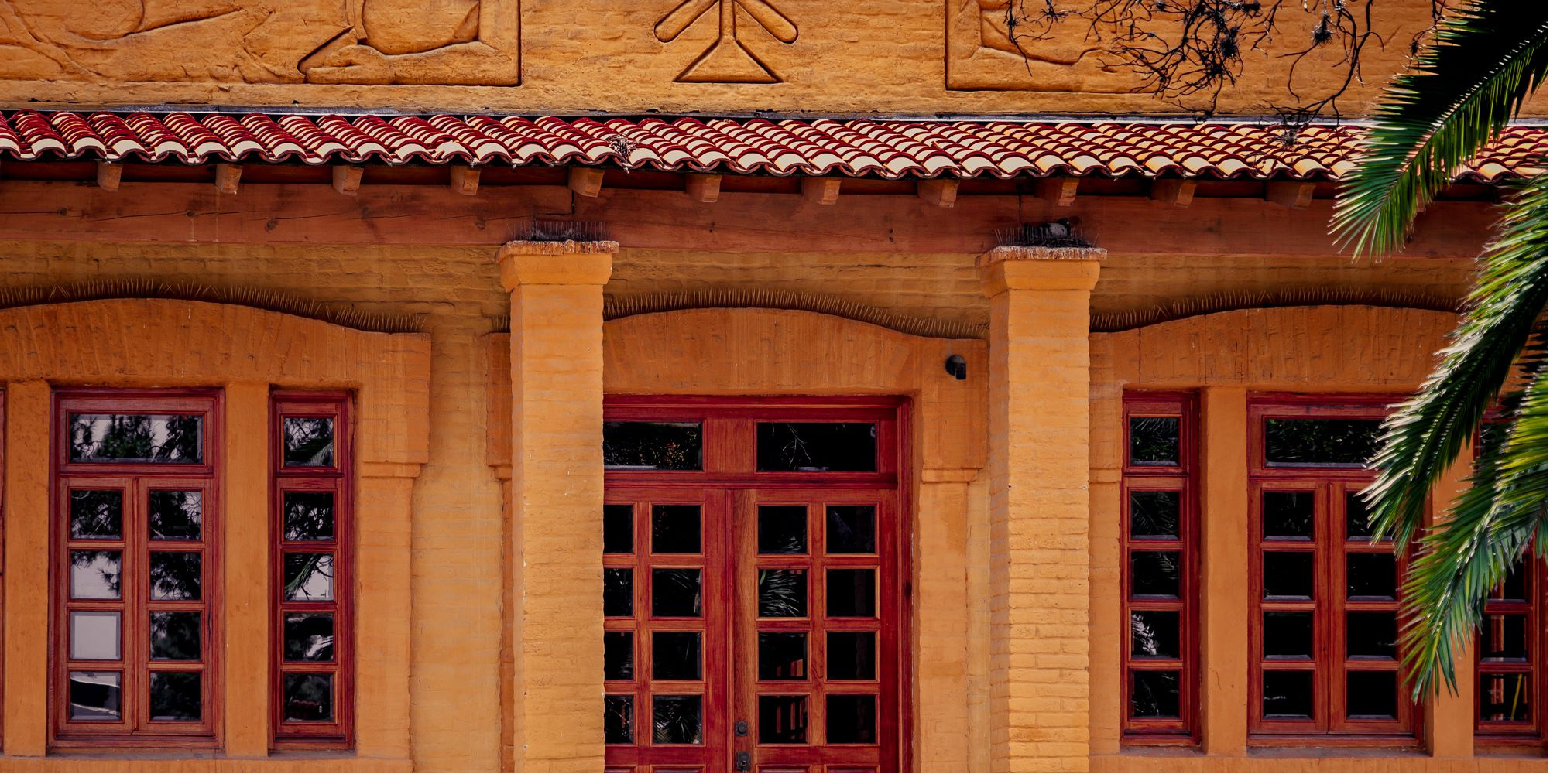
\includegraphics[width=0.7\textwidth]{2.jpg}}
%	\caption{Relevador}
%	\label{2}
%\end{figure}

\subsection{Bobina}

Un inductor, bobina o reactor es un componente pasivo de un circuito eléctrico que, debido al fenómeno de la autoinducción, almacena energía en forma de campo magnético.

\subsection{Capacitor}

Es un elemento pasivo diseñado para almacenar energía en us campo eléctrico. Los condensadires se utilizan ampliamente en la electrónica, las comunicaciones, las computadoras y los sistemas de energía.
Consiste en dos placas conductoras separadas por un aislante (o dieléctrico).

\textbf{Capacitor}
\begin{center}
	\begin{align*}
		 & Q=CV                         &
		 & \frac{dq}{dt}=C\frac{dv}{dt} &
		\frac{dq}{dt}=i=C\frac{dv}{dt}
	\end{align*}
	\begin{circuitikz}[american]
		\draw (0,0) to [capacitor] (3,0);
	\end{circuitikz}
\end{center}

\subsection{Estator}

El estátor es la parte fija de una máquina rotativa y uno de los dos elementos fundamentales para la transmisión de potencia (en el caso de motores eléctricos) o corriente eléctrica (en el caso de los generadores eléctricos), siendo el otro su contraparte móvil, el rotor. El término aplica principalmente a la construcción de máquinas eléctricas y dependiendo de la configuración de la máquina.

\subsubsection{Motor monofásico de fase partida}

Un motor monofásico de fase partida o de fase dividida es un motor de inducción con dos bobinados en el estator, uno principal y otro auxiliar o de arranque.

El motor de fase partida es uno de los distintos sistemas ideados para el arranque de los motores asíncronos monofásicos. Se basa en cambiar, al menos durante el arranque, el motor monofásico por un bifásico (que puede arrancar solo). El motor dispone de dos devanados, el principal y el auxiliar; además, lleva incorporado un interruptor centrífugo cuya función es la de desconectar el devanado auxiliar después del arranque del motor. Además del motor de fase partida existen otros sistemas para arrancar motores monofásicos como es el caso de motores de arranque por condensador.

\subsubsection{Motor monofásico de fase partida con capacitor}

Son motores técnicamente mejores que los motores de fase partida. También disponen de dos devanados, uno auxiliar y otro principal. Sobre el devanado auxiliar se coloca un capacitor (condensador) en serie, que tiene como función el de aumentar el par de arranque, entre 2 y 4 veces el par normal. Como se sabe, el capacitor desfasa la fase afectada en $90^{\circ}$, lo cual quiere decir, que el campo magnético generado por el devanado auxiliar se adelanta $90^{\circ}$ respecto al campo magnético generado por el devanado principal. Gracias a esto, el factor de potencia en el momento del arranque, está proximo al 100\%, pues la reactancia capacitiva del condensador $(X_C)$ anula la reactancia inductiva del bobinado $(x_L)$. Por lo demás, se consideran igual que los motores de fase partida, en cuanto a cambio de giro, etc. Lo único importante que debemos saber, es que con un capacitor en serie se mejora el arranque.

\subsection{Motores trifásicos}

El término a que se alimenta de energía eléctrica trifásica. Las instalaciones monofásicas son más propias de hogares, con tensiones que van de 120 a 230 voltios y potencias que quedan por debajo de los 10 Kw.

El motor trifásico está muy extendido en los usos destinados a instalaciones industriales o comerciales. Esto se debe, por un lado, a que suelen ser más pequeños y manejables que motores monofásicos de la misma potencia.

La potencia del motor trifásico varía en función de su uso y se fabrican en un rango muy grande de potencias, medidas en kilovatios o caballos de vapor. Generalmente están destinados al accionamiento de máquinas como bombas, montacargas, ventiladores, grúas, elevadores, etcétera.

\subsection{Motores trifásicos 2}

\subsection{Estator}
El estator es la parte fija y opera como la base del motor. Esta parte está constituida por una carcasa en la que se fijan una corona de chapas de hierro al silicio o acero al silicio, en las que están presentes unas ranuras. En estas ranuras es dónde se presentan, al tratarse de un motor trifásico, encontramos tres bobinas y tres circuitos diferentes. En cada circuito hay tantas bobinas como polos tiene el motor.

\subsection{Rotor}
El rotor es la parte móvil que se sitúa en el interior del estator. En el eje se inserta un núcleo magnético ranurado de acero al silicio en cuyas ranuras se colocan unas barras de cobre o aluminio (que realizan la función de conductores) en una disposición que se conoce como “jaula de ardilla”. Esto se debe a que las barras están unidas en cortocircuito por dos anillos, en la parte superior e inferior, confiriéndole una forma de jaula.

\subsection{Inversores}
Es un dispositivo que cambia o transforma una tensión de entrada de corriente continua a una tensión simétrica de salida (senoidal, cuadrada o triangular) de corriente alterna, con la magnitud y frecuencia deseada por el usuario o el diseñador.

Los inversores se utilizan en una gran variedad de aplicaciones, desde pequeñas fuentes de alimentación para computadoras, hasta aplicaciones industriales para controlar alta potencia. Los inversores también se utilizan para convertir la corriente continua generada por los paneles solares fotovoltaicos, acumuladores o baterías, etc, en corriente alterna y de esta manera poder ser inyectados en la red eléctrica o usados en instalaciones eléctricas aisladas.

El aire acondicionado inversor, es un tipo de acondicionador de aire que utiliza un inversor de potencia para fijar la velocidad del motor del compresor y así dejar constante la temperatura, con lo que se ahorra un mínimo del 40\% de la electricidad.

\subsection{Aplicación de los motores}

\section{Anexo de problemas}


\begin{enumerate}
	%%%%%%%%%%%%%%%%%%%%%%%%%%%%%%%%%%%%% PROBLEMA 1 %%%%%%%%%%%%%%%%%%%%%%%%%%%%%%%%%%%
	\item Encuentre $R_{ab}$

	      \begin{center}
		      \begin{circuitikz}[american]
			      \draw (0,0) to [open, l=$b$, *-](0,0.9);
			      \draw (0,2.9) to [open, l=$a$, -*](0,3);
			      \draw (0,0) to [open, l=$R_{ab}$](0,3) to [R=$16\Omega$](3,3) to [R=$18\Omega$](0,0) to (3,0) to [R=$9\Omega$](3,3) to [R=$20\Omega$](6,0) to [R=$2\Omega$](3,0);
			      \draw (3,3) to [R=$5\Omega$](6,3) to [R=$1\Omega$](6,0);
			      \draw (3,3) to (3,5) to [R=$20\Omega$](6,5) to (6,3);
		      \end{circuitikz}
	      \end{center}

	      \textit{Sol. }

	      Se observa que $20\Omega$ estan en paralelo con $5\Omega$ en la parte superior del circuito, se le nombrará $R_1$.

	      \begin{equation}
		      \frac{1}{R_1}=\frac{1}{20\Omega}+\frac{1}{5\Omega}=\frac{1}{4}=4\Omega=R_1
	      \end{equation}

	      $R_1$ está en serie con $1\Omega$, se suman para obtener $R_2$

	      \begin{equation}
		      R_2= R_1+1\Omega= 4\Omega+ 1\Omega=5\Omega
	      \end{equation}

	      Se obtiene que $R_2$ está en paralelo con $20\Omega$:

	      \begin{equation}
		      \frac{1}{R_3}=\frac{1}{R_2}+\frac{1}{20\Omega}=\frac{1}{5\Omega}+\frac{1}{20\Omega}=\frac{1}{4}=4\Omega=R_3
	      \end{equation}

	      Al mismo tiempo $R_3$ está en serie con $2\Omega$, así que sumando nos da $R_4$

	      \begin{equation}
		      R_4=4\Omega+2\Omega=6\Omega
	      \end{equation}

	      Se suman las resistencias $18\Omega$ y $9\Omega$ en paralelo antes de adicionarlo con la $R_4$

	      \begin{equation}
		      \frac{1}{18}\Omega+\frac{1}{9}\Omega=\frac{1}{6}\Omega=6\Omega=R_5
	      \end{equation}

	      Procedemos a sumar en paralelo $R_4$ y $R_5$:

	      \begin{equation*}
		      \frac{1}{6}\Omega+\frac{1}{6}\Omega=3\Omega=R_6
	      \end{equation*}

	      Y se concluye sumando $R_6$ con $16\Omega$:

	      \begin{equation*}
		      R_{ab}= 3\Omega+16\Omega=19\Omega
	      \end{equation*}

	      %%%%%%%%%%%%%%%%%%%%%%%%%%%%%%%%%%%%% PROBLEMA 2 %%%%%%%%%%%%%%%%%%%%%%%%%%%%%%%%%%%

	\item Determine la resistencia equivalente entre los puntos $a$ y $b$ para la combinación que se muestra en la siguiente figura. Sí Una corriente de 5.0 $A$ fluye en el circuito desde el punto a y hasta el punto $b$. ¿Cuál es la diferencia de potencial de $a$ a $b$? ¿Cuánta corriente fluye por el resistor de 12.0$\Omega$ ?



	      \begin{center}
		      \begin{circuitikz}[american]
			      \draw (0,0) to [R=$9\Omega$](3,0) to (3,3) to [R=$3\Omega$](7,3) to [R=$2\Omega$](6,0) to [R=$6\Omega$](3,0);
			      \draw (0,0) to [short, l_=$a$](0,0.3);
			      \draw (3,0) to [short, l=$c$](3,0.3);
			      \draw (6,0) to [short, l=$d$](6,0.3);
			      \draw (7,-3) to [short, l=$b$](7,-3.1);
			      \draw (3,0) to (3,-3) to [R=$5\Omega$](6,-3) to [R=$12\Omega$](3,0);
			      \draw (7,-3) to (6,-3) to [R=$7\Omega$](6,0);
		      \end{circuitikz}
	      \end{center}


	      \textit{Sol. }

	      Para calcular $R_{ab}$, para ello, se empieza con $3\Omega$ y $2\Omega$ en serie:

	      \begin{equation*}
		      3\Omega+2\Omega=5\Omega=R_1
	      \end{equation*}

	      Seguido de sumar en paralelo con $6\Omega$:

	      \begin{equation*}
		      5\Omega+6\Omega=\frac{30}{11}\Omega=\frac{11}{30}=R_2
	      \end{equation*}

	      Se suma en serie con $7\Omega$

	      \begin{equation*}
		      \frac{30}{11}\Omega+\frac{1}{7}\Omega=\frac{107}{11}=R_3
	      \end{equation*}

	      Así mismo se suma en paralelo con $12\Omega$:

	      \begin{equation*}
		      \frac{11}{107}+\frac{1}{12}=\frac{239}{1284}\Omega=\frac{1284}{239}\Omega=R_4
	      \end{equation*}

	      Ahora se procede a sumarse en serie con $9\Omega$

	      \begin{equation*}
		      \frac{1284\Omega}{239}\Omega+9\Omega=\frac{6420}{2479}\Omega=\frac{6420}{2479}\Omega=11.58\Omega
	      \end{equation*}

	      Para obtener la diferencia de potencial total entre $a$ y $b$ utilizamos la ley de ohm $V=IR$:

	      \begin{equation*}
		      V=(5A)(11.58)\approx 58V
	      \end{equation*}

	      Lo que implica que el volaje entre $a$ y $c$ es corriente por resistencia: $5A\cdot 9\Omega=45V$ Por lo tanto el voltaje entre $c$ y $b$ será voltaje total - voltaje $ac$:

	      \begin{equation}
		      V_{cb}=V_T-V_{ac}
	      \end{equation}

	      Eso es igual a $58V-45V=13V$, como entre las terminales $a$ y $c$ hay cuatro conexiones distintas en paralelo, el voltaje siguie siendo $13V$ para cada una de las diferentes ramas, pero con su respectiva corrietne determinada por $I=\frac{V}{R}$.

	      Procedemos a resolver la $I_1$:

	      \begin{equation*}
		      I_1=\frac{13V}{3\Omega+2\Omega}=2.6A
	      \end{equation*}

	      Para $I_2$ se tiene el mismo voltaje pues están en paralelo, sobre el valor de la resistencia de $6\Omega$

	      \begin{equation*}
		      I_2=\frac{13V}{6\Omega}=2.16A
	      \end{equation*}

	      Para $I_3$:

	      \begin{equation*}
		      I_3=\frac{13V}{12\Omega}=1.083A
	      \end{equation*}

	      Homólogamente:

	      \begin{equation*}
		      I_4=\frac{13V}{5\Omega}=2.6\Omega
	      \end{equation*}

	      $I_5$ será la suma de $I_1+I_2$ de acuerdo de la primera le de Kirchhoff, que encuncia que la suma de la corriente que entra en nodo, es igual a la suma de las corrientes que salen.

	      \begin{equation*}
		      I_5=I_1+I_2=2.6A+2.16A=4.76
	      \end{equation*}

	      %%%%%%%%%%%%%%%%%%%%%%%%%%%%%%%%%%%%% PROBLEMA 3 %%%%%%%%%%%%%%%%%%%%%%%%%%%%%%%%%%%
	\item Las corrientes en el circuito de la siguiente figura son estacionarias. Determine $I_1$, $I_2$, $I_3$ y la carga en el capacitor.


	      \begin{center}
		      \begin{circuitikz}[american]
			      \draw (0,0) to (0,3) to [I=$I_3$](3,3)to [R=$5\Omega$](6,3) to (6,0);
			      \draw  (0,0) to [capacitor=$C{=}2\mu F$](2,0) to [R=$3\Omega$, i=$I_2$](4,0) to [battery1=$6V$](6,0);
			      \draw (6,0) to (6,-3) to  [R=$7\Omega$](3,-3);
			      \draw (0,-3) to [battery1=$15V$](3,-3);
			      \draw (0,-3) to [I=$I_1$](0,0);
		      \end{circuitikz}
	      \end{center}

	      \textit{Sol. }
	      Dado que el capacitor está conectado en serie por donde pasa la corriente $I_2$, y ha estado conectado a la fuente de voltaje, este capacitor (cargado) se comporta como un circuito abierto, por lo que $I_2=0$ y sólo queda analizar el resto del circuito, para el cual, evidentemente $I_1=I_3$
	      Por lo que se tiene:
	      \begin{equation*}
		      I_1=\dfrac{V}{R_T} = \dfrac{15V}{12\Omega}=1.25 A =I_3
	      \end{equation*}

	      %%%%%%%%%%%%%%%%%%%%%%%%%%%%%%%%%%%%% PROBLEMA 4 %%%%%%%%%%%%%%%%%%%%%%%%%%%%%%%%%%%

	\item Obtener la resistencia equivalente y usarla para calcular la corriente $i$. (Utilizar transformaciones $\delta$ y $Y$, para simplificar el circuito).


	      \begin{center}
		      \begin{circuitikz}[american]
			      \draw (1,6) to [V=$120V$](1,0);
			      \draw (1,6) to [short, i=$i$, l_=$a$](3,6) to [short, l_=$a$, *-](8,6) to [R=$30\Omega$](8,0) to (1,0);
			      \draw (3,0) to [R=$15\Omega$](3,3) to [R=$12.5\Omega$](3,6);
			      \draw (6,0) to [R=$20\Omega$](6,3) to [R=$10\Omega$, -*](6,6);
			      \draw (3,3) to [R=$5\Omega$](6,3);
		      \end{circuitikz}
	      \end{center}

	      \textit{Sol. }

	      Si se convierte la red en forma de $y$, se asignan como $R_1=10\Omega$, $R_2=20\Omega$ y $R_3=5\Omega$

	      Se aplica la conversión de estrella a delta, como se muestra en el cirucito inferior:

	      \begin{center}
		      \begin{circuitikz}[american]
			      \draw (0,5) to [R=$R_b$](3,0) to [R=$R_3$](3,3) to [R=$R_2$](6,5) to [R=$R_a$](3,0);
			      \draw (3,3) to [R=$R_1$](0,5) to [R=$R_c$](6,5);
		      \end{circuitikz}
	      \end{center}

	      \begin{align}
		       & R_b=\frac{R_1\cdot R_2+R_2\cdot R_3+R_3\cdot R_1}{R_2}=\frac{350\Omega}{20\Omega}=17.5\Omega \\
		       & R_c=\frac{R_1\cdot R_2+R_2\cdot R_3+R_3\cdot R_1}{R_3}=\frac{350\Omega}{5\Omega}=70\Omega
	      \end{align}

	      Ahora se obtiene $R_a$:

	      \begin{equation}
		      R_a=\frac{R_1\cdot R_2+R_2\cdot R_3+R_3\cdot R_1}{R_1}=\frac{350\Omega}{10\Omega}=35\Omega
	      \end{equation}

	      Obtenemos el siguiente circuito:

	      \begin{center}
		      \begin{circuitikz}[american]
			      \draw (1,6) to [short, open](1,0);
			      \draw (1,6) to [short, i=$i$](3,6) to (8,6) to [R=$30\Omega$](8,0) to (1,0);
			      \draw (3,0) to [R=$15\Omega$](3,3) to [R=$12.5\Omega$](3,6);
			      \draw (6,0) to [R=$70\Omega$](6,6);
			      \draw (6,6) to [R=$17.5\Omega$](3,3);
			      \draw (6,0) to [R=$35\Omega$](3,3);
			      \draw (1,6) to [short, l_=$a$, *-](1,5.9);
			      \draw (1,0) to [short, l=$b$, *-](1,0.1);
		      \end{circuitikz}
	      \end{center}

	      Se combinan en paralelo las resistencias del extremo derecho:

	      \begin{equation}
		      \frac{1}{R_1}=\frac{1}{30\Omega}+\frac{1}{70\Omega}=\frac{1}{21}\Omega=21\Omega=R_1
	      \end{equation}

	      Así mismo, en la sección izquierda, se combinan en paralelo:

	      \begin{equation}
		      R_2=12.5\Omega\mid \mid 17.5\Omega=\frac{12.5\Omega \times 30\Omega}{70\Omega+30\Omega}=7.292\Omega=R_2
	      \end{equation}

	      Se resuelve en paralelo $15\Omega$ y $35\Omega$

	      \begin{equation}
		      R_3=15\Omega\mid \mid 35\Omega=\frac{15\Omega \times 35\Omega}{15\Omega+35\Omega}=10.5\Omega=R_3
	      \end{equation}

	      Se concluye la resistencia equivalente con tres resistencias sobrantes, los cuales son:

	      \begin{equation}
		      R_{ab}=(7.292\Omega+10.5\Omega)\mid \mid 21=\frac{17.792\times 21}{17.792+21}=9.632\Omega
	      \end{equation}

	      Finalmente se obtiene la corriente:

	      \begin{equation}
		      i=\frac{v_s}{R_{ab}}=\frac{120V}{9.632\Omega}=12.458A
	      \end{equation}

	      %%%%%%%%%%%%%%%%%%%%%%%%%%%%%%%%%%%%% PROBLEMA 5 %%%%%%%%%%%%%%%%%%%%%%%%%%%%%%%%%%%

	\item Para el siguiente circuito encontrar:
	      \begin{enumerate}
		      \item $v_1$ y $v_2$,
		      \item la potencia disipada en la resistencia de $3k\Omega$  y $20k\Omega$
		      \item La potencia suministrada por la fuente de corriente.
	      \end{enumerate}

	      \begin{center}
		      \begin{tikzpicture}[american]
			      \draw (0,3) to [R=$R_1{=}3k\Omega$, v=$v_1$](0,0);
			      \draw (2.5,0) to [I=$I_i{=}30mA$](2.5,3);
			      \draw (0,3) to [R=$R_4{=}1k\Omega$](2,3);
			      \draw (2,3) to (4,3) to[R=$R_3{=}5K\Omega$] (4,0);
			      \draw(4,3) to (7,3) to [R=$R_2{=}20K\Omega$, v=$v_2$](7,0) to (0,0);
		      \end{tikzpicture}
	      \end{center}
	      \textit{ Sol. }

	      Como primer paso empleamos la transformación de fuentes utilizando la corriente $I_i=3mA$ y las resistencias en serie $R_1=1k\Omega$ con $R_4=3k\Omega$.  \\
	      Por lo que tenemos $V_i=(30mA)(R_1=1k\Omega+R_4=3k\Omega)= (30\times10^{-3}A)((3+1)10^3\Omega)=(30\times10^{-3}A)(4\times10^3$)= $120V=V_i$. Quedándo entonces el siguiente circuito:
	      \begin{center}
		      \begin{tikzpicture}[american]
			      \draw (0,3) to [V=$V_i{=}120V$](0,0);
			      \draw (0,3) to [short, l=$a$](0,3.1);
			      \draw (4,3) to [short, l_=$b$](4,3.1);
			      \draw (4,0) to [short, l=$c$](4,0.1);
			      \draw (0,3) to [R=$R_4{=}1k\Omega$](2,3);
			      \draw (2,3) to [R=$R_1{=}3k\Omega$](4,3) to[R=$R_3{=}5\Omega$] (4,0);
			      \draw(4,3) to (7,3) to [R=$R_2{=}20\Omega$, v=$v_2$](7,0) to (0,0);
		      \end{tikzpicture}
	      \end{center}

	      El siguiente paso es calcular la resistencia equivalente entre $R_3$ y $R_2$  que están conectadas en paralelo.

	      \begin{equation*}
		      R_{23}= \frac{5k\Omega \times 20k\Omega}{5k\Omega+20k\Omega}=4k\Omega
	      \end{equation*}

	      Calculamos la resistencia equivalente sumando $R_1+R_4+R_{23}$

	      \begin{equation*}
		      R_T=3k\Omega+1k\Omega+4k\Omega=8k\Omega
	      \end{equation*}

	      Se procede a calcular la intesidad total:

	      \begin{equation*}
		      I_T=\frac{V}{R}=\frac{12V}{8k\Omega}=15mA
	      \end{equation*}

	      El voltaje de $a$ a $b$ está determinado por la fórmula $V=IR$:

	      \begin{equation*}
		      V_{ab}=15mA\times 4k\Omega=60V
	      \end{equation*}

	      Eso implica de $b$ a $c$ tendremos un voltaje determinado por:

	      \begin{equation*}
		      V_{bc}=V_T-V_{ab}=120V-60V=60V
	      \end{equation*}

	      Será el mismo para $V_2$ porque están conectados en paralelo.

	      Para $V_1$

	      \begin{equation*}
		      V_1=I_T\times R_1=15mA\times 3k\Omega=45V
	      \end{equation*}

	      Ahora se procede a operar la potencia dicipada para $R_1$:

	      \begin{equation*}
		      P_1=V_1I_T=45V\cdot 15mA=675mW
	      \end{equation*}

	      a potencia en la resistencia dos es igual a :

	      \begin{equation*}
		      P_2=V_2I_{bc}=60V\cdot 15mA=900mW
	      \end{equation*}

	      Para el inciso C, ya se cuenta con el voltaje que es de $60V$, y la inntensidad de corriente suministrada de $30mA$:

	      \begin{equation*}
		      P_F= V_1I_i=60V\cdot 30mA=1.8 W
	      \end{equation*}

	      %%%%%%%%%%%%%%%%%%%%%%%%%%%%%%%%%%%%% PROBLEMA 6 %%%%%%%%%%%%%%%%%%%%%%%%%%%%%%%%%%%

	\item Encontrar la resistencia equivalente y la corriente en el siguiente circuito.


	      \begin{center}
		      \begin{circuitikz}[american]
			      \draw (0,9) to [V=$20V$](0,0);
			      \draw (0,9) to [R=$4\Omega$,i=$I$](3,9) to [R=$2\Omega$](5,9) to [R=$1\Omega$](5,6) to [R=$12\Omega$](3,6) to [R=$8\Omega$](3,3) to [R=$4\Omega$](5,3) to [R=$3\Omega$](5,0) to [R=$5\Omega$](3,0) to [R=$10\Omega$](3,3);
			      \draw (3,3.2) to [short, l_=$a$](3,3.2);
			      \draw (5,3) to [short, l_=$b$](5,3.1);
			      \draw (3,0.2) to [short, l_=$c$](3,0.2);
			      \draw (3,6.2) to [short, l_=$d$](3,6.2);
			      \draw (5,6) to [short, l_=$e$](5,6.1);
			      \draw (5,3) to [R=$2\Omega$](5,6);
			      \draw (3,6) to [R=$6\Omega$](3,9);
			      \draw (0,0) to (3,0);
		      \end{circuitikz}
	      \end{center}


	      \textit{Sol. }
	      Primero sumamos en serie las resistencias de la esquina superior e inferior derecha, quedando el siguiente esquema:

	      \begin{center}
		      \begin{circuitikz}[american]
			      \draw (0,9) to [V=$20V$](0,0);
			      \draw (0,9) to [R=$4\Omega$,i=$I$](3,9) to (5,9) to [R=$3\Omega$](5,6) to [R=$12\Omega$](3,6) to [R=$8\Omega$](3,3) to [R=$4\Omega$](5,3) to [R=$8\Omega$](5,0) to (3,0) to [R=$10\Omega$](3,3);
			      \draw (5,3) to [R=$2\Omega$](5,6);
			      \draw (3,6) to [R=$6\Omega$](3,9);
			      \draw (3,3.2) to [short, l_=$a$](3,3.2);
			      \draw (5,3) to [short, l_=$b$](5,3.1);
			      \draw (3,0) to [short, l_=$c$](3,0.1);
			      \draw (3,6.2) to [short, l_=$d$](3,6.3);
			      \draw (5,6) to [short, l_=$e$](5,6.1);
			      \draw (3,9.2) to [short, l_=$f$](3,9.2);
			      \draw (0,0) to (3,0);
		      \end{circuitikz}
	      \end{center}

	      Y continuamos el desarrollo del ejerciocio empleando transformación delta-estrella, para esto procedemos a utilizar a las tres resistencias de la esquina inferior derecha aislándolas quedando así:

	      \begin{center}
		      \begin{circuitikz}[american]
			      \draw (0,5) to [R=$10\Omega$](3,0) to [R=$R_3$](3,3) to [R=$R_2$](6,5) to [R=$8\Omega$](3,0);
			      \draw (3,3) to [R=$R_1$](0,5) to [R=$4\Omega$](6,5);
			      \draw (0,5.2) to [short, l_=$a$](0,5.4);
			      \draw (6,5) to [short, l_=$b$](6,5.2);
			      \draw (3,0) to [short, l_=$c$](3,0.2);
		      \end{circuitikz}
	      \end{center}

	      Teniendo como base este esquema encontraremos $R_1, R_2$ y $R_3$ como sigue:


	      \begin{align*}
		      R_1= \frac{4\Omega \times 10\Omega}{4\Omega +10\Omega +8\Omega} = \frac{40\Omega}{22}=\frac{20}{11}\Omega
		      \\&\\
		      R_2= \frac{4\Omega \times 8\Omega}{4\Omega +10\Omega +8\Omega} = \frac{32\Omega}{22}=\frac{16}{11}\Omega
		      \\&\\
		      R_3= \frac{10\Omega \times 8\Omega}{4\Omega +10\Omega +8\Omega} = \frac{80\Omega}{22}=\frac{40}{11}\Omega
	      \end{align*}
	      Y se realiza un prcedimiento similar para las tres resistencias de la esquina superior derecha:

	      \begin{center}
		      \begin{circuitikz}[american]
			      \draw (0,0) to [R=$12\Omega$](6,0);
			      \draw (6,0) to [R=$3\Omega$](3,6);
			      \draw (0,0) to [R=$6\Omega$](3,6);
			      \draw (3,2.5) to [R=$R_6$](6,0);
			      \draw (0,0) to [R=$R_5$](3,2.5);
			      \draw (3,2.5) to [R=$R_4$](3,6);
			      \draw (-0.8,0) to [short, l_=$d$](-0.8,0.2);
			      \draw (6,0) to [short, l_=$e$](6,0.2);
			      \draw (3,6) to [short, l_=$f$](3,6);
		      \end{circuitikz}
	      \end{center}

	      Ahora calculamos $R_4,R_5$ y $R_6$:

	      \begin{align*}
		      R_4= \frac{6\Omega \times 3\Omega}{6\Omega +3\Omega +12\Omega} = \frac{18\Omega}{21}=\frac{6}{7}\Omega
		      \\&\\
		      R_5= \frac{6\Omega \times 12\Omega}{6\Omega +3\Omega +12\Omega} = \frac{72\Omega}{21}=\frac{24}{7}\Omega
		      \\&\\
		      R_6= \frac{3\Omega \times 12\Omega}{6\Omega +3\Omega +12\Omega} = \frac{36\Omega}{21}=\frac{12}{7}\Omega
	      \end{align*}

	      Por lo que sustituyendo los valores de las resistencias encontradas $R_1, R_2, R_3, R_4, R_5$ y $R_6$
	      se tiene el siguiente circuito:

	      \begin{center}
		      \begin{circuitikz}[american]
			      \draw (0,9) to [V=$20V$](0,0);
			      \draw (0,9) to [R=$4\Omega$,i=$I$](4,9);
			      \draw (3,6) to [R=$8\Omega$](3,3);
			      \draw (5,3) to [R=$2\Omega$](5,6);
			      \draw (0,0) to (3,0);
			      \draw (3,6) to [R=$R_5{=}\frac{24}{7}\Omega$](4,7.5);
			      \draw (4,7.5) to [R=$R_6{=}\frac{12}{7}\Omega$](5,6);
			      \draw (4,7.5) to [R=$R_4{=}\frac{6}{7}\Omega$](4,9);
			      \draw (4,1.5) to [R=$R_1{=}\frac{20}{11}$](3,3);
			      \draw (5,3) to [R=$R_2{=}\frac{16}{11}$] (4,1.5);
			      \draw (4,1.5) to [R=$R_3{=}\frac{40}{11}$] (4,0);
			      \draw (4,0) to (3,0);
		      \end{circuitikz}
	      \end{center}

	      Como se observa en el esquema, las resistencias $R_5$, la de $8\Omega$ y $R_1$ están conectadas en serie, las sumaremos de esta manera y al resultado lo llamaremos $R_{e_1}$, para el lado derecho se realia un procedimiento semejante y la resistencia será nomrada $R_{e_2}$, mismas que están conectadas en paralelo entre sí, por lo que se realiza el producto entre la suma y al final se suman en serie con la resistencia de $4\Omega$ obteniendo la resistencia equivalente total:

	      \begin{align*}
		      R_{e_1}= \frac{24}{7}+8+\frac{20}{11}=\frac{
		      1020}{77} \\&\\
		      R_{e_2}= \frac{12}{7}+2+\frac{16}{11}=\frac{
		      398}{77}  \\&\\
		      \implies R_{e_1}//R_{e_2} = \dfrac{\dfrac{
				      1020}{77}\cdot {\dfrac{
					      398}{77}}}{\dfrac{
				      1020}{77}+\dfrac{
				      398}{77}}= \dfrac{68.470231}{18.415584}=3.718059 \Omega
		      \\&\\
		      \implies R_T= R_7 + R_4 + R_{e_1e_2} + R_3=4+\frac{6}{7}+3.718+\frac{40}{11}=12.2115 \Omega
	      \end{align*}
	      Por lo que la corriente estará determinada por la ley de Ohm:
	      \begin{equation*}
		      I_T=\dfrac{V}{R_T}= \dfrac{20 V}{12.2115 \Omega}=1.6378 A
	      \end{equation*}


	      %%%%%%%%%%%%%%%%%%%%%%%%%%%%%%%%%%%%% PROBLEMA 7 %%%%%%%%%%%%%%%%%%%%%%%%%%%%%%%%%%%

	\item Para el siguiente circuito:
	      \begin{enumerate}
		      \item Encuentre las corrientes $I$ e $I_6$
		      \item Encuentre los voltajes $v_1$ y V5
		      \item Encuentre la potencia entregada al resistor de $6k \Omega$
	      \end{enumerate}


	      \begin{center}
		      \begin{tikzpicture}[american]
			      \draw (0,0) to [V=$e$, i=$I$](0,3) to (4,3);
			      \draw (3.5,3) to [R=$12K\Omega$](3.5,0);
			      \draw (2,2.5) to (5,2.5) to [R=$40\Omega$](5,0.5) to (2,0.5) to [R=$R_1{=}10\Omega$](2,2.5);
			      \draw (4,3) to (8,3) to (8,2) to [R=$R_6{=}10{.}4K\Omega$](8,0) to (0,0);
			      \draw (5.5,2) to (5.5,4) to [R=$R_4{=}9K\Omega$](8,4) to [I=$I_6$](8,2) to [R, l_=$R_5{=}6K\Omega$](5.5,2);
		      \end{tikzpicture}
	      \end{center}


	      \textit{Sol. }


	      \begin{enumerate}
		      \item Para encontrar el valor de $I$ e $I_6$, primero se calcula la resistencia total:

		            \begin{equation*}
			            R_a=\frac{1}{R_1}+\frac{1}{R_2}+\frac{1}{R_3}=\frac{1}{12k\Omega}+\frac{1}{12k\Omega}+\frac{1}{3k\Omega}=\frac{1}{2k\Omega}=2k\Omega
		            \end{equation*}

		            Homologamente:

		            \begin{equation*}
			            R_b=\frac{1}{R_4}+\frac{1}{R_5}=\frac{1}{9k\Omega}+\frac{1}{6k\Omega}=\frac{5}{18}k\Omega=3.6k\Omega
		            \end{equation*}

		            Se Suma primero $R_b$ y $R_6$ en serie:

		            \begin{equation*}
			            R_c=R_b+R_6=3.6k\Omega+10.4k\Omega=14k\Omega
		            \end{equation*}

		            Después sumamos $R_c$ y $R_a$ en paralelo para obtener $R_T$

		            \begin{align*}
			             & \frac{1}{R_T}=\frac{1}{R_c}+\frac{1}{R_a}=\frac{1}{14k\Omega}+\frac{1}{2k\Omega}=\frac{4}{7k\Omega} \\
			             & R_T=\frac{7}{4}k\Omega=1.75k\Omega                                                                  \\
			             & I=\frac{28V}{1.75k\Omega}=16\times 10^{-3}A
		            \end{align*}

		            Para $I_6$, tomando en cuenta las letes de Kirchhoff, se desarrolla un sistema de ecuaciones por divisor de corriente. en donde $I_6=I_2$ planteado en nuestro sistema de ecuaciones siguiente:

		            \begin{align*}
			             & I=I_1+I_2                            \\
			             & 28V-2k\Omega I_1=0                   \\
			             & 28V-10.4k\Omega I_2-3.6k\Omega I_2=0
		            \end{align*}

		            resolviendolo obtenemos que:

		            \begin{align}
			             & I_1=14\times 10^{-3}A \\
			             & I_6=2\times 10^{-3}A
		            \end{align}

		            Luego para resolver el valor del voltaje, se procede a sustituir las corrientes.

		            \begin{align}
			             & V_1=I_1\cdot R_1=\left(14\times 10^{-3}A\right)\left(12k\Omega\right)=168V \\
			             & V_5=I_6\cdot R_5=\left(2\times 10^{-3}A\right)\left(6k\Omega\right)=12V
		            \end{align}

		      \item Para la potencia entregada al resistor de $6k\Omega$:

		            \begin{equation*}
			            P=I_6^2\times R=\left(2\times 10^{-3}A\right)\left(6k\Omega\right)=12V
		            \end{equation*}

		      \item 2
	      \end{enumerate}



	      %%%%%%%%%%%%%%%%%%%%%%%%%%%%%%%%%%%%% PROBLEMA 8 %%%%%%%%%%%%%%%%%%%%%%%%%%%%%%%%%%%

	\item Cada una de las celdas que se muestran en la figura siguiente tiene una fuerza electromotriz (diferencia de potencial) de $1.50 V$ y una resistencia interna de $0.0750\Omega$. Encuentre $I_1$, $I_2$ e $I_3$.


	      \begin{center}
		      \begin{tikzpicture}[american]
			      \draw (0,3) to [I=$I_1$](0,0);
			      \draw (0,3) to (1,3);
			      \draw (1,4) to [battery1](2,4) to [R](3,4) to [battery1](4,4) to [R](5.5,4) to (5.5,2);
			      \draw (1,4) to  (1,2);
			      \draw (1,2) to [battery1](2,2) to [R](3,2) to [battery1](4,2) to [R](5.5,2);
			      \draw (5.5,3) to (6,3) to (6,0);
			      \draw (0,0) to [R=$3\Omega$](6,0);
		      \end{tikzpicture}
	      \end{center}

	      \textit{Sol. }


	      Como primer paso se simplificará el circuito para tener un solo valor de $V$ y una $R_{eq}$ para calcular la corriente ($I$) total y apartir de ahí las que pide el problema.\\

	      Las resistencias internas de las baterias se sumaran en serie resultando 2 resistencias en paralelo de $0{.}15 \Omega$ que tambien se sumaran, ahora en paralelo: resultando una resistencia de $0{.}075 \Omega$ que puede sumarse con la de $3 \Omega$, dejando la Resistencia eqivalente del circuito como $R_{eq}= 3{.}075 \Omega$. \\

	      Las baterias que estan en paralelo las podemos juntar, sumando sus fem´s, quedandonos 2 baterias en paralelo de $Fem=3 V$.\\

	      \begin{center}
		      \begin{tikzpicture}[american]
			      \draw (0,3) to [I=$I_1$](0,0);
			      \draw (0,3) to (1,3);
			      \draw (1,4) to [battery1=$3 V$](4,4) to (4,2);
			      \draw (1,4) to  (1,2);
			      \draw (1,2) to [battery1=$3 V$](4,2);
			      \draw (4,3) to (5,3) to (5,0);
			      \draw (0,0) to [R=$3{.}075 \Omega$](5,0);
		      \end{tikzpicture}
	      \end{center}

	      La $R_{eq}$ está en paralelo con las baterias, por lo que su voltaje es $V=3 V$ y con la Ley de Ohm:
	      $$I=\frac{V}{R}=\frac{3V}{3{.}075 \Omega}=0{.}976 A$$

	      Observando el circuito equivalente nos damos cuenta que $I=I_{1}$, $I_{2}=I_{3}$ y $I_{1}=I_{2}+I_{3}$, entonces:
	      $$I_{1}=0{.}976 A$$
	      $$I_{2}=0{.}489 A$$
	      $$I_{3}=0{.}489 A$$

	      %%%%%%%%%%%%%%%%%%%%%%%%%%%%%%%%%%%%% PROBLEMA 9 %%%%%%%%%%%%%%%%%%%%%%%%%%%%%%%%%%%

	\item Para la red que se muestra en la figura siguiente, determine:
	      \begin{enumerate}
		      \item Las tres corrientes $I_1$, $I_2$ e $I_3$,
		      \item El voltaje en las terminales de las tres baterías.
	      \end{enumerate}


	      \begin{center}
		      \begin{circuitikz}[american]
			      \draw (1,1) to [R=$1{.}5\Omega$](3,1);
			      \draw (5,1) to [I=$I_3$](3,1);
			      \draw (1,3) to [R=$7{.}8\Omega$](3,3) to [battery1=$4V$, l_=$0{.}2\Omega$](5,3);
			      \draw (1,1) to [battery1=$10V$, l_=$0{.}5\Omega$](1,3);
			      \draw (1,3) to [battery1=$16V$, l_= $1\Omega$](1,5);
			      \draw (5,5) to [I=$I_1$](1,5);
			      \draw (5,5) to [R=$9\Omega$, i=$I_2$](5,3);
			      \draw (5,3) to (5,1);
		      \end{circuitikz}
	      \end{center}

	      \textit{Sol. }
	      Para hacer más sencillo responder el problemas se va a simplificar el circuito: se pueden sumar las resistencias de las baterias con las resistencias que están en sus respectivas ramas.\\
	      Y podemos reacomodar los componentes de cada rama para que se vean de manera que sea más facil interpretarlos.\\
	      Para obtener el valor de cada corriente se usará la Ley de Ohm, con el voltaje de la bateria y la resistencia que están en cada rama.\\
	      Quedando así el circuito:

	      \begin{center}
		      \begin{circuitikz}[american]
			      \draw (1,1) to [battery1=$10V$] (3,1) to [R=$2\Omega$](5,1);
			      \draw (1,3) to [R=$8\Omega$](3,3) to [battery1=$4V$](5,3);
			      \draw (1,1) to (1,3) to (1,5);
			      \draw (1,5) to [battery1=$16V$](3,5) to [R=$10\Omega$](5,5);
			      \draw (5,5) to (5,3);
			      \draw (5,3) to (5,1);
		      \end{circuitikz}
	      \end{center}

	      Entonces, con la Ley de Ohm:
	      $$I_{1}=\frac{V}{R}=\frac{16V}{10\Omega}=1{.}6 A$$
	      $$I_{2}=\frac{V}{R}=\frac{8V}{4\Omega}=0{.}5 A$$
	      $$I_{3}=\frac{V}{R}=\frac{10V}{2\Omega}=5 A$$

	      Y con la corriente en cada rama podemos calcular el voltaje verdadero para cada bateria (debido a la resistencia interna) con la Ley de Ohm:
	      $$V_{1}=R\cdot I=1\Omega \cdot 1{.}6 A= 14{.}4V$$
	      $$V_{2}=R\cdot I=0{.}2\Omega \cdot 0{.}5 A= 3{.}9V$$
	      $$V_{3}=R\cdot I=0{.}5\Omega \cdot 5 A= 7{.}5V$$

	      %%%%%%%%%%%%%%%%%%%%%%%%%%%%%%%%%%%%% PROBLEMA 10 %%%%%%%%%%%%%%%%%%%%%%%%%%%%%%%%%%

	\item En el circuito que se muestra en la figura siguiente, el amperímetro ideal registra $2{.}0 A$.

	      1.Si supone que XY es una resistencia, encuentre su valor.\\
	      2.Si supone que XY es una batería (con resistencia interna de $2{.}0\Omega$ ) que se está cargando, determine su fem.\\
	      3.Bajo las condiciones del inciso 2., ¿cuál es el cambio de potencial desde el punto $Y$ hasta el punto $X$?


	      \begin{center}
		      \begin{tikzpicture}[american]
			      \draw (0,0) to (0,3);
			      \draw (0,3) to [battery1=$e_1{=}40V$,l_=$r_1{=}2\Omega$](2,3);
			      \draw (2,3) to [battery1=$e_2{=}8V$,l_=$r_2{=}2\Omega$](4,3);
			      \draw (4,3) to [R=$3\Omega$](6,3);
			      \draw (6,2) to (6,4) to [R=$6\Omega$](8,4);
			      \draw (8,4) to (8,2) to [R=$12\Omega$](6,2);
			      \draw (8,3) to [ammeter](10,3) to [european resistor](12,3);
			      \draw (0,0) to (12,0) to [I=$2A$](12,3);
		      \end{tikzpicture}
	      \end{center}

	      \textit{Sol. }
	      \begin{enumerate}
		      \item Para hacer más sencillo de reolver el ejercicio, se va a simplificar el circuito:\\
		            Se sumaron en paralelo las resistencias del circuito, dando lugar a una resistencia de $4\Omega$.\\
		            Se sumaron en serie las resistencias internas de las baterias con las dos resistencias restantes del circuito: $R_{eq}=11\Omega$.
		            Se resta el voltaje de la bateria de $8V$ con la de $40V$ por el acomodo de las baterias, resultando una fem de $32V$.

		            \begin{center}
			            \begin{tikzpicture}[american]
				            \draw (0,0) to (0,3);
				            \draw (0,3) to [battery1=$32V$](2,3);
				            \draw (2,3) to [R=$11\Omega$](4,3);
				            \draw (4,3) to [ammeter](6,3);
				            \draw (6,3) to [R=$R$](8,3);
				            \draw (0,0) to (8,0) to [I=$2A$](8,3);
			            \end{tikzpicture}
		            \end{center}

		            De acuerdo al circuito y a la Ley de Ohm:
		            $$R=\frac{V}{I}\Rightarrow R+R_{eq}=\frac{V}{I}$$
		            $$R+11\Omega=\frac{32V}{2A}=\frac{32V}{2A}-11 \Rightarrow R=5\Omega$$

		      \item Para el segundo inciso, utilizaremos el circuito anterior pero, además de la resistencia (que representará la resistencia interna de la bateria de $2\Omega$) se agrega una bateria de $V$ desconocido:

		            \begin{center}
			            \begin{tikzpicture}[american]
				            \draw (0,0) to (0,3);
				            \draw (0,3) to [battery1=$32V$](2,3);
				            \draw (2,3) to [R=$11\Omega$](4,3);
				            \draw (4,3) to [ammeter](6,3);
				            \draw (6,3) to [R=$2\Omega$](8,3);
				            \draw (10,3) to [battery1=$V$](8,3);
				            \draw (0,0) to (10,0) to [I=$2A$](10,3);
			            \end{tikzpicture}
		            \end{center}

		            Se sumarán las resistencias que están en serie obteniendo $R_{eq}=13\Omega$. Y de acuerdo a la Ley de Ohm:
		            $$V=R \cdot I \Rightarrow V + 32 = 13\Omega \cdot 2A = 26V - 32V$$
		            $$\Rightarrow V = -6V$$
		            El signo negativo indica la posición de la pila, y tambien nos dice que en lugar de elevar el voltaje, lo baja.

		      \item Para el último inciso, usaremos los resultados anteriores:\\
		            Del punto Y al X (de deracha a izquierda) el cambio de potencial es de $-6V$ por como está puesta la bateria: el voltaje va de mayor a menor potencial, generando una bajada de potencial.

	      \end{enumerate}

	      %%%%%%%%%%%%%%%%%%%%%%%%%%%%%%%%%%%%% PROBLEMA 11 %%%%%%%%%%%%%%%%%%%%%%%%%%%%%%%%%%

	\item Calcular las corrientes $I_1$ hasta $I_4$ para el siguiente circuito


	      \begin{center}
		      \begin{tikzpicture}[american]
			      \draw (0,0) to [I=$6A$](0,3);
			      \draw (1.5,3) to [R=$20\Omega$, i=$i_1$](1.5,0);
			      \draw (0,3) to (2,3);
			      \draw (3,3) to [R=$10\Omega$, i=$i_2$](3,0);
			      \draw (2,3) to (6.5,3) to [R=$40\Omega$, i=$i_3$](6.5,0);
			      \draw (8,3) to (6,3) to [I=$3A$](4,3);
			      \draw (8,3)to [R=$40\Omega$, i=$i_4$](8,0);
			      \draw (8,3) to (10,3);
			      \draw (0,0) to (10,0) to [I=$2A$](10,3);
		      \end{tikzpicture}
	      \end{center}

	      \textit{Sol. }
	      \begin{center}
		      \begin{tikzpicture}[american]
			      \draw (0,0) to [I=$6A$](0,3);
			      \draw (1.5,3) to [R=$20\Omega$, i=$i_1$](1.5,0);
			      \draw (0,3) to (2,3);
			      \draw (3,3) to [R=$10\Omega$, i=$i_2$](3,0);
			      \draw (2,3) to (6.5,3) to [R=$40\Omega$, i=$i_3$](6.5,0);
			      \draw (8,3) to (6,3) to [I=$3A$](4,3);
			      \draw (8,3)to [R=$40\Omega$, i=$i_4$](8,0);
			      \draw (8,3) to (10,3);
			      \draw (0,0) to (10,0) to [I=$2A$](10,3);
		      \end{tikzpicture}
	      \end{center}
	      \textit{Sol. }
	      Como queremos encontrar las corrientes que pasan por cada resistencia lo ideal es proceder a encontrar el voltaje total y como están conectadas en paralelo encontraremos así la corriente en cada resistencia utilizando Ohm's Law.

	      Llamemos $R_1$ a la suman de la resistencia de $20 \Omega$ en paralelo con $10 \Omega$:
	      \begin{equation*}
		      R_1=\dfrac{20\times 10}{20+10}=\dfrac{200}{30}=\dfrac{20}{3} \Omega
	      \end{equation*}
	      Llamemos $R_2$ a la suman de la resistencia de $40 \Omega$ en paralelo con la otra de $40 \Omega$:
	      \begin{equation*}
		      R_2=\dfrac{40\times 40}{40+40}=\dfrac{1600}{80}=20 \Omega
	      \end{equation*}
	      A continuación se suman las fuentes de corriente que están en paralelo y en la misma dirección, por lo que queda: $I_1=8A$.

	      \begin{center}
		      \begin{tikzpicture}[american]
			      \draw (0,0) to [I=$8A$](0,3);
			      \draw (1.5,3) to [R=$\dfrac{20}{3}\Omega$](1.5,0);
			      \draw (0,3) to (1.5,3);
			      \draw (0,0) to (1.5,0);
			      \draw (4.5,3) to [I=$3A$](1.5,3);
			      \draw (4.5,3) to [R=$20\Omega$](4.5,0);
			      \draw (4.5,0) to (0,0);
		      \end{tikzpicture}
	      \end{center}

	      Ahora, empleando transformación de fuentes se tiene una fuente de voltaje determinada por:
	      $V=IR=(8A)\left(\dfrac{20}{3}\right)=53.33V$ y la resistencia de $\dfrac{20}{3} \Omega$ está en serie con la de $20\Omega$ por lo que se suman directamente quedando $R_T=\dfrac{20}{3}+20=26.66\Omega$.

	      De esta manera esta fuente de voltaje con resistencia en paralelo de $26.66 \Omega$ se transforma a fuente de corriente:
	      \begin{equation*}
		      Iz=\dfrac{53.33V}{26.66\Omega}=2 A \implies I_T=2 A+3A= 5A
	      \end{equation*}
	      Por lo que el voltaje total estará determinado por
	      \begin{equation*}
		      V_T= (5A)(26.66)=133.3V
	      \end{equation*}
	      De esta manera, todas las resistencias tendrán el mismo voltaje ya que están conectadas todas en paralelo y su corriente estará dada por el cociente del voltaje y las respectivas resistencias:
	      \begin{equation*}
		      I_1=\frac{133.3V}{20\Omega}=6.6A
	      \end{equation*}
	      Homólogamente:
	      \begin{equation*}
		      I_2=13.33A\implies I_3=3.33A=I_4
	      \end{equation*}


	      %%%%%%%%%%%%%%%%%%%%%%%%%%%%%%%%%%%%% PROBLEMA 12 %%%%%%%%%%%%%%%%%%%%%%%%%%%%%%%%%%

	\item Obtener $v_0$ para el siguiente circuito.

	      \begin{center}
		      \begin{tikzpicture}[american]
			      \draw (4,3) to (0,3) to [V=$30V$](0,1.5) to [R=$2K\Omega$](0,0);
			      \draw (2,3) to [V=$20V$](2,1.5) to [R=$5K\Omega$](2,0);
			      \draw (0,3) to (2,3);
			      \draw (2,3) to (4,3);
			      \draw (4,3) to [R=$4K\Omega$,v=$v_0$](4,0) to (0,0);
		      \end{tikzpicture}
	      \end{center}

	      \textit{Sol. }
	      Para resolver el ejercicio, se transformaron las fuentes de voltaje a fuentes de corriente con la fórmula:
	      $$i_s=\frac{V_s}{R}$$
	      Quedando así el circuito:

	      \begin{center}
		      \begin{tikzpicture}[american]
			      \draw (0,0) to [I=$1{.}5\times 10^{-3}$] (0,4);
			      \draw (0,0) to (2,0);
			      \draw (0,4) to (2,4) to [R=$2\times 10^3\Omega$](2,0) to (2,0);
			      \draw (2,4) to (4,4);
			      \draw (2,0) to (4,0) to [I=$4\times 10^{-3}$] (4,4);
			      \draw (4,0) to (6,0);
			      \draw (4,4) to (6,4) to [R=$5\times 10^3\Omega$](6,0);
			      \draw (6,0) to (8,0);
			      \draw (6,4) to (8,4) to [R=$4\times 10^3\Omega$](8,0);
		      \end{tikzpicture}
	      \end{center}

	      Y ahora se suman las fuentes de corriente (porque puntan hacia arriba: van en la misma dirección) y las resistencias en paralelo.\\
	      Quedando así el circuito:

	      \begin{center}
		      \begin{tikzpicture}[american]
			      \draw (0,0) to [I=$19\times 10^{-3}$] (0,4);
			      \draw (0,0) to (3,0);
			      \draw (0,4) to (3,4);
			      \draw (3,0) to [R=$1{.}052\times10^3\Omega$](3,4);
		      \end{tikzpicture}
	      \end{center}

	      Y con la Ley de Ohm:
	      $$V=R \cdot I = 19\times10^3A \cdot 1{.}052\times10^3\Omega$$
	      $$\Rightarrow V=19.99V$$
	      Y $V=V_0$ por que en paralelo el Voltaje es el mismo.

	      %%%%%%%%%%%%%%%%%%%%%%%%%%%%%%%%%%%%% PROBLEMA 13 %%%%%%%%%%%%%%%%%%%%%%%%%%%%%%%%%%

	\item Calcular $v_1$ para el siguiente circuito usando análisis nodal.


	      \begin{center}
		      \begin{tikzpicture}[american]
			      \draw (2,3) to (0,3) to [V=$10V$](0,0);
			      \draw (2,4) to [R=$10\Omega$](4,4);
			      \draw (4,4) to (4,2);
			      \draw (2,2) to [R=$5\Omega$](4,2);
			      \draw (2,2) to (2,4);
			      \draw (4,3) to (5,3) to (6,3) to [R=$10\Omega$, v=$V_1$](6,0);
			      \draw (6,3) to [R=$4\Omega$](8,3) to [V=$20V$](8,0) to (0,0);
		      \end{tikzpicture}
	      \end{center}

	      \textit{Sol. }


	      Usando la ley de nodos y mallas de kirchoff tenemos las siguientes ecuaciones:

	      \begin{align*}
		      I_1+I_2=I_3 \\10-3.33I_1-10I_3=0\\-20+10I_3+4I_2=0
	      \end{align*}

	      Para hacer los calculos mas rapidos, realizamos el sistema de ecuaciones mediante una matriz:
	      \begin{equation*}
		      \left [
			      \begin{array}{cccc}
				      1     & 1 & -1  & 0   \\
				      -3.33 & 0 & -10 & -10 \\
				      0     & 4 & 10  & 20
			      \end{array}
			      \right]
	      \end{equation*}

	      Por eliminacion Gaussiana obtenemos:

	      \begin{equation*}
		      \left [
			      \begin{array}{cccc}
				      1 & 1    & -1     & 0     \\
				      0 & 3.33 & -13.33 & -10   \\
				      0 & 0    & 26.01  & 32.01
			      \end{array}
			      \right]
	      \end{equation*}

	      Entonces

	      \begin{align*}
		      26.01I_3=32.01 \\I_3=1.2 30A
	      \end{align*}

	      Luego, haciendo una sistitucion hacia atras:


	      \begin{align*}
		       & 3.33I_2-13.33I_3=-10 \\
		       & I_2=1.923 A
	      \end{align*}

	      Y por ultimo:
	      \begin{align*}
		       & I_1+I_2-I_3=0 \\
		       & I_1= -0.692 A
	      \end{align*}

	      %%%%%%%%%%%%%%%%%%%%%%%%%%%%%%%%%%%%% PROBLEMA 14 %%%%%%%%%%%%%%%%%%%%%%%%%%%%%%%%%%

	\item Use la transformación de fuente para encontrar $v_0$



	      \begin{center}
		      \begin{tikzpicture}[american]
			      \draw (0,0) to [R=$R_{1}$](0,3) to (2,3) to [R=$3\Omega$](4,3);
			      \draw (2,3) to [I=$3A$](2,0);
			      \draw (4,3) to[R=$8\Omega$, v=$v_0$] (4,0);
			      \draw(4,3) to [R=$3\Omega$](6,3) to [V=$12V$](6,0) to (0,0);
		      \end{tikzpicture}
	      \end{center}

	      \textit{Sol. }

	      Calculando $R_1=4\Omega+2\Omega=6\Omega$ Luego calculamos la nueva $I_5=\frac{12V}{6\Omega}$ y el cicuito queda como sigue:


	      \begin{center}
		      \begin{tikzpicture}[american]
			      \draw (0,3) to [I=$2A$](0,0);
			      \draw (0,3)to (2,3) to (4,3);
			      \draw (2,3) to [R=$6\Omega$](2,0);
			      \draw (4,3) to[R=$8\Omega$, v=$v_0$] (4,0);
			      \draw (4,3) to (6,3) to [R=$3\Omega$](6,0);
			      \draw (0,0) to (8,0) to [I=$4A$](8,3) to (6,3);
		      \end{tikzpicture}
	      \end{center}

	      Calculamos la $R_{eq}$ y la corriente se suma en paralelo:

	      \begin{align*}
		       & I_T=2A &  & R_{eq}=\frac{6\times 3}{9}=2\Omega
	      \end{align*}

	      Dando el circuito:

	      \begin{center}
		      \begin{tikzpicture}[american]
			      \draw (0,0) to [I=$2A$](0,3) to (2,3) to [I=$I_0$](4,3);
			      \draw (2,3) to [R=$2\Omega$](2,0) ;
			      \draw (4,3) to[R=$8\Omega$, v=$v_0$] (4,0) to (0,0);
		      \end{tikzpicture}
	      \end{center}

	      En el cual podemos conocer su voltje $V_0$, calculando primero la corriente que pasa por la $R_{8\Omega}$ con divisor de voltaje:

	      Queremos calcular $I_0$:

	      \begin{equation*}
		      I_0=2A\left(\frac{2\Omega}{2\Omega+8\Omega}\right)=0.4A\implies V_0=I_0R=(0.4A)(8\Omega)
	      \end{equation*}

	      \begin{equation}
		      V_0=3.2V
	      \end{equation}

	      %%%%%%%%%%%%%%%%%%%%%%%%%%%%%%%%%%%%% PROBLEMA 15 %%%%%%%%%%%%%%%%%%%%%%%%%%%%%%%%%%

	\item Usando el teorema de Thevenin, encontrar el circuito equivalente a la izquierda del las terminales en el circuito y luego encontrar $I$.


	      \begin{center}
		      \begin{tikzpicture}[american]
			      \draw (0,0) to [V=$12V$](0,3) to [R=$6\Omega$](2,3) to [R=$6\Omega$](4,3);
			      \draw (2,0) to [I=$2A$](2,3);
			      \draw (4,3) to[R=$4\Omega$] (4,0);
			      \draw(4,3) to [short, l=$a$, I=$I$](6,3) to [R=$1\Omega$](6,0) to [short, l_=$b$] (4,0) to (0,0);
		      \end{tikzpicture}
	      \end{center}

	      \textit{Sol. }

	      Calculamos Is  con el voltaje de 12V y la reistencia de 6 en paralelo.

	      \begin{equation}
		      I_s=\frac{12V}{6\Omega}=2A
	      \end{equation}
	      Ahora queda Is en paralelo con la corriente de 2 A, como van en el mismo sentido se suman dando una corriente resultante de 4 A
	      Esa corriente esta en paralelo con la resistencia de 6$\Omega$ por lo que podemos hacer una conversion de fuente:
	      \begin{equation}
		      V_s=(4A)(6\Omega)=24V)
	      \end{equation}

	      Dejando las dos resistencias en serie, por lo que podemos sumarlasdando un reisitencia de 6$\Omega$
	      Quitamos la resistencia de 1$\Omega$ que es la porcion en la que se calculara el circuito de Thevenin.

	      La fuente de voltaje la sustituimos por un corto circuito y calculamos la Resistencia de Thevenin:

	      \begin{equation}
		      R_{Th}=\frac{12\times4}{16\Omega}=3\Omega
	      \end{equation}

	      Regresamos la fuente a su lugar y calculamos el voltaje de Thevenin
	      \begin{equation}
		      E_{Th}=24V\left(  \frac{4\Omega}{16\Omega}\right)=6V
	      \end{equation}

	      Y finalmente, reemplazamos con los valores de Thevenin para encontrar I:
	      \begin{equation}
		      I=\frac{6V}{4\Omega}=1.5A
	      \end{equation}

	      %%%%%%%%%%%%%%%%%%%%%%%%%%%%%%%%%%%%% PROBLEMA 16 %%%%%%%%%%%%%%%%%%%%%%%%%%%%%%%%%%

	\item Encontrar la capacitancia equivalente. Todas las capacitancias están en microfaradios.


	      \begin{center}
		      \begin{tikzpicture}[american]
			      \draw (-1,2) to [short, l=$a$, *-](0,2);
			      \draw (0,0) to (0,3) to [capacitor=4](3,3);
			      \draw (5,3) to (6,3) to (6,0) to [capacitor=8](3,0);
			      \draw (3,0) to (0,0);
			      \draw (3,1.5) to (3,4) to [capacitor=1](5,4) to (5,1.5) to [capacitor=3](3,1.5);
			      \draw (1,-1.5) to (1,1) to [capacitor=6](3,1) to (3,-1.5) to [capacitor=2](1,-1.5);
			      \draw (6,2) to [short, l=$b$, -*](7,2);
		      \end{tikzpicture}
	      \end{center}


	      \textit{Sol. }
	      Primero se suman las capacitancias en paralelo (1 mF y 3 mF) y 6mF y 2mF).
	      \begin{equation}
		      1mF+3mF=4mF
	      \end{equation}
	      \begin{equation}
		      6mF+2mF=8mF
	      \end{equation}
	      Ahora se suma en serie la capacitancia resultante de 4mF con la resistencia inicial de 4mF, al igual que con las capacitancias de 8mF.
	      \begin{equation}
		      \frac{1}{4mF}+\frac{1}{4mF}=\frac{1}{\frac{1}{2}}=2mF
	      \end{equation}
	      \begin{equation}
		      \frac{1}{8mF}+\frac{1}{8mF}=\frac{1}{\frac{2}{8}}=4mF
	      \end{equation}
	      Finalmente solo queda sumar los resultados de las operaciones anteriores.
	      \begin{equation}
		      2mF+4mF=6mF
	      \end{equation}
	      %%%%%%%%%%%%%%%%%%%%%%%%%%%%%%%%%%%%% PROBLEMA 17 %%%%%%%%%%%%%%%%%%%%%%%%%%%%%%%%%%

	\item Encuentre la capacitancia equivalente para el siguiente circuito.


	      \begin{center}
		      \begin{circuitikz}
			      \draw (3,6) to (3,6.5) to [short,  l_=$a$, -*](3,7);
			      \draw (1,4) to (5,4) to [capacitor=$1\mu F$](5,6) to (1,6) to [capacitor=$1\mu F$](1,4);
			      \draw (3,2) to (3,4);
			      \draw (0,0) to [capacitor=$2\mu F$](0,2) to (4,2);
			      \draw (4,2) to (6,2) to [capacitor=$\mu F$](6,0) to (0,0);
			      \draw (3,0) to (3,-2);
			      \draw (3,2) to [capacitor=$2\mu F$](3,0);
			      \draw (1,-4) to (-2,-4) to [capacitor=$3\mu F$](-2,-2) to (1,-2);
			      \draw (1,-4) to [capacitor=$3\mu F$](1,-2) to (5,-2) to [capacitor=$3\mu F$](5,-4) to (1,-4);
			      \draw (5,-4) to (8,-4) to [capacitor=$3\mu F$](8,-2) to (5,-2);
			      \draw (3,-4) to [short,  l_=$b$,-*](3,-5);
		      \end{circuitikz}
	      \end{center}

	      \textit{Sol. }
	      Primero se suman los capacitores que estan en paralelo, quedando de la siguiente manera:
	      \begin{equation}
		      1mF+1mF=2mF
	      \end{equation}
	      \begin{equation}
		      2mF+2mF+2mF=6mF
	      \end{equation}
	      \begin{equation}
		      3mF+3mF+3mF+3mF=12mF
	      \end{equation}
	      Se suman las capacitancias resultantes en serie obteniendo el siguiente valor:
	      \begin{equation}
		      \frac{1}{2mF}+\frac{1}{6mF}+\frac{1}{12}=\frac{1}{\frac{3}{4}mF}=1.3333mF
	      \end{equation}
	      %%%%%%%%%%%%%%%%%%%%%%%%%%%%%%%%%%%%% PROBLEMA 18 %%%%%%%%%%%%%%%%%%%%%%%%%%%%%%%%%%

	\item Para el circuito determine:
	      \begin{enumerate}
		      \item El voltaje a través de cada capacitor
		      \item la carga en cada capacitor.
	      \end{enumerate}


	      \begin{center}
		      \begin{tikzpicture}[american]
			      \draw (0,0) to [V=$90V$](0,3) to (2,3) to [capacitor=$60\mu F$](4,3);
			      \draw (2,0) to [capacitor=$30\mu F$](2,3);
			      \draw (4,3) to [capacitor=$14\mu F$](4,0);
			      \draw(4,3) to [capacitor=$20\mu F$](6,3) to [capacitor=$80\mu F$](6,0) to (4,0) to (0,0);
		      \end{tikzpicture}
	      \end{center}

	      \textit{Sol. }
	      Primero se suman los valores de las capacitancias en serie, las cuales son 20$mF$ y 80$mF$.

	      \begin{equation}
		      \label{eqsina}
		      \frac{1}{80mF}+\frac{1}{20mF}=\frac{1}{\frac{1}{16}}=16mF
	      \end{equation}

	      Una vez obtenido el valor de 16$mF$ (obtenido de la ecuación \eqref{eqsina}), sumamos en paralelo con la capacitancia de 14mF.
	      \begin{equation}
		      16mF+14mF=30mF
	      \end{equation}
	      Ahora se sumara 30mF más 60mF que es la capacitancia con la que se encuentra en serie.
	      \begin{equation}
		      \frac{1}{30mF}+\frac{1}{60mF}=\frac{1}{\frac{1}{20}}=20mF
	      \end{equation}
	      Teniendo el valor anterior se suma con 30 mF y dará el resultado de la capacitancia total.
	      \begin{equation}
		      30mF+20mF=50 mF
	      \end{equation}
	      Ahora se debe de sacar la carga total para que posteriormente podamos obtener la carga en cada capacitancia.
	      La carga la obtendremos multiplicando el valor de la capacitancia total por el valor del voltaje que nos estan dando.

	      \begin{equation}
		      Q_{T}=(Ct)(V)
	      \end{equation}
	      \begin{equation}
		      Q_T=(50mF)(90V)=4500mC
	      \end{equation}

	      Para sacar la carga en cada capacitor debemos de tener en cuenta todo el desarrollo poder sumar la capacitancias, es decir notar como se van sumando las capacitancias y como van quedando tanto en serie como en paralelo, entonces sabiendo esto comenzamos realizando la primera operación que quedaría de la siguiente manera:

	      \begin{equation*}
		      Q_1=4,500\left(\frac{30}{50}\right)=2,700mC
	      \end{equation*}

	      El valor de 2,700 sera el valor para la capacitancia de 30mF, entonces ahora tenemos que restar el valor de la carga total al valor de la carga obtenida en la operación anterior.

	      \begin{equation}
		      Q_T-Q_1=Q_2+Q_3
	      \end{equation}
	      \begin{equation}
		      Q_2+Q_3=4,500-2700=1800mC
	      \end{equation}

	      Teniendo en cuenta el 1800 sabemos que ese será el valor de la capacitancia de 20mF, sin embargo, ese valor de 20mF salió de la suma en serie de la capacitancia 60mF y 30mF. Por lo tanto el valor de la carga de 60mF será 1800.
	      Ahora tenemos que descomponer la cargas para 30 mF porque este 30 salió de la suma en paralelo DE 16 mF Y 14 mF.
	      Así que teniendo en cuenta este análisis tendremos las siguientes operaciones:

	      \begin{align*}
		       & Q_2=1800\left( \frac{14}{30}\right)=840mC  \\
		       & Q_3=1,800\left( \frac{16}{30}\right)=960mC
	      \end{align*}


	      Tomando en cuenta las operaciones anteriores sabremos que la carga de 840mC le correspondera a la capacitancia de 14mF y el valor de 960 mC le corresponderá a la capacitancia de 16mF y como el valor de 16mF salio de la suma en serie con el capacitor de 20mF sabremos que el valor para ese capacitor igual será de 960mC.

	      Ya que tenemos el valor de carga para cada capacitancia tocará calcular el voltaje para cada una de ellas y esto se hará tomando en cuenta la siguiente fórmula y su respectivo despeje:

	      \begin{align*}
		       & Q=(C)(V)                 \\
		       & \frac{Q}{C}=V            \\
		       & V_1=\frac{2,700}{30}=90V \\
		       & V_2=\frac{840}{14}=60V   \\
		       & V_3=\frac{960}{80}=12V
	      \end{align*}


	      %%%%%%%%%%%%%%%%%%%%%%%%%%%%%%%%%%
	      %%% PROBLEMA 19 %%%%%%%%%%%%%%%%%%%%%%%%%%%%%%%%%%

	\item Si el interruptor se abre en $t=0$, encontrar el voltaje $v(t)$ en el capacitor.


	      \begin{center}
		      \begin{tikzpicture}[american]
			      \draw (-1,0) to[battery1=$24V$] (-1,3) to [R=$6\Omega$](1,3) to
				      [opening switch=$t{=}0$](3,3);
			      \draw (2,3) to [capacitor=$\frac{1}{6}F$,v=$v$](2,0) -- (-1,0);
			      \draw (3,3) to (5,3) to[R=$12\Omega$](5,0) -- (2,0);
			      \draw(5,3) to (7,3) to [R=$4\Omega$](7,0) to (5,0);
		      \end{tikzpicture}
	      \end{center}

	      \textit{Sol. }
	      Aplicando el Teorema de Thevenin se extrajo la fuente de 24V, obteniendo la resistencia de Thevenin y el voltaje de Thevenin.
	      \begin{equation}
		      Rth=6\omega
	      \end{equation}
	      \begin{equation}
		      Eth=\frac{(6)(24)}{(6)(3)}=\frac{144}{18}=8V
	      \end{equation}
	      Ahora aplicamos la fórmula de voltaje en el capacitor.
	      \begin{equation}
		      V=E(\times e^{-t/t})
	      \end{equation}
	      Donde:
	      \begin{equation}
		      T=(R)(C)
	      \end{equation}
	      \begin{equation}
		      T=(3)\left(  \frac{1}{6}\right)=\frac{1}{2}
	      \end{equation}
	      Finalmente aplicando la fórumla de voltaje en el capacitor quedaría de la siguiente manera:
	      \begin{equation}
		      V=8\times e^{-2t}
	      \end{equation}
	      %%%%%%%%%%%%%%%%%%%%%%%%%%%%%%%%%%%%% PROBLEMA 20 %%%%%%%%%%%%%%%%%%%%%%%%%%%%%%%%%%

	\item El interruptor estuvo cerrado por un tiempo largo y se abre en $t=0$. Encontrar i y v para todo momento.


	      \begin{center}
		      \begin{tikzpicture}[american]
			      \draw (-1,0) to[battery1=$30u(t)V$] (-1,3) to [R=$10\Omega$](1,3) to [short, i=$i$](3,3);
			      \draw (2,3) to[R=$20\Omega$](2,0) -- (-1,0);
			      \draw (3,3) to (5,3) to [capacitor=$\frac{1}{4}F$,v=$v$](5,0) -- (2,0);
			      \draw (5,3) to [opening switch=$t{=}0$](7,3) to [V=$10V$](7,0) to (5,0);
		      \end{tikzpicture}
	      \end{center}

	      \textit{Sol. }




	      %%%%%%%%%%%%%%%%%%%%%%%%%%%%%%%%%%%%% PROBLEMA 21 %%%%%%%%%%%%%%%%%%%%%%%%%%%%%%%%%%

	\item El interruptor de la siguiente figura se cierra en $t=0$. Encontrar $i(t)$ y $v(t)$ para todo momento. Asuma que el voltaje de la batería es de 20V.


	      \begin{center}
		      \begin{tikzpicture}[american]
			      \draw (-1,0) to [V](-1,3) to [R=$5\Omega$](1,3) to
			      (3,3);
			      \draw (2,3) to [capacitor=$0.2F$,v=$v$](2,0) -- (-1,0);
			      \draw (3,3) to [opening switch=$t{=}0$](5,3) to[R=$10\Omega$](5,0) -- (2,0);
			      \draw(5,3) to (7,3);
			      \draw (5,0) to (7,0) to [I=$3A$](7,3);
		      \end{tikzpicture}
	      \end{center}


	      \textit{Sol. }
	      Se analiza el circuito y sabemos que t es menor que 0, por lo tanto la corriente será 0 y tomando en cuenta que el voltaje del capacitor y el voltaje que está enfrente cuyo valor es de 20 estan en paralelo tendremos que el V0 que seria el voltaje de t<0 será igual a 20.


	      Ahora tenemos que calcular el valor de T (tau). Es importante mencionar que necesitaremos la resistencia equivalente la cual obtendremos con ayuda del Teorema de Thevenin quedando de la siguiente manera:
	      \begin{align}
		       & T=(C)(R_{eq})              \\
		       & T=(0.2)(\frac{10}{3})=0.66
	      \end{align}
	      Posteriomente calcularemos el voltaje con ayuda de las leyes de Kirchhoff teniendo como resultado lo siguiente:
	      \begin{align}
		       & 3A-(\frac{V}{10}-\frac{V}{5} \\
		       & 3A=\frac{3}{10}(V)           \\
		       & V=10V
	      \end{align}
	      Finalmente se sustituyen los datos de la siguiente manera:
	      \begin{align}
		       & V(t)=10+(20-10)e^{-t/0.66} \\
		       & V(t)=20e^{-1.5t}
	      \end{align}
	      Y para sacar la corriente tomaremos la resistencia de 5 y el voltaje que nos dieron, entonces todo qudaria así:
	      Es importante mencionar que por la dirección el resultado de este procedimiento lo tomaremos como negativo.
	      \begin{align}
		       & V(t):               \\
		       & t<0=20              \\
		       & t>0= 10(2+e^{-1.5t} \\
		       & i(t):               \\
		       & t<0= 0              \\
		       & t>0=-2(1+e^{-1.5t}
	      \end{align}

	      %%%%%%%%%%%%%%%%%%%%%%%%%%%%%%%%%%%%% PROBLEMA 22 %%%%%%%%%%%%%%%%%%%%%%%%%%%%%%%%%%

	\item El interruptor del circuito se cierra por un largo tiempo. En $t=0$, el interruptor se abre. Calcular $i(t)$ para $t>0$.


	      \begin{center}
		      \begin{tikzpicture}[american]
			      \draw (-1,3) to[V=$40V$] (-1,0);
			      \draw (-1,3)to [R=$2\Omega$](1,3) to
				      [opening switch=$t{=}0$](3,3);
			      \draw (2,3) to [R=$12\Omega$](2,0) -- (-1,0);
			      \draw (3,3) to [R=$4\Omega$](5,3) to[R=$16\Omega$](5,0) -- (2,0);
			      \draw(5,3) to [I=$$i(t)$$](7,3) to [cute inductor=$2H$](7,0) to (5,0);
		      \end{tikzpicture}
	      \end{center}

	      \textit{Sol. }
	      Se sabe que cuando el tiempo es mayor que 0 el interruptor se encuentra cerrado. Entonces aplicaremos el método de nodos; cuando el interruptor se encuentre cerrado el voltaje del inductor será igual a 0 entonces la resistencia de 16 también se vuelve en 0 porque está en paralelo. Ahora para encontrar el nodo desconocido se le asignó el valor de Vx y se realizaron las siguientes operaciones:
	      \begin{equation*}
		      \frac{40-V_x}{2\omega}-\frac{V_x}{12\omega}- \frac{V_x}{4\omega}
	      \end{equation*}
	      Lo anterior se multiplicará por 12 para poder eliminar los denominadores quedando de la siguiente manera:
	      \begin{align*}
		       & (240-6V_x-V_x-3v_x)=10V_x=-240
		       & V_x=24V
	      \end{align*}
	      Ahora ya sabemos el valor de Vx y con esto sabemos el valor de la corriente que se encuentra en toda esa parte que seria la de iO cuyo valor seria igual a 4A.
	      \begin{align*}
		       & i_0=\frac{V_x}{4\omega} \\
		       & i_0=\frac{24}{4}=6A
	      \end{align*}
	      Sabiendo el valor de la corriente de i0 ahora tendremos que saber cuando el interruptor esta abierto. Al no existir una fuente existente que exite el circuito entonces ese se convertirá a 0.

	      Posteriormente tenemos que buscar el valor de T (tau) con ayuda de la formula que dice:
	      \begin{align*}
		       & T=\frac{L}{R_{eq}}                  \\
		       & T=\frac{2H}{8\omega}=\frac{1}{4}seg
	      \end{align*}
	      Finalmente se sustituye todo en la ecuación dando como resultado:
	      \begin{align*}
		       & i(t)=0+6A-0 e^{\frac{-t}{\frac{1}{4}}} \\
		       & i(t)= 6e^{-4t}
	      \end{align*}

	      %%%%%%%%%%%%%%%%%%%%%%%%%%%%%%%%%%%%% PROBLEMA 23 %%%%%%%%%%%%%%%%%%%%%%%%%%%%%%%%%%

	\item Encontrar $i(t)$ para el siguiente circuito, para $t>0$



	      \begin{center}
		      \begin{circuitikz}[american]
			      \draw (1,0) to [I=$15A$](1,6);
			      \draw (-1,0) to [R=$24\Omega$](-1,6) to (1,6) to [opening switch=$t{=}0$](3,6) to [R=$12\Omega$, i=$$i(t)$$](3,3) to [R=$5\Omega$](5,3) to (5,0) to (3,0) to [cute inductor=$2H$](3,3);
			      \draw (5,3) to [R=$8\Omega$](5,6);
			      \draw (3,6) to (5,6);
			      \draw (-1,0) to (3,0);
		      \end{circuitikz}
	      \end{center}

	      \textit{Sol. }

	      %%%%%%%%%%%%%%%%%%%%%%%%%%%%%%%%%%%%% PROBLEMA 24 %%%%%%%%%%%%%%%%%%%%%%%%%%%%%%%%%%

	\item Encontrar $i_0$, $v_0$ e $i$ para todo momento, asumiendo que el interruptor estaba abierto por un tiempo largo.



	      \begin{center}
		      \begin{tikzpicture}[american]
			      \draw (0,3) to [V=$10V$](0,0);
			      \draw (2,3) to [opening switch=t{=}0](2,0);
			      \draw (0,3) to [R=$2\Omega$](2,3);
			      \draw (2,3) to [R=$3\Omega$, i=$i_0$](4,3) to[R=$6\Omega$] (4,0);
			      \draw(4,3) to [I=$i$](6,3) to [cute inductor=$2H$](6,0) to (0,0);
		      \end{tikzpicture}
	      \end{center}

	      \textit{Sol. }

	      %%%%%%%%%%%%%%%%%%%%%%%%%%%%%%%%%%%%% PROBLEMA 25 %%%%%%%%%%%%%%%%%%%%%%%%%%%%%%%%%%

	\item Determine $I$, $i_0$ y $v_0$ para todo momento. Asuma que el interruptor estaba cerrado por un tiempo largo.



	      \begin{center}
		      \begin{tikzpicture}[american]
			      \draw (0,0) to [I=$2A$](0,3) to [opening switch=t{=}0](2,3);
			      \draw (2,3) to [short, i=$i$](4,3);
			      \draw (3,3) to [R=$4\Omega$, i=$i_0$](3,0);
			      \draw (4,3) to (4,4) to [R=$3\Omega$](6,4) to (6,3);
			      \draw (4,3) to [cute inductor=$1H$](6,3) to [R=$2\Omega$, v=$v_0$](6,0)to (0,0);
		      \end{tikzpicture}
	      \end{center}

	      \textit{Sol. }


	      %%%%%%%%%%%%%%%%%%%%%%%%%%%%%%%%%%%%%% PROBLEMA 1

	\item Calcule la impedancia total de los circuitos de la figura. Exprese su respuesta en las formas rectangular y polar, y trace el diagrama de impedancia.


	      \begin{align*}
		       & a)                                                                      &  & b)                                                                                                           &  & c) \\
		       & \begin{circuitikz}
			         \draw (0,0) to [open, *-*](0,3);
			         \draw (0,3) to [R, l_=$R{=}6.8\Omega$](3,3);
			         \draw (3,0) to (0,0);
			         \draw (3,3) to [cute inductor, l_= $X_L{=}6.8\Omega$](3,0);
		         \end{circuitikz} &  & \begin{circuitikz}
			                               \draw (0,0) to [open, *-*](0,3);
			                               \draw (0,3) to [R, l_=$R{=}6.8\Omega$](3,3) to [curved capacitor=$6\Omega$](4,3);
			                               \draw (4,3) to [R= $R_2{=}8\Omega$](4,0) to (0,0);
		                               \end{circuitikz} &  & \begin{circuitikz}
			                                                     \draw (0,0) to [open, *-*](0,3);
			                                                     \draw (0,3) to [R, l_=$R_1{=}1k\Omega$](2,3) to [cute inductor=$X_{L1} {=}3k\Omega$](3,3);
			                                                     \draw (3,3) to [R, l_=$R_2{=}4k\Omega$](3,0) to [cute inductor, l_=$XL_2{=}7k\Omega$](0,0);
		                                                     \end{circuitikz}
	      \end{align*}

	      \textit{ Sol. }

	      \begin{enumerate}
		      \item La Impedancia ($Z$) para una resistencia está dada por la reactancia resistiva y el ángulo que para la resistencia es cero puesto que está en fase. La Impedancia ($Z$) para el inductor está dada por la reactancia inductiva con el ángulo de desfase que para el inductor es de $90^{\circ}$, por lo que se tiene:
		            $Z_R=6.8\Omega <0^{\circ}$ y $Z_l=6.8\Omega<90^{\circ}$

		            \begin{equation}
			            \implies  Z_T= Z_R + Z_L
		            \end{equation}

		            Pero la suma de vectores la realizaremos colocándolos antes en su forma rectangular:

		            \begin{align*}
			             & Z_R=6.8<0= 6.8\cos(0)+j6.8\sen(0)=6.8+j0    \\
			             & Z_L=6.8<90= 6.8\cos(90)+j6.8\sen(90)=0+j6.8 \\
			             & Z_T=(6.8+j0)+(6.8+j0)= 6.8+j6.8
		            \end{align*}

		            En forma fasiorial quedaría:
		            \begin{align*}
			             & Z_T= \sqrt{6.8^2+6.8^2}=9.6166 \Omega <\theta             \\
			             & \theta = \arctan \left(\frac{6.8}{6.8}\right)= 45^{\circ} \\
			             & \implies Z_T=9.6166 < 45^{\circ}
		            \end{align*}

		            %%%%%%%%%%%%Circuito con Impedancia%%%%%%%%%%

		      \item Se procede como en el ejercicio anterior, con la variante de que ahora encontraremos también la impedancia en el capacitor, para la cual se requiere la reactancia y el ángulo de desfase que para el capacitor, que es de $90^{\circ}$.

		            \begin{align*}
			             & \implies  Z_T= Z_{R1} +  Z_C + Z_{R2}                         \\
			             & Z_{R1}=6.8<0= 6.8\cos(0^{\circ} )+j6.8\sen(0^{\circ} )=6.8+j0 \\
			             & Z_C=6<-90= 6\cos(-90^{\circ} )+j6\sen(-90^{\circ} )=0-j6      \\
			             & Z_{R2}=8<0= 8\cos(0^{\circ} )+j8\sen(0^{\circ} )=8+j0         \\
			             & \implies  Z_T=(6.8+j0)+(0-j6)+(8+j0)=14.8+j6
		            \end{align*}

		            Pasando $Z_T$ a su forma fasorial:

		            \begin{align*}
			             & Z_T          & = \sqrt{14.8^2+6^2}=15.9699 \Omega <\theta             \\
			             & \theta       & = \arctan \left( \dfrac{6}{14.8}\right)= 22.06^{\circ} \\
			             & \implies Z_T & =15.9699 < 45^{\circ}
		            \end{align*}

		      \item Para el último inciso se calculan también las impedancias de acuerdo con las reactancias dadas y con los ángulos de desfase ya conocidos.

		            \begin{align*}
			             & Z_{R1}  & =1k\Omega<0= \cos(0^{\circ})+j\sen(0^{\circ})=1+j0   \\
			             & Z_{L_1} & = 3\cos(90)+j3\sin(90) =0+j3                         \\
			             & Z_{R_2} & =4k\Omega<0= 4\cos(0^{\circ})+j4\sen(0^{\circ})=4+j0 \\
			             & Z_{L_2} & = 7\cos(90)+j7\sin(90) =0+j7                         \\
			             & Z_T     & = (1+j0)+(0+j3)+(4+j0)+(0+j7)=                       \\
			             & Z_T     & =5+j10
		            \end{align*}

		            Ahora en forma fasorial:

		            \begin{align*}
			             & Z_T=\sqrt{5^2+10^2}=11.18<\theta                       \\
			             & \theta=\arctan \left(\frac{10}{5}\right)=63.43^{\circ} \\
			             & \implies Z_T=11.18<63.43^{\circ}
		            \end{align*}

	      \end{enumerate}

	      %%%%%%%%%%%%%%%%%%%%%%%%%%%%%%%%%%%%%% PROBLEMA 2

	\item Calcule la impedancia


	      \begin{center}
		      \begin{circuitikz}[american]
			      \draw (1,1) to (-2,1) to [open, *-*](-2,5) to [R=$25\Omega$](1,5);
			      \draw (1,1) to (5,1);
			      \draw (3,3) to [cute inductor=$20\Omega$](3,1);
			      \draw (3,5) to [capacitor=$-j50\Omega$](3,3);
			      \draw (1,5) to [R=$j15\Omega$](3,5) to (5,5);
			      \draw (5,5) to [R=$30\Omega$](5,3);
			      \draw (5,3) to [cute inductor=$j10\Omega$](5,1);
		      \end{circuitikz}
	      \end{center}


	      \textit{ Sol. }

	      Se plantea el siguiente sistema de ecuaciones con las relaciones dadas por:

	      \begin{align*}
		       & Z_{R1}=25+j0 &  & Z_{j1}=0+j15 \\
		       & Z_{c}=0-j50  &  & Z_{R2}=20+j0 \\
		       & Z_{R3}=30+j0 &  & Z_{L2}=0+j10
	      \end{align*}

	      Se obtiene éste circuito equivalente:

	      \begin{center}
		      \begin{circuitikz}[american]
			      \draw (1,1) to (-2,1) to [open, *-*](-2,5) to [european resistor=$Z_1$](5,5);
			      \draw (1,1) to (5,1);
			      \draw (3,5) to [european resistor=$Z_2$](3,1);
			      \draw (5,5) to  [european resistor=$Z_3$](5,1);
		      \end{circuitikz}
	      \end{center}

	      \begin{align*}
		       & Z_1=Z_{R1}+Z_{L1}=(25+j0)+(0+j15)=25+j15   \\
		       & Z_2=Z_C+Z_{R2}=(0j50)+(20+j0)=20-j50       \\
		       & Z_{23}=Z_{R3}+Z_{L2}=(30+j0)+(0+j0)=30+j10
	      \end{align*}

	      Se procede a combinar $Z_1$ con $Z_23$:

	      \begin{equation*}
		      Z_{23}=Z_1\mid \mid Z_3=\frac{(53.8516<-68.19)(31.62272<18.43)}{(20-j50)+(30+j10)}
	      \end{equation*}

	      \begin{align*}
		       & \sqrt{20^2+50^2}=53.8516\implies \theta =\arctan \left(\frac{-50}{20}\right)=-68.19 \\
		       & \implies Z_2=53.8516<-68.19                                                         \\
		       & \sqrt{30^2+10^2}=31.6237\implies \theta =\arctan \left(\frac{10}{30}\right)=18.43   \\
		       & \implies Z_3=31.6227<18.43                                                          \\
		       & Z_2\mid \mid Z_3= \frac{1702.7876<-49.76}{50-j40}=\frac{1702.788<-49.8}{64<-38.66}  \\
		       & \sqrt{50^2+40^2}=64, \theta=\arctan \left(-\frac{40}{50}\right)=-38.6598            \\
		       & \implies Z_2\mid\mid Z_3?26.606<-11.14                                              \\
		       & Z_{23}=26.606\cos (-11.14)+26.606\sin (-11.14)                                      \\
		       & Z_{23}=26.1096-5.1404                                                               \\
		       & Z_{23}+Z_1=(25+j15)+(26.1046-5.1404)                                                \\
		       & Z_T=51.1046+j9.8596                                                                 \\
		       & =\sqrt{51.10^1+9.8^2}=52.047                                                        \\
		       & \theta =\arctan\left(\frac{9.8596}{81.1043}\right)=10.91                            \\
		       & Z_T=52.047<10.91
	      \end{align*}



	      %%%%%%%%%%%%%%%%%%%%%%%%%%%%%%%%%%%%%% PROBLEMA 3


	\item Para $\omega=10^3$ rad/s para el siguiente circuito


	      \begin{center}
		      \begin{circuitikz}[american]
			      \draw (1,1) to (-2,1) to [open, *-*](-2,5) to [R=$60\Omega$](1,5) to [cute inductor=$20mH$](1,1);
			      \draw (1,1) to (3,1);
			      \draw (3,5) to [capacitor=$12.5 \mu F$](3,1);
			      \draw (1,5) to [R=$60\Omega$](3,5);
		      \end{circuitikz}
	      \end{center}



	      \textit{ Sol. }

	      \begin{align*}
		       & Z_{R1}=60<0=60+j0                                                     \\
		       & Z_{R2}=60<0=60+j0                                                     \\
		       & Z_{L}=\omega L=\left(10^3 \frac{rad}{s}\right)20\times10^{-3}H=20<90  \\
		       & Z_C=X_C<-90\implies X_C=\frac{1}{10^3\cdot 12.5\times 10^{-6}}=80<-90
	      \end{align*}


	      Se plantea la siguiente ecuación:

	      \begin{equation*}
		      Z_{R2}+Z_{C}=(60+j0)+(0-j80)=60-j80=Z_{RC}
	      \end{equation*}

	      Ahora se suman en paralelo la impedancia $Z_{RC}$ con la impedancia $Z_L$.

	      \begin{align*}
		       & Z_{RC}\mid\mid Z_L=Z_{RCL}=\frac{(100<-53.13)(20<90)}{(60-j80)+(0+j20)}=\frac{200<36.87}{60-j60}= \\
		       & Z_{RCL}=\frac{200<36.87}{84.85<-45}                                                               \\
		       & Z_{RCL}= 2.357<80.87=0.3739+j2.327
	      \end{align*}
	      \begin{align*}
		       & Z_{RCL}+Z_1=Z_T= (0.3739++j2.327)+(60+j0) \\
		       & \implies Z_T=60.3739+j2.327
	      \end{align*}
	      En forma fasorial:
	      \begin{equation*}
		      Z_T=60.418<2.207
	      \end{equation*}
	      Ahora, para calcular la Admitancia se emplea:
	      \begin{equation*}
		      Y_T=\dfrac{1}{Z_T}=\dfrac{1}{60.418<2.207}=0.0165<-2.207{.}
	      \end{equation*}

	      %%%%%%%%%%%%%%%%%%%%%%%%%%%%%%%%%%%%%% PROBLEMA 4

	\item Determina $Y_T$


	      \begin{center}
		      \begin{circuitikz}[american]
			      \draw (1,1) to (-2,1) to [open, *-*](-2,5) to (1,5);
			      \draw (1,1) to (5,1);
			      \draw (1,3) to [capacitor=$-j2\Omega$](1,1);
			      \draw (1,5) to [R=$20\Omega$](1,3);
			      \draw (1,5) to (3,5) to (5,5);
			      \draw (3,5) to [R=$3\Omega$](3,3);
			      \draw (3,3) to [cute inductor=$j1\Omega$](3,1);
			      \draw (5,5) to [capacitor=$-j4\Omega$](5,1);
		      \end{circuitikz}
	      \end{center}


	      \textit{ Sol. }
	      Ordenar cada impedancia de manera polar a rectangular.

	      \begin{align*}
		       & Z_1=5<0=5+j0   \\
		       & Z_2=2<-90=0-j2 \\
		       & Z_3=3<0=3+j0   \\
		       & Z_4=1<90=0+j1  \\
		       & Z_5=4<-90=0-j4
	      \end{align*}


	      Después tenemos que sumar las impedancias.

	      \begin{align*}
		       & Z_T=(5+j0)+(3+j0)+(0+j1)+((0-j2)+(0-j4)) \\
		       & Z_T=(8+j1)+(0-j6)                        \\
		       & Z_T=8-j5
	      \end{align*}


	      Una vez obtenido el calor de la impedancia total, se pasa de forma rectangular a polar.


	      \begin{equation}
		      \mid C \mid= \sqrt{(8^2)+((-5)^2)}=9.433<-57.99^{\circ}
	      \end{equation}

	      Finalmente se calcula la Admitancia total.


	      \begin{align*}
		       & Y_T=\frac{1}{Z_T}          \\
		       & Y_T=\frac{1}{9.433<-57.99} \\
		       & Y_T=0.7420<57.99
	      \end{align*}

	      %%%%%%%%%%%%%%%%%%%%%%%%%%%%%%%%%%%%%% PROBLEMA 5

	\item Para el circuito de la figura:


	      \begin{center}
		      \begin{tikzpicture}[american]
			      \draw (0,3) to [sV=$E{=}100V<0$](0,0);
			      \draw (0,3) to [R=$8\Omega$](2,3) to [cute inductor=$6\Omega$](4,3);
			      \draw (4,3) to[I=$I$] (4,0) to [ground](0,0);
		      \end{tikzpicture}
	      \end{center}



	      \begin{enumerate}
		      \item Encuentre la impedancia total $Z_T$ en forma polar.
		      \item Trace el diagrama de impedancia.
		      \item Encuentre la corriente $I$ y los voltajes $V_R$ y $V_L$ en forma fasorial.
		      \item Trace el diagrama fasorial de los voltajes E, $V_R$ y $V_L$, y de la corriente I.
		      \item Verifique la ley de voltaje de Kirchhoff alrededor del lazo cerrado.
		      \item Encuentre la potencia promedio entregada al circuito.
		      \item Encuentre las expresiones senoidales para los voltajes y la corriente si la frecuencia es igual a 60 Hz.
	      \end{enumerate}


	      \textit{ Sol. }

	      Ordenar las impedancias de la forma polar a la rectangular.
	      \begin{align*}
		       & Z_1=8<0=8+J0  \\
		       & Z_2=6<90=0+J6 \\
	      \end{align*}

	      Encontrar $Z_t$ sumando todas las impedancias.
	      \begin{align*}
		       & Z_T=(8+j0)+(0+j6) \\
		       & Z_T=8+j6
	      \end{align*}

	      Convertir $Z_T$ a su forma polar.
	      \begin{align*}
		       & Z_T=8+j6=10<36.8698
	      \end{align*}

	      \begin{figure}[h!]
		      \centering
		      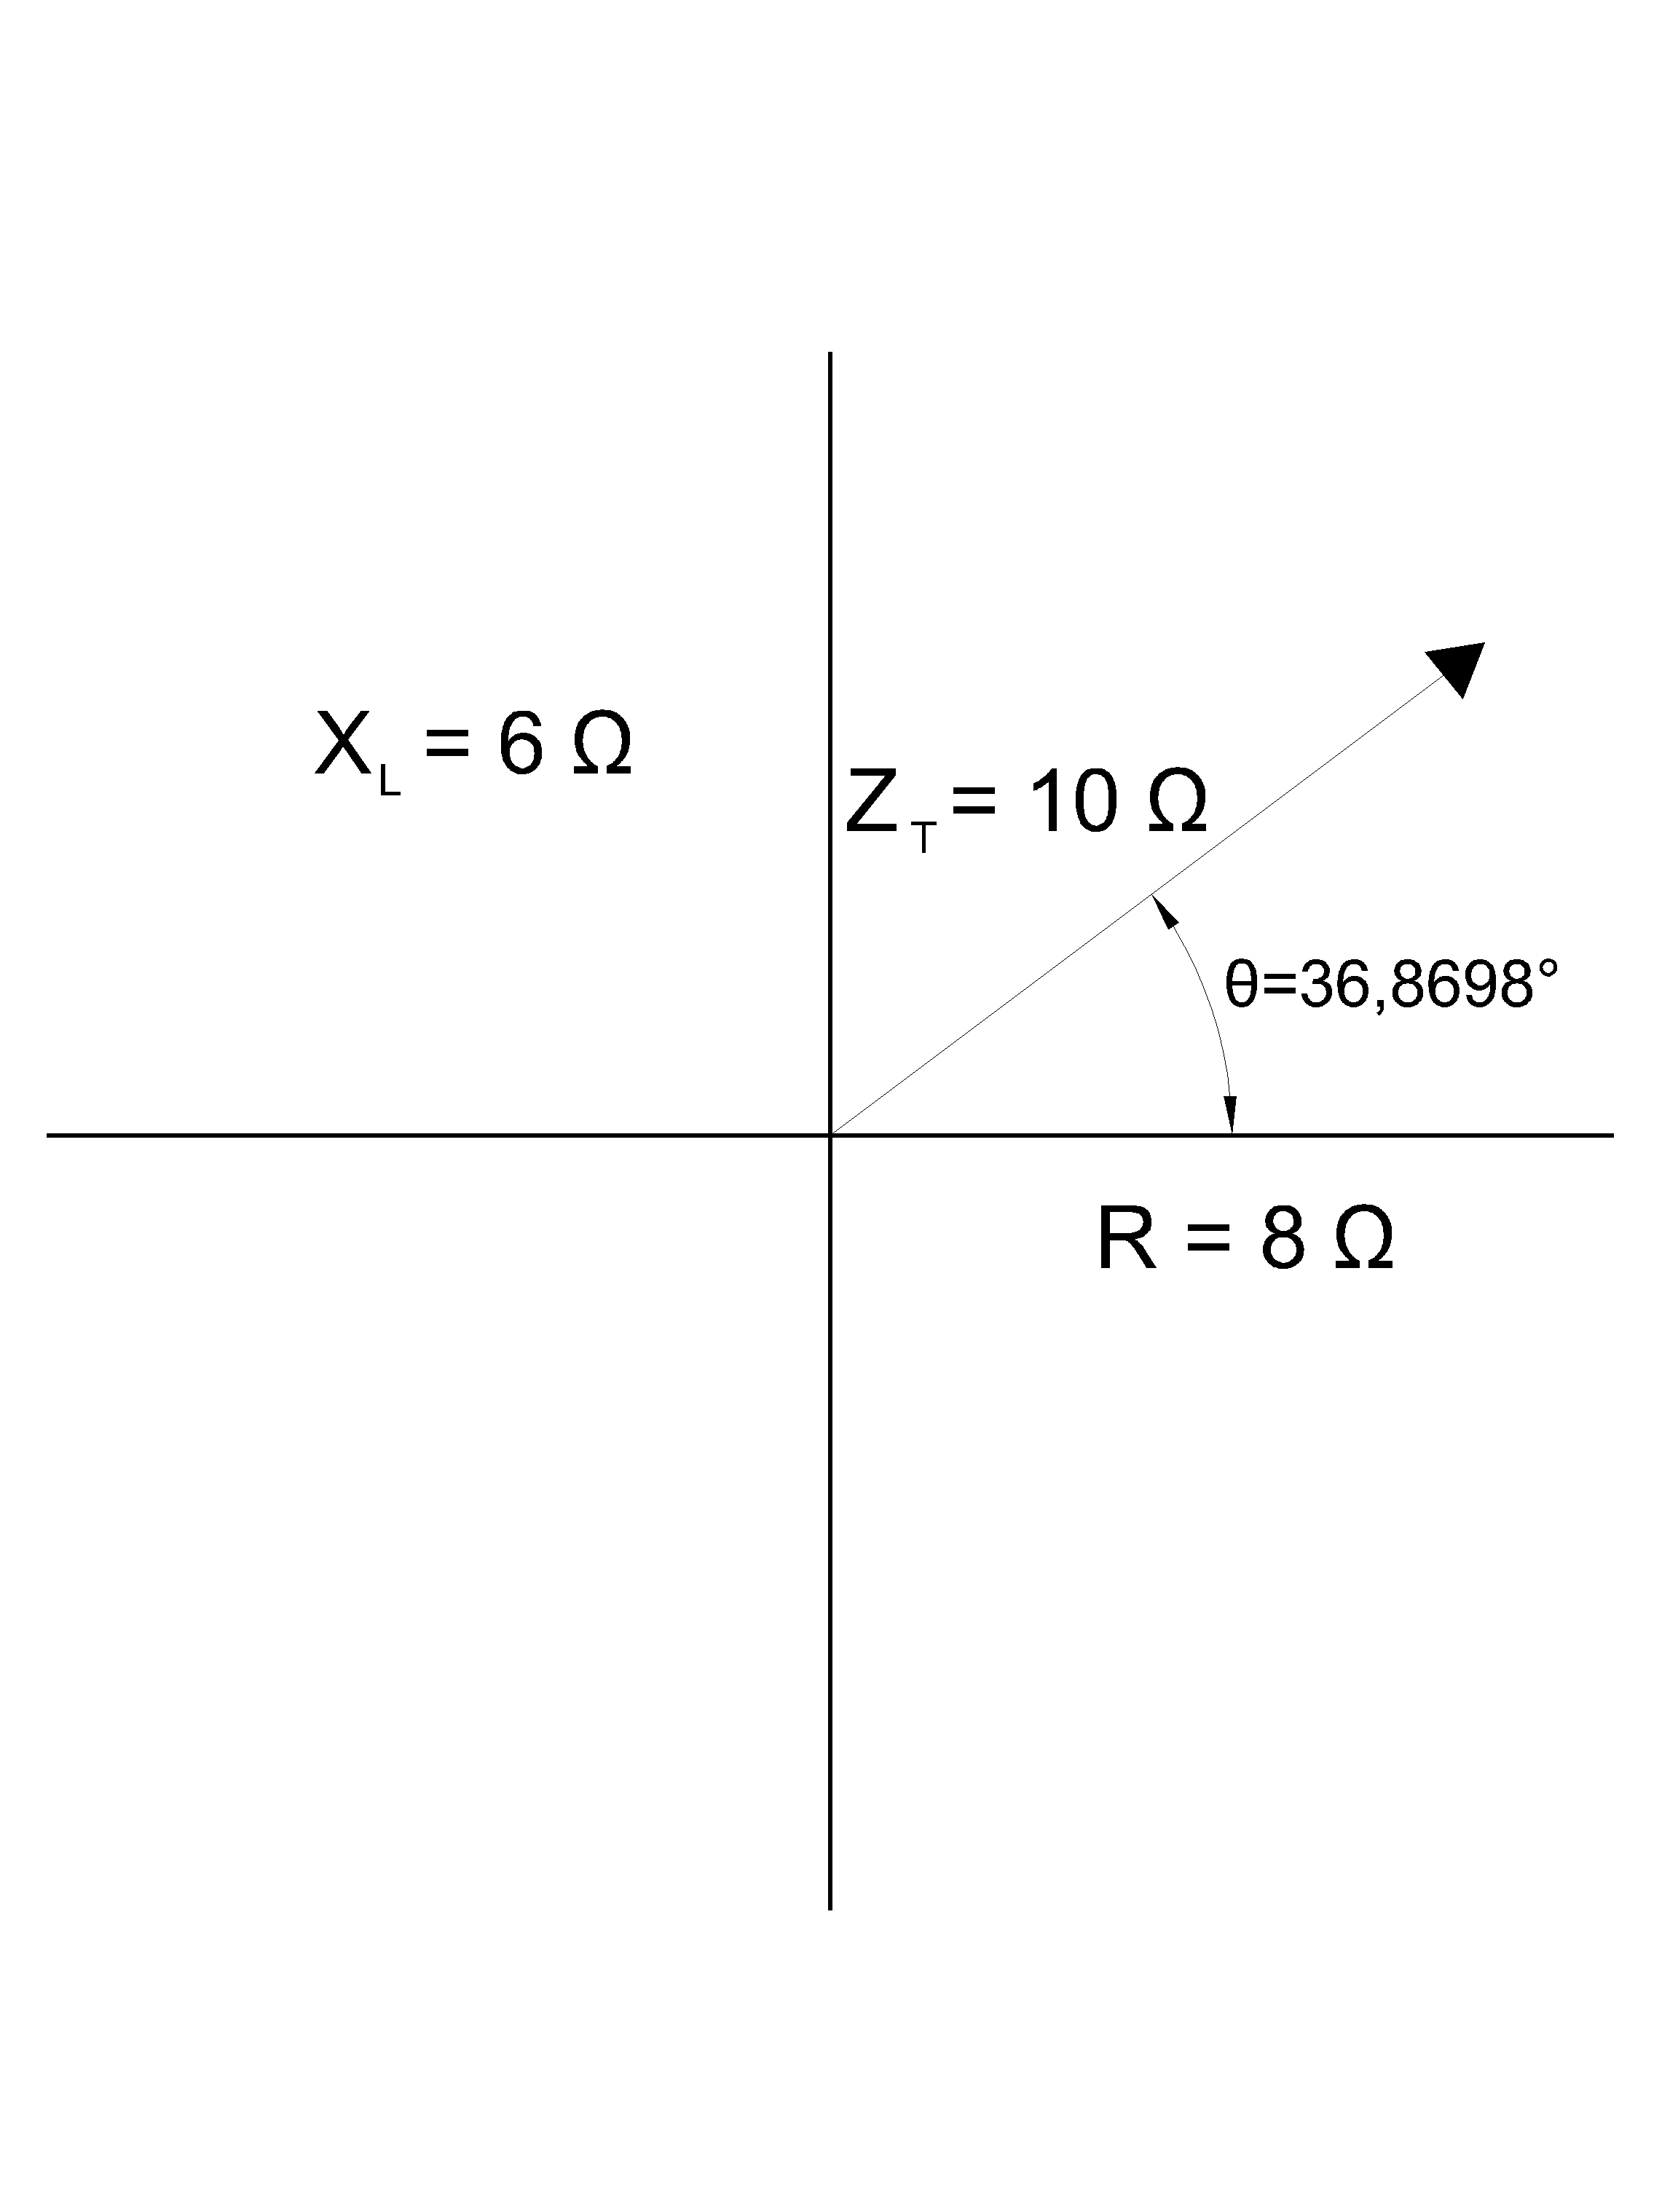
\includegraphics[scale= 0.1]{fe16.png}
		      \caption{Impedancia total en el plano}
		      \label{f1}
	      \end{figure}

	      Encontrar la corriente y los voltajes $V_R$ y $V_L$

	      \begin{align*}
		       & I=\frac{E}{Z_T}                               \\
		       & I=\frac{100<0}{10<36.8698}= 10<-36.8698       \\\\\
		       & V_R=IZ_R=(I<\theta)(R<0)=(10<-36.8698)(8<0)   \\
		       & V_R=80<-36.8698                               \\\\
		       & V_L=IZ_L=(I<\theta)(L<90)=(10<-36.8698)(6<90) \\
		       & V_L=60<53.13
	      \end{align*}

	      \begin{figure}[h!]
		      \centering
		      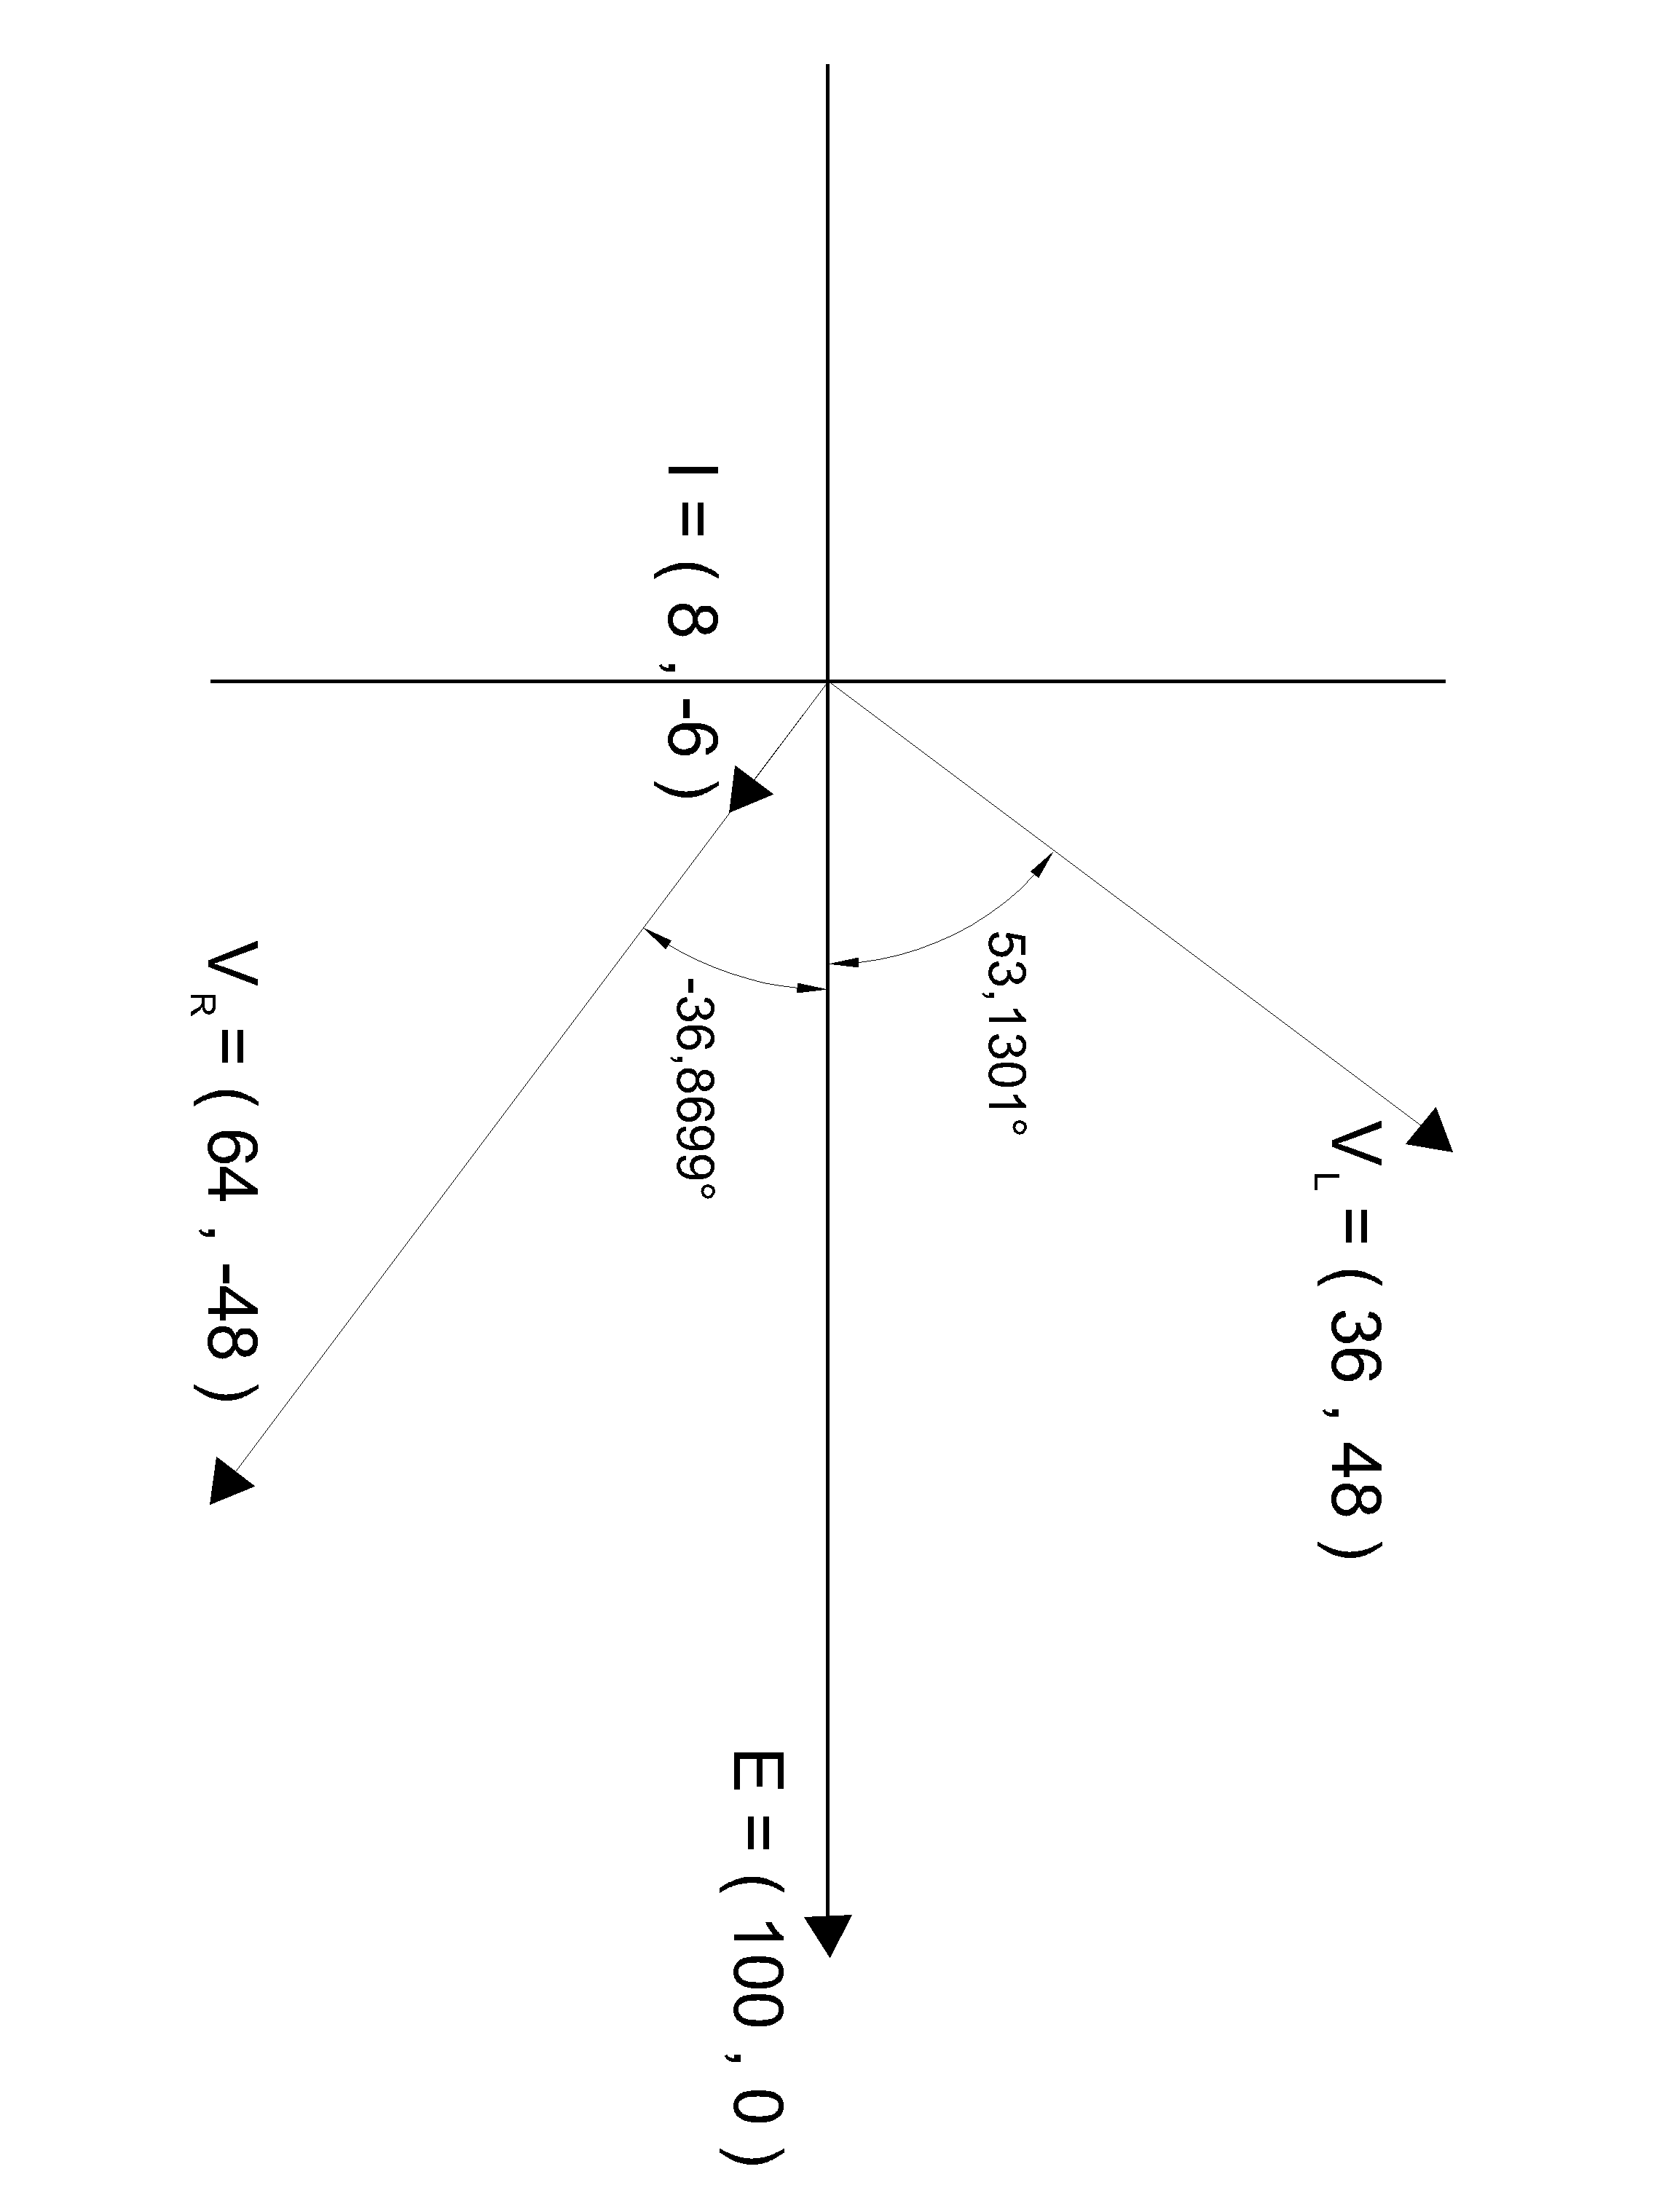
\includegraphics[scale= 0.1]{fe17.png}
		      \caption{Voltajes y corriente en el plano}
		      \label{f2}
	      \end{figure}

	      Verificar la ley de voltaje de Kirchhoff $V_T=V_R+V_C+V_L$

	      \begin{align*}
		       & V_R=80<-36.8698=64-j48  \\
		       & V_L=60<53.13=36+j48     \\\\\
		       & 100<0=(64-j48)+(36+j48) \\
		       & 100<0=100+J0            \\
		       & 100<0=100<0
	      \end{align*}

	      Encontrar la potencia promedio entregada al circuito.

	      \begin{align*}
		       & P=E I\cos{\theta_T}              \\
		       & P=(100<0)(10)(\cos{-36.8698})    \\
		       & P= 250 w                         \\\\
		       & F_P=\cos{\theta_T}= 0.8 Atrasado
	      \end{align*}

	      Encontrar la corriente y los voltajes en forma senoidal con una frecuencia de 60Hz
	      \begin{align*}
		       & V_R=80<-36.8698 & \implies 80\sqrt{2}\sen(2\pi60t-36.8698) \\
		       &                 & \implies113.1371sen(377t-36.8698)        \\\\\
		       & V_L=60<53.13    & \implies 60\sqrt{2}\sen(2\pi60t+53.13)   \\
		       &                 & \implies84.8528sen(377t+53.13)           \\\\\
		       & I=10<-36.8698   & \implies 10\sqrt{2}\sen(2\pi60t-36.8698) \\
		       &                 & \implies14.1421sen(377t-36.8698)         \\\\\
	      \end{align*}
	      %%%%%%%%%%%%%%%%%%%%%%%%%%%%%%%%%%%%%% PROBLEMA 6

	\item Para el circuito de la figura:


	      \begin{enumerate}
		      \item a. Encuentre la impedancia total $Z_T$ en forma polar.
		      \item Trace el diagrama de impedancia.
		      \item Encuentre el valor de C en microfarads y de L en henrys.
		      \item Encuentre la corriente $I$ y los voltajes $V_R$, $V_L$ y $V_C$ en forma fasorial.
		      \item Trace el diagrama fasorial de los voltajes E, $V_R$, $V_L$ y $V_C$, y de la corriente I.
		      \item Verifique la ley de voltaje de Kirchhoff alrededor del lazo cerrado.
		      \item Encuentre la potencia promedio entregada al circuito.
	      \end{enumerate}

	      \begin{center}
		      \begin{circuitikz}[american]
			      \draw (0,0) to [sV=$e{=}70.7\sin(\omega 337t)$](0,3) to [R=$R{=}2\Omega$, v=$v_R$] (2,3) ;
			      \draw (2,3) to [cute inductor= $X_L{=}6\Omega$,v=$v_L$](4,3);
			      \draw (4,3) to [cute inductor=$X_L{=}4\Omega$, v=$v_L$](6,3) to [I=$i$](6,0);
			      \draw  (0,0) to [I=$Z_T$](3,0) to (6,0);
		      \end{circuitikz}
	      \end{center}


	      \textit{ Sol. }


	      Convertir la fuente de voltaje del dominio del tiempo al dominio del fasor.

	      \begin{align*}
		      e=70.71\sen 377t & \implies E=50<0^{\circ}
	      \end{align*}


	      Ordenar las impedancias de la forma polar a la rectangular.
	      \begin{align*}
		       & Z_1=2<0=2+J0     \\
		       & Z_2=6<90=0+J6    \\
		       & Z_3=10<-90=0-J10 \\
	      \end{align*}


	      Encontrar $Z_t$ sumando todas las impedancias.
	      \begin{align*}
		       & Z_T=(2+j0)+(0+j6)+(0-j10) \\
		       & Z_T=2-j4
	      \end{align*}

	      Convertir $Z_T$ a su forma polar.
	      \begin{align*}
		       & Z_T=2-j4= 2\sqrt{5}<-63.4349
	      \end{align*}

	      Convertir C en mF y L en H.

	      \begin{align*}
		       & X_L=wL                              &  & L=\frac{X_L}{w}      \\
		       & L=\frac{6}{377rads/s}=0.016H                                  \\\\\\
		       & X_L=\frac{1}{wC}                    &  & C=\frac{1}{(w)(X_C)} \\
		       & C=\frac{1}{(377rads/s)(10)}=26.52mF
	      \end{align*}

	      \begin{figure}[h!]
		      \centering
		      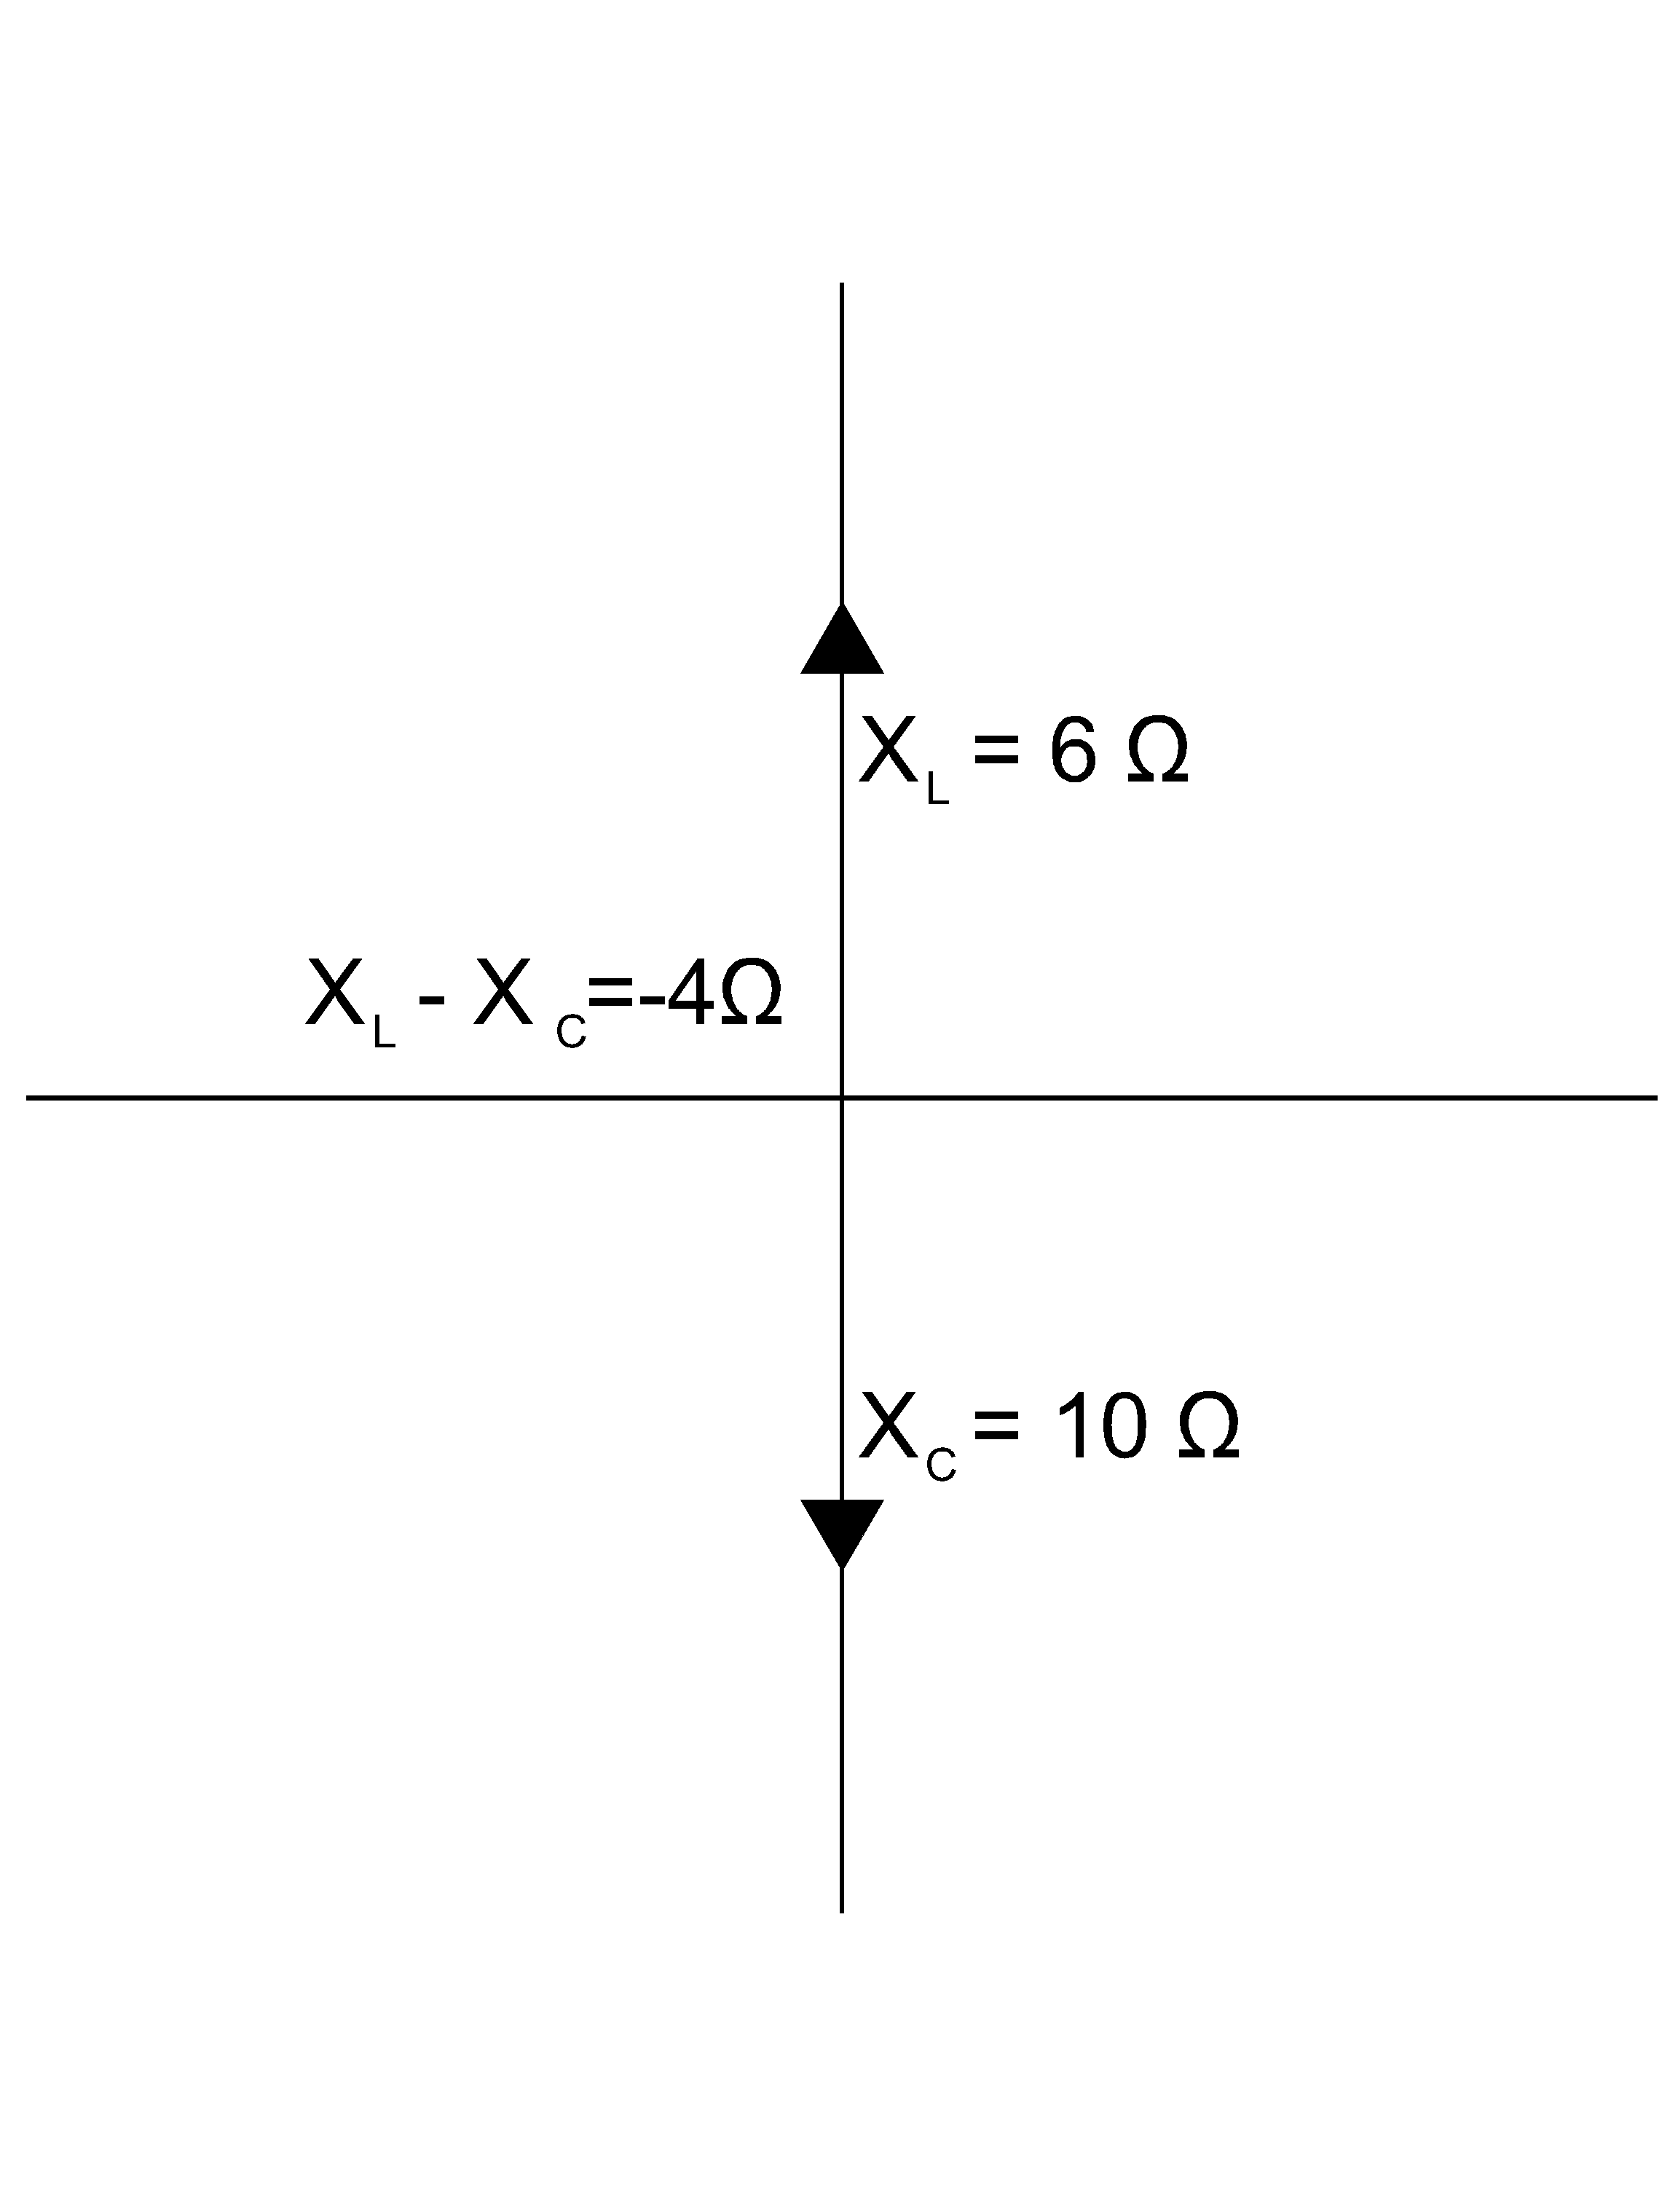
\includegraphics[scale= 0.1]{fe18.png}
		      \caption{Reactancias en el plano}
		      \label{f3}
	      \end{figure}

	      Encontrar la corriente y los voltajes $V_R, V_C, V_L$

	      \begin{align*}
		       & I=\frac{E}{Z_T}                                        \\
		       & I=\frac{50<0}{2\sqrt{5}<-63.4349}= 5\sqrt{5}<63.4349   \\\\\
		       & V_R=IZ_R=(I<\theta)(R<0)=(5\sqrt{5}<63.4349)(2<0)      \\
		       & V_R=10\sqrt{5}<63.4349                                 \\\\
		       & V_C=IZ_C=(I<\theta)(C<-90)=(5\sqrt{5}<63.4349)(10<-90) \\
		       & V_C=50\sqrt{5}<-26.5651                                \\\\
		       & V_L=IZ_L=(I<\theta)(L<90)=(5\sqrt{5}<63.4349)(6<90)    \\
		       & V_L=30\sqrt{5}<153.4349
	      \end{align*}

	      \begin{figure}[h!]
		      \centering
		      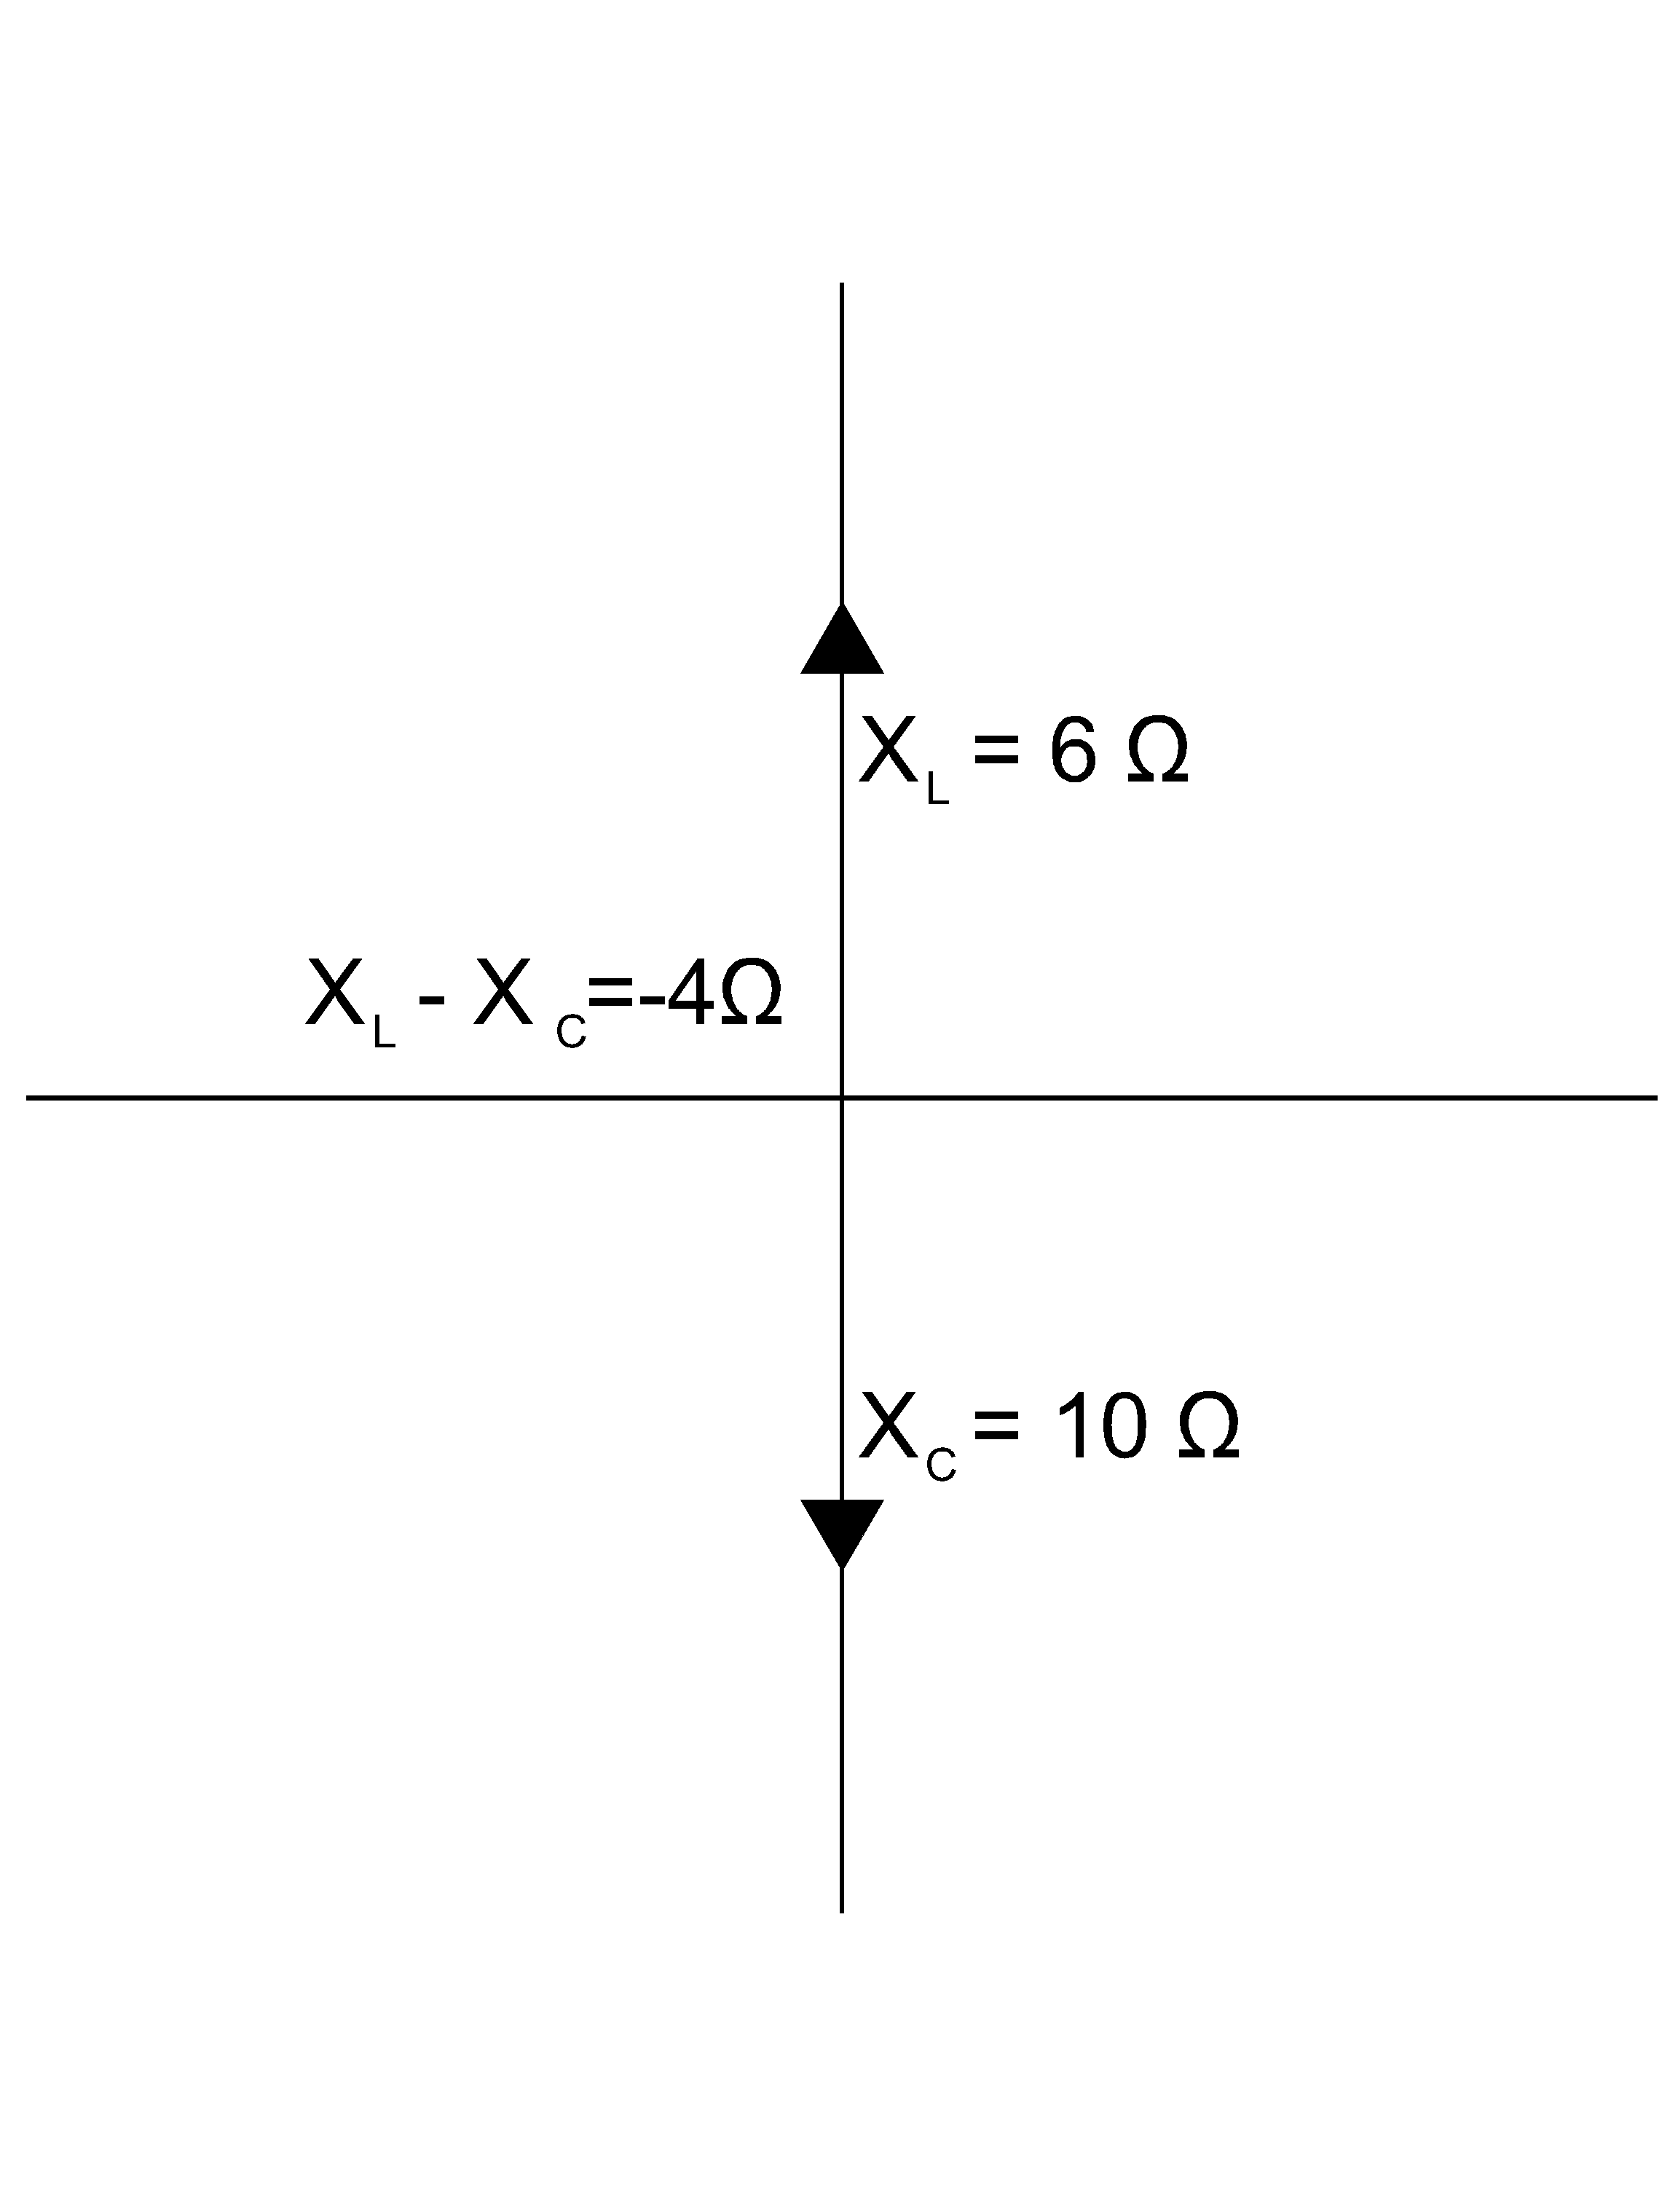
\includegraphics[scale= 0.1]{fe18.png}
		      \caption{Voltajes en el plano}
		      \label{f4}
	      \end{figure}

	      Verificar la ley de voltaje de Kirchhoff $V_T=V_R+V_C+V_L$

	      \begin{align*}
		       & V_R=10\sqrt{5}<63.4349=10+J20     \\
		       & V_C=50\sqrt{5}<-26.5651=100-J50   \\
		       & V_L=30\sqrt{5}<153.4349=-60+J30   \\\\\
		       & 50<0=(10+J20)+(100-J50)+(-60+J30) \\
		       & 50<0=50+J0                        \\
		       & 50<0=50<0
	      \end{align*}

	      Encontrar la potencia promedio entregada al circuito.

	      \begin{align*}
		       & P=E I\cos{\theta_T}                \\
		       & P=(50<0)(5\sqrt{5})(\cos{63.4349}) \\
		       & P= 250 w                           \\\\
		       & F_P=\cos{\theta_T}= 0.45 Atrasado
	      \end{align*}

	      %%%%%%%%%%%%%%%%%%%%%%%%%%%%%%%%%%%%%% PROBLEMA 7

	\item Utilice la regla del divisor de voltaje y calcule los voltajes $V_1$ y $V_2$ para el circuito de la figura en forma fasorial.


	      \begin{center}
		      \begin{circuitikz}[american]
			      \draw (0,0) to [sV=$E{=}60V<5^{\circ}$](0,3) to [R=$6.8\Omega$] (2,3);
			      \draw (2,3) to [cute inductor= $40\Omega$,v=$v_1$](4,3);
			      \draw (4,3) to [R=$9\Omega$,v=$v_2$](6,3) to (6,0);
			      \draw  (0,0) to [I=$Z_T$](3,0) to (6,0);
		      \end{circuitikz}
	      \end{center}


	      \textit{ Sol. }

	      Ordenar cada impedancia de manera polar a rectangular.

	      \begin{align*}
		       & Z_{R1}=6.8<0=6.8+j0 \\
		       & Z_L=40<90=0+j40     \\
		       & Z_{R2}=9<0=9+j0
	      \end{align*}


	      Y la impedancia total es:


	      \begin{equation}
		      Z_T=Z_{R1}+Z_L+Z_{R2}=6.8+j40+9=15.8+j40
	      \end{equation}

	      Y en forma polar:

	      \begin{equation}
		      Z_T=43.007<68.45
	      \end{equation}

	      Con estos datos procedemos a calcular $V_1$ con divisor de voltaje, usando la formula:

	      \begin{equation}
		      V_1=\frac{Z_LE}{Z_T}=\frac{(40<90)(60<5)}{43.007<68.45}=55.8<26.55
	      \end{equation}

	      Y para  el $V_2$ procedemos de igual forma:

	      \begin{equation}
		      V_2=\frac{Z_{R2E}}{Z_T}=\frac{(9<0)(60<5)}{43.007<68.45}=12.55<-63.45
	      \end{equation}

	      %%%%%%%%%%%%%%%%%%%%%%%%%%%%%%%%%%%%%% PROBLEMA 8

	\item Encuentre la admitancia total y la impedancia de los circuitos


	      \begin{align*}
		       & \begin{tikzpicture}[american]
			         \draw (-1,0) to [open, o-o] (-1,3) to [I=$Y_T$](1,3) to (3,3);
			         \draw (1,3) to [R=$22\Omega$](1,0) -- (-1,0);
			         \draw (3,3) to [curved capacitor=$6\Omega$](3,0) -- (1,0);
			         \draw(3,3) to (4.5,3) to [R=$22\Omega$] (4.5,0) to (3,0);
			         \draw (-1,0) to [I=$Z_T$](1,0);
		         \end{tikzpicture}
		       &                                                                & \begin{tikzpicture}[american]
			                                                                          \draw (-1,0) to [open, o-o] (-1,3) to [I=$Y_T$](1,3);
			                                                                          \draw (1,3) to [R=$3k\Omega$](1,0) -- (-0.9,0);
			                                                                          \draw (1,3) to (3,3) to [cute inductor=$6k\Omega$](3,0) -- (1,0);
			                                                                          \draw (3,3) to (4.5,3) to [curved capacitor=$9k\Omega$] (4.5,0) to (3,0);
			                                                                          \draw (-0.8,0) to [I=$Z_T$](1,0);
		                                                                          \end{tikzpicture}
	      \end{align*}


	      \textit{ Sol. }
	      Primer circuito:
	      Calculamos la resistencia equivalente, que es $11\Omega$
	      Procedemos a calcular las impedancias de la resistencia y del capacitor:

	      \begin{align*}
		       & Y_R=\frac{1}{11<0}=0.09<0=0.09+j0       \\
		       & Y_C=\frac{1}{6<-90}=0.16667<90=j0.16667
	      \end{align*}

	      Y la $Y_T$ la calculamos como sigue:
	      \begin{equation}
		      Y_T=Y_R+Y_C=0.09+j0.16667=0.189<61.63
	      \end{equation}
	      Y por ultimo calculamos la impedancia total
	      \begin{equation}
		      Z_T=\frac{1}{Y_T}=\frac{1}{0.189<61.63}=5.291<-61.63
	      \end{equation}


	      Ahora para el circuito 2 tenemos las siguientes impedancias:

	      \begin{align*}
		       & Z_3=3k\Omega <0   \\
		       & Z_L=6k\Omega <90  \\
		       & Z_C=9k\Omega <-90
	      \end{align*}

	      Por lo que sus correspondientes admitancias son:
	      \begin{align*}
		       & Y_R=\frac{1}{3k\Omega <0}=3.33\times10^{-4}<0=3.33\times 10^-4+j0        \\
		       & Y_L=\frac{1}{6k\Omega<90}=1.667\times10^{-4}<-90=0-j1.6667\times 10^{-4} \\
		       & Y_C=\frac{1}{9k\Omega <-90}=1.111\times10^{-4}<90=0+j1.11*10^{-4}        \\
	      \end{align*}


	      Procedemos a calcular la admitancia total sumando las admitancias obtenidas:
	      \begin{equation}
		      Y_T=3.33\times10^{-4}-j5.57\times10^{-5}=3.37\times10^{-4}<-9.5
	      \end{equation}
	      Y con la admitancia podemos calcular fácilmente la impedancia total:
	      \begin{equation}
		      Z_T=\frac{1}{Y_T}=\frac{1}{3.37\times10^{-4}<-9.5}=2967.36<9.5     \end{equation}




	      %%%%%%%%%%%%%%%%%%%%%%%%%%%%%%%%%%%%%% PROBLEMA 9

	\item Para el circuito de la figura:



	      \begin{center}
		      \begin{tikzpicture}[american]
			      \draw (0,3) to [sV, l_=$E{=}100V<0$](0,0);
			      \draw (2,3) to [R=$2\Omega$, i=$I_R$](2,0);
			      \draw (0,3) to [short, l_=$Y_T$, i=$I_s{=}2A<0$](2,3) to (4,3);
			      \draw (4,3) to[cute inductor=$X_L{=}5\Omega$, i=$I_L$] (4,0) to [ground](0,0);
		      \end{tikzpicture}
	      \end{center}

	      \begin{enumerate}
		      \item Encuentre la admitancia total $Y_T$ en forma polar.
		      \item Trace el diagrama de admitancia.
		      \item Encuentre el voltaje $E$ y las corrientes $I_R$ e $I_L$ en forma fasorial.
		      \item Trace el diagrama fasorial de las corrientes $I_s$, $I_R$ e IL, y del voltaje E.
		      \item Verifique la ley de corriente de Kirchhoff en un nodo.
		      \item Encuentre la potencia promedio entregada al circuito.
	      \end{enumerate}


	      \textit{ Sol. }
	      Primero vamos a pasar de forma triangular el valor de las impedancias de modo que quedarían de la siguiente manera:

	      \begin{align*}
		       & R=2\Omega = 2 \Omega <0^{\circ}   \\
		       & X_L=5 \Omega=5 \Omega <90^{\circ}
	      \end{align*}

	      Ahora como sabemos que están en paralelo quedarían:

	      \begin{equation*}
		      Z_T=\frac{(2<0)(5<90)}{(2<0)+(5<90)}= \frac{10<90}{5.38<68.19}=1.85<21.81
	      \end{equation*}

	      Al sacar la admitancia total:

	      \begin{equation*}
		      Y_T=\frac{1}{1.85<21.81}=0.54<-21.81
	      \end{equation*}

	      b) Diagrama

	      \begin{center}
		      \begin{circuitikz}[american]
			      \draw (1,1) to (-2,1) to [sV](-2,5) to (5,5);
			      \draw (1,1) to (5,1);
			      \draw (3,5) to [european resistor=$Y_1$](3,1);
			      \draw (5,5) to  [european resistor=$Y_2$](5,1);
		      \end{circuitikz}
	      \end{center}


	      c)Encontrar el voltaje E y las corrientes IR e IL en forma fasorial.

	      \begin{equation}
		      I_R=\frac{(I_s)(Z_L)}{Z_R+Z_L}=\frac{(2<0)(5<90)}{5.38<68.19}=\frac{10<90}{5.38<68.19}= 1.85A<21.81
	      \end{equation}
	      \begin{equation}
		      I_L=\frac{(2<0)(2<0)}{5.38<68.19}=\frac{4<0}{5.38<68.19}= 0.74A<-68.19
	      \end{equation}
	      Ahora solo tenemos que sacar el voltaje utilizando la formula V=IZ y se veria de la siguiente manera:
	      \begin{equation}
		      V=IZ=(2A<0^{\circ})(1.85<21.81)=3.7<21.81
	      \end{equation}
	      d) Diagrama fasorial

	      \begin{center}
		      \begin{circuitikz}[american]
			      \draw (1,1) to (-2,1) to [sV=$4V<0^{\circ}$](-2,5) to (5,5);
			      \draw (1,1) to (5,1);
			      \draw (3,5) to [european resistor=$Z_1$](3,1);
			      \draw (5,5) to  [european resistor=$Z_2$](5,1);
		      \end{circuitikz}
	      \end{center}


	      e)Verificar con la ley de la corriente de Kirchhoff
	      \begin{equation}
		      I_s=I_R+I_L
	      \end{equation}
	      \begin{equation}
		      (1.71+j0.68)+(0.27-j0.68)=1.98+j0
	      \end{equation}
	      \begin{equation}
		      2+j0= 2<0=I_S
	      \end{equation}
	      f)Encontrar la potencia promedio entregada al circuito.Esto lo haremos utilizando la siguiente fórumla:
	      \begin{equation}
		      P_T=ECos\theta_T
	      \end{equation}
	      Siguiendo la formula anterior sabemos que T representa la impedancia total, la cual será calculada de la siguiente manera:
	      \begin{equation}
		      P=(3.7)(2)Cos(21.81)=7.4cos(21.81)=6.87W
	      \end{equation}

	      %%%%%%%%%%%%%%%%%%%%%%%%%%%%%%%%%%%%%% PROBLEMA 10

	\item Para el circuito de la figura


	      \begin{center}
		      \begin{circuitikz}[american]
			      \draw (0,0) to [sV=$i_s{=}3\sin(\omega 337t+60)$](0,3) to  (2,3) ;
			      \draw (2,3) to [cute inductor= $X_L{=}6\Omega$,v=$v_L$](4,3);
			      \draw (4,3) to [cute inductor=$X_L{=}4\Omega$, v=$v_L$](4,0);
			      \draw (2,3) to [R=$R{=}2\Omega$, v=$v_R$](2,0);
			      \draw (4,3) to (7,3) to [cute inductor= $X_L{=}6\Omega$,v=$v_L$](7,0);
			      \draw (0,0) to (3,0) to (7,0);
		      \end{circuitikz}
	      \end{center}


	      \begin{enumerate}
		      \item Encuentre la admitancia total $Y_T$ en forma polar.
		      \item Trace el diagrama de admitancia.
		      \item Encuentre el valor de $C$ en microfarads y el de $L$ en henrys.
		      \item Encuentre el voltaje $E$ y las corrientes IR, $I_L$ e $I_C$  en forma fasorial.
		      \item Trace el diagrama fasorial de las corrientes $I_s$, IR, $I_L$ e $I_C$, y del voltaje $E$.
		      \item Verifique la ley de corriente de Kirchhoff en un nodo.
		      \item Encuentre la potencia promedio entregada al circuito.
		      \item Encuentre las expresiones senoidales para las corrientes y el voltaje.
	      \end{enumerate}



	      \textit{ Sol. }
	      a) Se suman las admitancias en paralelo de la siguiente manera:
	      \begin{equation}
		      \frac{1}{1.2<0}+\frac{1}{2<-90}+\frac{1}{5<90}= \frac{5}{6}+j3
	      \end{equation}
	      \begin{equation}
		      Y_T=\frac{\sqrt{706}}{30}<19.79
	      \end{equation}

	      b) Diagrama

	      \begin{center}
		      \begin{circuitikz}[american]
			      \draw (0,1) to (-2,1) to [sV](-2,5) to (5,5);
			      \draw (0,1) to (5,1);
			      \draw (1,5) to [european resistor=$Y_1$](1,1);
			      \draw (3,5) to [european resistor=$Y_2$](3,1);
			      \draw (5,5) to  [european resistor=$Y_3$](5,1);
		      \end{circuitikz}
	      \end{center}

	      c)Se hace el despeje de la formula $X_C=\frac{1}{WC}$ posteriormente se sustituyen valores para obtener del valor de C.
	      \begin{equation}
		      X_L=2\Omega=377L
	      \end{equation}
	      \begin{equation}
		      L=\frac{2}{377}=5.3050\times 10^{-3}
	      \end{equation}
	      \begin{equation}
		      5=\frac{1}{WC}
	      \end{equation}
	      \begin{equation}
		      C=\frac{1}{885}F=5.305mF
	      \end{equation}

	      d) Al calcular el valor de E y las corrientes de $I_R$, $I_L$ e $I_C$

	      \begin{equation}
		      E=\frac{I_T}{Z_T}=\frac{2.59<60}{1.129<-19.79}=2.29<79.79
	      \end{equation}
	      \begin{equation}
		      I_R=EY_R=(2.29<79.79)(\frac{1}{1.2}<0=1.90<79.79
	      \end{equation}
	      \begin{equation}
		      I_L=(2.29<79.79)(\frac{1}{2}<-90)=1.154<-10.21
	      \end{equation}
	      \begin{equation}
		      I_C=(2.29<79.79)(\frac{1}{5}<90)=0.458<169,7
	      \end{equation}

	      e)Diagrama Fasorial

	      f)Ley de Kirchhoff

	      g)Al calcular la potencia promedio:
	      \begin{equation}
		      P=EICos\theta
	      \end{equation}
	      \begin{equation}
		      P=5.93Cos(79.79)=1.0511W
	      \end{equation}
	      %%%%%%%%%%%%%%%%%%%%%%%%%%%%%%%%%%%%%% PROBLEMA 11

	\item Calcule las corrientes $I_1$ e $I_2$ de la figura en forma fasorial utilizando la regla del divisor de corriente.


	      \begin{center}
		      \begin{circuitikz}
			      \draw (2,0) to (0,0) to (0,3) to [short, i=$I{=}20A<40$](2,3) to [R=$33\Omega$](2,0) to (4,0) to [cute inductor=$XL_2{=}10\Omega$](4,1.5) to [cute inductor=$XL_1{=}60\Omega$](4,3) to (3,3) to (2,3);

			      \draw (6,0) to (6,1.5) to [short, i=$I_1$](6,3) to [cute inductor=$XL{=}4\Omega$, i=$I_1$](9,3) to (9,0) to [curved capacitor=$X_C{=}6\Omega$](8.50,0) to [R=$R{=}3\Omega$](6,0);
			      \draw (5,1.5) to [short, i=$I{=}6A<30$](6,1.5);
			      \draw (6,1.5) to [short, i=$I_1$](6,0);
		      \end{circuitikz}
	      \end{center}
	      \textit{ Sol. }
	      Para el primer diagrama comenzamos sumando las impedancias.
	      Posteriormente se empiezan a hacer los calculos para obtener el valor de las corrientes.
	      (Este procedimiento es para ambos diagramas)
	      \begin{equation}
		      \frac{1}{Z_T}=\frac{1}{33<0}+\frac{1}{70<-90}
	      \end{equation}
	      \begin{equation}
		      Z_T=\frac{2000}{67}<25.24
	      \end{equation}
	      \begin{equation}
		      I_1=(20A<40)(\frac{70<90}{\frac{200}{67}<25.24}
	      \end{equation}
	      \begin{equation}
		      I_1=46.9<104.79
	      \end{equation}
	      \begin{equation}
		      I_2=(20A<40)(\frac{33<0}{\frac{200}{67}<25.24}
	      \end{equation}
	      \begin{equation}
		      I_2=22.11<14.76
	      \end{equation}
	      Para el segundo diagrama
	      \begin{equation}
		      R_{IC}=3+j(-6)= 3\sqrt{5}<-63.43
	      \end{equation}
	      \begin{equation}
		      \frac{1}{R_IC}=3+j(-6+4)
	      \end{equation}
	      \begin{equation}
		      \frac{1}{R_IC}=\sqrt{13}<(33.69)
	      \end{equation}
	      \begin{equation}
		      I_1=\frac{(3\sqrt{5}<-63.45}{(\sqrt{13}<33.69}
	      \end{equation}
	      \begin{equation}
		      I_1=(1.860<-97.14)(6<30)
	      \end{equation}
	      \begin{equation}
		      I_1=11.16<-67.14
	      \end{equation}
	      \begin{equation}
		      I_2=(\frac{4<90}{\sqrt{13}<33.69})(6<30)
	      \end{equation}
	      \begin{equation}
		      I_2=6.654<86.31
	      \end{equation}
	      %%%%%%%%%%%%%%%%%%%%%%%%%%%%%%%%%%%%%% PROBLEMA 12

	\item Para la red en serie-paralelo de la figura

	      \begin{center}
		      \begin{circuitikz}[american]
			      \draw (0,0) to [sV=$E{=}12V<0$](0,3) to [cute inductor=$X_L{=}6\Omega$, v=$v_L$] (2,3) ;
			      \draw (2,3) to (4,3);
			      \draw (4,3) to (4,2) to [curved capacitor, l_=$X_C2{=}12\Omega$](6,2) to (6,3);
			      \draw (4,3) to [curved capacitor=$X_C{=}8\Omega$](6,3) to (7,3) to (7,0) to (0,0);
		      \end{circuitikz}
	      \end{center}

	      \begin{enumerate}
		      \item Calcule $Z_T$.
		      \item Determine $I$.
		      \item Determine $I_1$.
		      \item Encuentre $I_2$ e $I_3$.
		      \item Encuentre $VL$.
	      \end{enumerate}




	      \textit{ Sol. }

	      1.

	      Para resolver el problema y los incisos transformamos a la forma fasorial el circuito:

	      \begin{align*}
		       & Z_L=6 < 90^o= 0 + j6                           \\
		       & Z_C=20<-90^o=0 - j20                           \\
		       & Z_T=0 - j14                                    \\
		       & Z_T= \sqrt{0^2 + 14^2}< tan^{-1} \frac{-14}{0} \\
		       & Z_T=14<0^o
	      \end{align*}

	      2.
	      \begin{align*}
		       & V=Z \cdot I                                                     \\
		       & I= \frac{V}{Z} = \frac{12<0^o}{14<0^o}= \frac{12}{14}<0^o - 0^o \\
		       & I=\frac{6}{7}<0^o
	      \end{align*}

	      3.
	      \begin{align*}
		       & I_1=\frac{V}{Z}=\frac{12<0^O}{6<90^o} \\
		       & I_1=2<-90^o
	      \end{align*}

	      4.
	      \begin{align*}
		       & I_2=\frac{12<0^O}{8<-90^o}  \\
		       & I_2=\frac{3}{2}<90^o        \\
		       & I_3=\frac{12<0^O}{12<-90^o} \\
		       & I_3=1<90^o
	      \end{align*}

	      5.
	      \begin{align*}
		       & V_L=Z \cdot I              \\
		       & V_L=(6<90^o)\cdot(2<-90^o) \\
		       & V_L=12<0^o
	      \end{align*}

	      %%%%%%%%%%%%%%%%%%%%%%%%%%%%%%%%%%%%%% PROBLEMA 13

	\item Para la red de la figura:


	      \begin{center}
		      \begin{circuitikz}[american]
			      \draw (0,0) to [sV=$E{=}30V<0$](0,3) to [R=$R_1{=}3\Omega$](2,3) ;
			      \draw (2,3) to [cute inductor=$X_L{=}6\Omega$, v=$v_L$](4,3);
			      \draw (4,4) to (4,2) to [curved capacitor, l_=$X_{C2} {=}12\Omega$](6,2) to (6,4);
			      \draw (4,4) to [R=$R_2{=}2\Omega$](6,4);
			      \draw (6,3) to [I=$I_C$](7,3) to (7,0) to (0,0);
			      \draw (0,1.5) to [short, i=$Z_T$](0,0);
			      \draw (0,1.5) to [short, i=$I_S$](0,3);
		      \end{circuitikz}
	      \end{center}

	      \begin{enumerate}
		      \item Encuentre la impedancia total $Z_T$.
		      \item Determine la corriente $I_s$.
		      \item Calcule $IC$ utilizando la regla del divisor de corriente.
		      \item Calcule $V_L$ utilizando la regla del divisor de voltaje.
	      \end{enumerate}


	      \textit{ Sol. }

	      Para resolver todos los incisos del problema, simplificamos a su forma factorial el circuito, teniendo:\\
	      \begin{align*}
		       & Z_1=Z_R = 3 < 0^o                                        \\
		       & Z_2=Z_L = 6 < 90^o                                       \\
		       & Z_3=Z_R + Z_C = \frac{16<-90^o}{(2+j0)(0-j8)}            \\
		       & Z_3=\frac{16<-90^o}{2-j8}=\frac{16<-90^o}{8.25<-75.96^o} \\
		       & Z_3=1.94<-14.04^O = 1.88 - j 0.47
	      \end{align*}

	      1.
	      \begin{align*}
		       & Z_T=(3+j0)(0+j6)(1.88+j0.47)=4.88+j5.53 \\
		       & Z_T=7.38 < 48.57^o
	      \end{align*}

	      2.
	      \begin{align*}
		       & I_s=\frac{30V<0^o}{7.38<48.57^o} \\
		       & I_s=4.07<-48.57^o
	      \end{align*}

	      3.
	      \begin{align*}
		       & I_c=\frac{Z_R \cdot Z_c + Z_R} = \frac{(2<0^o)(4.07<-48.57^o)}{8.25<-75.96^o} \\
		       & I_c=\frac{8.14<-48.57^o}{8.25<-75.46^o}=0.99<26.89^o                          \\
		       & I_c= 1 < 26.9^o
	      \end{align*}

	      4.
	      \begin{align*}
		       & V_L=\frac{Z_L \cdot E}{Z_T}=\frac{(6<90^O)(30V<0^o)}{7.38<48.57^o} \\
		       & V_L=\frac{180<90^o}{7.38<48.57}                                    \\
		       & V_L=24.4< 47.43^o
	      \end{align*}

	      %%%%%%%%%%%%%%%%%%%%%%%%%%%%%%%%%%%%%% PROBLEMA 14

	\item Para la red de la figura


	      \begin{center}
		      \begin{circuitikz}[american]
			      \draw (-1,0) to [sV=$E{=}30V<0$](-1,3) to [R=$R_1{=}3\Omega$](1,3);
			      \draw (3,3) to (4,3);
			      \draw (4,4) to (4,2) to [cute inductor=$X_{L2}{=}3\Omega$, v=$v_L$](6,2) to (6,4);
			      \draw (4,4) to [R=$R_2{=}2\Omega$](6,4);
			      \draw (6,3) to [I=$I_C$](7,3) to (7,0) to (-1,0);
			      \draw (-1,1.5) to [short, i=$Z_T$](-1,0);
			      \draw (-1,1.5) to [short, i=$I_S$](-1,3);
			      \draw (4,3) to [R=$R_3{=}8\Omega$](6,3);
			      \draw (1,2) to (1,4) to [curved capacitor, l_=$X_{C2}{=}12\Omega$](3,4) to (3,2) to [cute inductor=$X_L{=}6\Omega$](1,2);
		      \end{circuitikz}
	      \end{center}

	      \begin{enumerate}
		      \item Encuentre la impedancia total $Z_T$.
		      \item Calcule el voltaje $V_2$ y la corriente IL.
	      \end{enumerate}

	      \textit{ Sol. }

	      \begin{enumerate}
		      \item \begin{align*}
			             & Z_{R1}=2<0=2+j0                                                                 \\
			             & Z_C=46-90=0-j4                                                                  \\
			             & Z_{L1}=6<90=0+j6                                                                \\
			             & Z_{R2}=8<0=8+j0                                                                 \\
			             & Z_{R3}=8<0=8+j0                                                                 \\
			             & Z_{L2}=3<90=0+j3                                                                \\
			             & Z_{R2}\mid R_{ZR3}=\frac{(8<0)(8<0)}{(8<0)+(8<0)}=\frac{64<0}{16+j_0}=4<0=4+j_0
		            \end{align*}

		      \item \begin{align*}
			             & Z_{R23}+Z_{L2}=Z_1                                       \\
			             & Z_1=\frac{(4<0)(3z90)}{(4+j0)+(0+j3)}=\frac{12<90}{4+j3} \\
			             & Z_1=\frac{12<90}{5<36.8698}=2.4<53.13                    \\
			             & Z_1=1.44+j1.919
		            \end{align*}

		            Para la segunda impedancia, resolvemos:

		            \begin{align*}
			             & Z_2=Z_C\mid\mid Z_{L1}=\frac{(4<-09)(6<90)}{(0-j4)+(0+j6)}=\frac{24<0}{0+j2}=\frac{24<0}{2<90}=12<-90 \\
			             & Z_2=0-j12
		            \end{align*}

		            Y ya se tienen los elementos para calcular la impedancia total:

		            \begin{align*}
			             & Z_T=2R_1+Z_2+Z_1=(+j0)+(0-j12)+(1.44+j1.919)=3.44-j10.081                               \\
			             & Z_T=10.6517<-71.15                                                                      \\
			             & V_T=(5A<0)(10.6517<-17.15)=53.2585<-17.15                                               \\
			             & \text{Aplicando divisor de voltaje: }(53.26)\left(\frac{2.4<53.13}{3.44-j10.081}\right) \\
			             & =53.26\left(\frac{2.4<53.13}{10.6517<71.15}\right)=(53.26<-71.15)(0.2625<-1859)         \\
			             & V_2=11.98<-53.13
		            \end{align*}

		      \item Para encontrar $I_2$, se saben los siguientes datos:

		            \begin{align*}
			             & I_T=54<0 &  & Z_{A23}=4<0=4+j0 &  & Z_{L2}=3<90=0+j3
		            \end{align*}
		            Con el divisor de corriente, se resuelve:

		            \begin{align*}
			             & I_2=I_T\left(\frac{Z_{R23}}{Z_{R23}+Z_{L2}}\right)=5A<0\left(\frac{4<0}{(4+j0)+(0+j3)}\right) \\
			             & =5A<0\left(\frac{4<0}{4+j3}\right)=\frac{4<0}{5<36.86}=0.8<-36.36                             \\
			             & I_2=4A<-36.86
		            \end{align*}
	      \end{enumerate}

	      %%%%%%%%%%%%%%%%%%%%%%%%%%%%%%%%%%%%%% PROBLEMA 15

	\item Para la red de la figura


	      \begin{enumerate}
		      \item Encuentre la impedancia total $Z_T$ y la admitancia $Y_T$.
		      \item Encuentre las corrientes $I_1, I_2$ e $I_3$.
		      \item Verifique la ley de corriente de Kirchhoff demostrando que $Is = I_1 = I_2 = I_3$.
	      \end{enumerate}


	      \begin{center}
		      \begin{tikzpicture}[american]
			      \draw (-1,0) to[sV=$E{=}60V<0$] (-1,3) to [I=$I_S$](1,3) to [short, i=$I_1$](3,3);
			      \draw (2,3)to [cute inductor=$X_{L1}{=}1\Omega$](2,1.5) to [R=$R_1{=}20\Omega$](2,0);
			      \draw (3,3) to (5,3) to [R=$R_2{=}3\Omega$, i=$I_2$](5,0) -- (2,0);
			      \draw (5,3) to (7,3) to [R=$R_3{=}16V$](7,1.5) to [curved capacitor=$X_C{=}7\Omega$](7,0) to [cute inductor=$X_{L2}{=}15\Omega$](5,0) to (-1,0);
		      \end{tikzpicture}
	      \end{center}

	      \textit{ Sol. }

	      \begin{enumerate}
		      \item Para calcular la impediancia $Z_3$

		            \begin{align*}
			             & Z_{L1}=1<90^{\circ}=0+j1  &  & Z_1=Z_{L1}+Z_{R1}           \\
			             & Z_{R1}=2<0^{\circ}=2+j0   &  & Z_1=(0+j1)+(2+j0)=2+j1      \\
			             & Z_{R2}=2<0^{\circ}=3+j0   &  & Z_1=2.236<26.56=+2j1        \\
			             & Z_{C}=7<-90^{\circ}=0-j7  &  & Z_2=Z_{R2}=3<0^{\circ}=3+j0 \\
			             & Z_{L}=15<90^{\circ}=0+j15 &  & Z_3=Z_{R3}+2C+Z_{L2}        \\
		            \end{align*}

		            Se obtiene la siguiente equivalencia:

		            \begin{equation}
			            Z_3=Z_{R3}+Z_C+Z_{L2}=(16+j0)+(0-j7)+(0+j15)
		            \end{equation}

		            Por lo tanto $Z_3=(16+j8)=17.88<26.56$

		      \item Para sumar las impedancias, las transformamos a $Y$:

		            \begin{align*}
			             & Y_1=\frac{1}{2.3<26.56}=0.448<-26.56=0.436-j0.218    \\
			             & Y_2=\frac{1}{3<0}=0.33<0=0.33+j0                     \\
			             & Y_3=\frac{1}{17.88<26.56}=0.0559<-26.56=0.05-j0.0249
		            \end{align*}
		            Finalmente tenemos los resultados de:

		            \begin{align}
			             & Y_T=0.816-j0.2429=0.8516<16.57                       \\
			             & Z_T=\frac{1}{Y_T}=\frac{1}{0.8513<16.57}=1.17<-16.57
		            \end{align}

		      \item Teniendo ya la $Z_T$, se procede a calcular la resistencia total:

		            \begin{equation*}
			            I_T=\frac{60V<0^{\circ}}{1.17<-16.57}=15.28<16.57
		            \end{equation*}

		            Por lo tanto $I_5=49.15+j14.62$

		            Al estar en paralelo, la corriente en cada rama está determinada por $V_T$ y cada impedancia:

		            \begin{align*}
			             & I_1=\frac{60V<0}{2.23<26.56}=26.9<-26.56=24j12   \\
			             & I_2=\frac{60V<0}{3<0}=20<0=20+j0                 \\
			             & I_3=\frac{60<0}{17.88<26.456}=3.35<-26.56=3-j1.5
		            \end{align*}

		            \begin{equation}
			            I_1+I_2+I_3=47-j13.5\implies I_5=49.15+j13.63
		            \end{equation}
	      \end{enumerate}
\end{enumerate}